%%%%%%%%%%%%%%%%%%%%%%%%%%%%%%%%%%%%%%%%%%%%%%%%%%%
%
%  New template code for TAMU Theses and Dissertations starting Fall 2012.  
%  For more info about this template or the 
%  TAMU LaTeX User's Group, see http://www.howdy.me/.
%
%  Author: Wendy Lynn Turner 
%
%%%%%%%%%%%%%%%%%%%%%%%%%%%%%%%%%%%%%%%%%%%%%%%%%%%

\documentclass[12pt]{report}
\usepackage[letterpaper]{geometry}
\geometry{verbose,tmargin=1.25in,bmargin=1.25in,lmargin=1.4in,rmargin=1.15in}
 \usepackage[doublespacing]{setspace}
 \usepackage{tocloft}
 \usepackage[rm, tiny,center, compact]{titlesec}
 \usepackage{indentfirst}
 \usepackage{etoolbox}
\usepackage{tocvsec2}
 \usepackage[titletoc]{appendix}
 \usepackage{appendix}
 \usepackage{tamuconfig}
\usepackage{rotating}
%Graphics
\usepackage{float}
\usepackage{xcolor,graphicx}
%Math stuff
\usepackage{amsmath}
\usepackage{mathptmx}
\usepackage[mathscr]{euscript}
\newcommand{\vr}{\vec{r}}
\newcommand{\vo}{\vec{\Omega}}
%Changing spacing in itemized lists
\usepackage{enumitem}
\setlist{nosep}
%Include a pdf file
\usepackage{pdfpages}
%Algorithm
\usepackage{algorithm}
\usepackage{algorithmic}
\renewcommand{\arraystretch}{1}
\usepackage{caption}
\usepackage{array}
\newcolumntype{L}{>{\centering\arraybackslash}m{3cm}}
\newcommand{\tcr}[1]{\textcolor{red}{#1}}
%Creating a norm command
\newcommand{\norm}[1]{\left\lVert#1\right\rVert}
%Allow page breaks within align
\allowdisplaybreaks
\usepackage{listings}

\usepackage{etoolbox}% http://ctan.org/pkg/etoolbox
\makeatletter
% \patchcmd{<cmd>}{<search>}{<replace>}{<succes>}{<failure>}
\patchcmd{\@chapter}{\addtocontents{lof}{\protect\addvspace{10\p@}}}{}{}{}% LoF
\makeatother

% Added to fix issues with pdf searching in some versions of LaTeX
%\usepackage[T1]{fontenc}\usepackage{lmodern}
%%%%%%%%%%%%%%%%%%%%%%%%%%%%%

% Hyperref setup below.  You should be able to get away with using uncommenting just the first line.
%\usepackage[hidelinks]{hyperref}

% if \usepackage[hidelinks]{hyperref} doesn't work try this.
% \usepackage{hyperref}  % Hidelinks is an option that removes link visiability.  TAMU Thesis Offices prefers to not see the links. But often doesn't work.  
% 
% \hypersetup{
%     colorlinks=true,
%     linkcolor=black,
%     citecolor=black,
%     filecolor=black,
%     urlcolor=black,
% }
%%%%%%%  End of hyperref setup.  One of these two options should work, but my motto with hyperref is when in doubt, comment it out!
%%%%%%%%%  This hopefully fixes the problem with vertical spacing of section headings at the top of the page..  Commented out in 1.0.7
% \preto\section{%
% \ifnum\value{section}>0\addtocontents{toc}{\vskip-6pt}\fi
% }
% \preto\subsection{%
% \ifnum\value{subsection}=0\addtocontents{toc}{\vskip-6pt}\fi
% \ifnum\value{subsection}>0\addtocontents{toc}{\vskip-6pt}\fi
% } 
%%%%%%%%%%%%%%%%%%%%%%%%%%%%%%%%%%%%%%%%%%%%%%%%%%%%%%

\begin{document}

\renewcommand{\tamumanuscripttitle}{Load Balancing Unstructured Meshes for Massively Parallel Transport Sweeps}
\renewcommand{\tamupapertype}{Thesis}
\renewcommand{\tamufullname}{Tarek Habib Ghaddar}
\renewcommand{\tamudegree}{Master of Science}
\renewcommand{\tamuchairone}{Jean C. Ragusa}
% Uncomment out the next line if you have co-chairs.  You will also need to edit the titlepage.tex file.
%\newcommand{\tamuchairtwo}{Additional Chair Name}
\renewcommand{\tamumemberone}{Jim E. Morel}
\newcommand{\tamumembertwo}{Bojan Popov}
\renewcommand{\tamudepthead}{Yassin Hassan}
\renewcommand{\tamugradmonth}{May}
\renewcommand{\tamugradyear}{2016}
\renewcommand{\tamudepartment}{Nuclear Engineering}


%%%%%%%%%%%%%%%%%%%%%%%%%%%%%%%%%%%%%%%%%%%%%%%%%%%
%
%  New template code for TAMU Theses and Dissertations starting Fall 2012.  
%  For more info about this template or the 
%  TAMU LaTeX User's Group, see http://www.howdy.me/.
%
%  Author: Wendy Lynn Turner 
%	 Version 1.0 
%  Last updated 8/5/2012
%
%%%%%%%%%%%%%%%%%%%%%%%%%%%%%%%%%%%%%%%%%%%%%%%%%%%

%%%%%%%%%%%%%%%%%%%%%%%%%%%%%% 
%% TITLE PAGE
%% The values get updated automatically.  Please do not make changes to this file other than adding/deleting committee members where necessary.
%%%%%%%%%%%%%%%%%%%%%%%%%%%%%%

\providecommand{\tabularnewline}{\\}



\begin{titlepage}
\begin{center}
\MakeUppercase{\tamumanuscripttitle}
\vspace{4em}

A \tamupapertype

by

\MakeUppercase{\tamufullname}

\vspace{4em}

\begin{singlespace}

Submitted to the Office of Graduate and Professional Studies of \\
Texas A\&M University \\

in partial fulfillment of the requirements for the degree of \\
\end{singlespace}

\MakeUppercase{\tamudegree}
\par\end{center}
\vspace{2em}
\begin{singlespace}
\begin{tabular}{ll}
 & \tabularnewline
& \cr
% If you have Co-Chairs comment out the 'Chair of Committee' line below and uncomment the 'Co-Chairs of Committee' line.
Chair of Committee, & \tamuchairone\tabularnewline
%Co-Chairs of Committee, & \tamuchairone\tabularnewline & \tamuchairtwo\tabularnewline
Committee Members, & \tamumemberone\tabularnewline
 & \tamumembertwo\tabularnewline
Head of Department, & \tamudepthead\tabularnewline

\end{tabular}
\end{singlespace}
\vspace{3em}

\begin{center}
\tamugradmonth \hspace{2pt} \tamugradyear

\vspace{3em}

Major Subject: \tamudepartment \par
\vspace{3em}
Copyright \tamugradyear \hspace{.5em}\tamufullname 
\par\end{center}
\end{titlepage}
\pagebreak{}




 % This is simply a file that formats and adds your titlepage, please do not edit this unless you have a specific need. .
%%%%%%%%%%%%%%%%%%%%%%%%%%%%%%%%%%%%%%%%%%%%%%%%%%%
%
%  New template code for TAMU Theses and Dissertations starting Fall 2016.  
%
%
%  Author: Sean Zachary Roberson
%  Version 3.17.09
%  Last Updated: 9/21/2017
%
%%%%%%%%%%%%%%%%%%%%%%%%%%%%%%%%%%%%%%%%%%%%%%%%%%%
%%%%%%%%%%%%%%%%%%%%%%%%%%%%%%%%%%%%%%%%%%%%%%%%%%%%%%%%%%%%%%%%%%%%%
%%                           ABSTRACT 
%%%%%%%%%%%%%%%%%%%%%%%%%%%%%%%%%%%%%%%%%%%%%%%%%%%%%%%%%%%%%%%%%%%%%

\chapter*{ABSTRACT}
\addcontentsline{toc}{chapter}{ABSTRACT} % Needs to be set to part, so the TOC doesnt add 'CHAPTER ' prefix in the TOC.

\pagestyle{plain} % No headers, just page numbers
\pagenumbering{roman} % Roman numerals
\setcounter{page}{2}

\indent The field of radiation transport studies the distribution of radiation throughout a seven-dimensional phase-space consisting of time, space, energy, and direction. Radiation transport is described by the Boltzmann equation and can be solved stochastically or deterministically.

The work presented in this dissertation utilizes the deterministic method known as the transport sweep, a popular technique that has been the subject of a large amount of research.
We specifically focus on the parallel implementations of the transport sweep, and predicting the time it takes to sweep across a structured or unstructured mesh given a set of partitioning parameters, achieved through a time-to-solution estimator, written in Python.
The time-to-solution estimator is tested against PDT, Texas A\&M's massively deterministic transport code.
The time-to-solution estimator's sweep time is within 10\% of PDT's sweep time for the majority of problems tested.

We use the time-to-solution estimator as the objective function in an optimization scheme to attempt to get the partitions that lead to the fastest sweep time for a given problem and partitioning scheme.
Two optimization methods are discussed: using a black box tool (scipy's optimize library) and an intuitive method that relies on placing partitions in mesh locations that does not increase the number of cells (which we chose to name the CDF method).
The time-to-solution estimator proved to not be smooth enough for a black box tool to work, so the geometry based optimization method became the primary method.
The CDF method proved effective for our unbalanced pin test problem, improving the time to solution over previously used partitioning schemes.
For our larger test problem, the optimized partitioning scheme improves the time to solution over one previously used partitioning scheme, but is not as effective relative to other previously used partitioning schemes.
\pagebreak{}

%%%%%%%%%%%%%%%%%%%%%%%%%%%%%%%%%%%%%%%%%%%%%%%%%%%
%
%  New template code for TAMU Theses and Dissertations starting Fall 2016.  
%
%
%  Author: Sean Zachary Roberson
%  Version 3.17.09
%  Last Updated: 9/21/2017
%
%%%%%%%%%%%%%%%%%%%%%%%%%%%%%%%%%%%%%%%%%%%%%%%%%%%


%%%%%%%%%%%%%%%%%%%%%%%%%%%%%%%%%%%%%%%%%%%%%%%%%%%%%%%%%%%%%%%%%%%%%%
%%                           ACKNOWLEDGMENTS
%%%%%%%%%%%%%%%%%%%%%%%%%%%%%%%%%%%%%%%%%%%%%%%%%%%%%%%%%%%%%%%%%%%%%
\chapter*{ACKNOWLEDGMENTS}
\addcontentsline{toc}{chapter}{ACKNOWLEDGMENTS}  % Needs to be set to part, so the TOC doesnt add 'CHAPTER ' prefix in the TOC.


\indent I would like to thank Dr. Jean Ragusa for toeing the line between demanding and understanding perfectly. I know I haven't made your job as my advisor easy. 

Thank you to my committee, Drs. Adams, Amato, and Morel, for the feedback and advice when needed to push this work to completion.

A special thank you to Daryl Hawkins, a man I'm convinced is the most overworked code developer on the planet. This work would have been impossible without him. 

Thank you to Andrew Till for always being a sounding board for academic ideas, and thank you to Ian Halvic for dealing with my less than fine moments in the office. 

Thank you to Dillon Herring for his accelerated effort on his Master's project, which helped the completion of this dissertation.

To Nicolas Quintanar, Brian Ng, and David Saucier, thank you for keeping my life fun and full of life. 

To the CERT team, thank you for your constant support in all of my research endeavors.




\pagebreak{}

%%%%%%%%%%%%%%%%%%%%%%%%%%%%%%%%%%%%%%%%%%%%%%%%%%%
%
%  New template code for TAMU Theses and Dissertations starting Fall 2012.  
%  For more info about this template or the 
%  TAMU LaTeX User's Group, see http://www.howdy.me/.
%
%  Author: Wendy Lynn Turner 
%	 Version 1.7
%  Last updated 3/24/2014
%
%%%%%%%%%%%%%%%%%%%%%%%%%%%%%%%%%%%%%%%%%%%%%%%%%%%
%%%%%%%%%%%%%%%%%%%%%%%%%%%%%%%%%%%%%%%%%%%%%%%%%%%%%%%%%%%%%%%%%%%%%%
%%       TABLE OF CONTENTS
%%%%%%%%%%%%%%%%%%%%%%%%%%%%%%%%%%%%%%%%%%%%%%%%%%%%%%%%%%%%%%%%%%%%%
% single-space sections in Table of Contents  - commented in version 1.7
%\renewcommand{\cftsecafterpnum}{\vskip0.5\baselineskip}
%\renewcommand{\cftsubsecafterpnum}{\vskip0.5\baselineskip}
%\renewcommand{\cftsubsubsecafterpnum}{\vskip0.5\baselineskip}
%%%%%%%%%%%%%%%%%%%%%%%%%%%%%%%%%%%%%%%%%%%%%%%%%%%

\phantomsection
\addcontentsline{toc}{chapter}{TABLE OF CONTENTS}  

\begin{singlespace}
\renewcommand\contentsname{\normalfont} {\centerline{TABLE OF CONTENTS}}

%\setcounter{tocdepth}{4} % This puts \subsubsection[]{×} in your List of Tables.  The default is 3.


%%%%%%%%%%%%%  Adds Page above the page number in TOC
\setlength{\cftaftertoctitleskip}{1em}
\renewcommand{\cftaftertoctitle}{%
\hfill{\normalfont {Page}\par}}



\tableofcontents

\end{singlespace}

\pagebreak{}

%%%%%%%%%%%%%%%%%%%%%%%%%%%%%%%%%%%%%%%%%%%%%%%%%%%%%%%%%%%%%%%%%%%%%%
%%                           LIST OF FIGURES
%%%%%%%%%%%%%%%%%%%%%%%%%%%%%%%%%%%%%%%%%%%%%%%%%%%%%%%%%%%%%%%%%%%%%

\phantomsection
\addcontentsline{toc}{chapter}{LIST OF FIGURES}  

\renewcommand{\cftloftitlefont}{\center\normalfont\MakeUppercase}

\setlength{\cftbeforeloftitleskip}{-12pt} %% Positions the LOF title vertically to match the chapter titles
\renewcommand{\cftafterloftitleskip}{12pt}


\renewcommand{\cftafterloftitle}{%
\\[4em]\mbox{}\hspace{2pt}FIGURE\hfill{\normalfont Page}\vskip\baselineskip}

\begingroup


\begin{center}
\begin{singlespace}
%% These values make the lof table entries appear double spaced between.
\setlength{\cftbeforechapskip}{0.4cm}
\setlength{\cftbeforesecskip}{0.30cm}
\setlength{\cftbeforesubsecskip}{0.30cm}
\setlength{\cftbeforefigskip}{0.4cm}
\setlength{\cftbeforetabskip}{0.4cm} 

\listoffigures

\end{singlespace}
\end{center}

\pagebreak{}


%%%%%%%%%%%%%%%%%%%%%%%%%%%%%%%%%%%%%%%%%%%%%%%%%%%%%%%%%%%%%%%%%%%%%%
%%                           lIST OF TABLES
%%%%%%%%%%%%%%%%%%%%%%%%%%%%%%%%%%%%%%%%%%%%%%%%%%%%%%%%%%%%%%%%%%%%%%
%
\phantomsection
\addcontentsline{toc}{chapter}{LIST OF TABLES}  

\renewcommand{\cftlottitlefont}{\center\normalfont\MakeUppercase}

\setlength{\cftbeforelottitleskip}{-12pt} %% Positions the LOT title vertically to match the chapter titles

\renewcommand{\cftafterlottitleskip}{12pt}


\renewcommand{\cftafterlottitle}{%
\\[4em]\mbox{}\hspace{4pt}TABLE\hfill{\normalfont Page}\vskip\baselineskip}

\begin{center}
\begin{singlespace}

%% These values make the lot table entries appear double spaced between.
\setlength{\cftbeforechapskip}{0.4cm}
\setlength{\cftbeforesecskip}{0.30cm}
\setlength{\cftbeforesubsecskip}{0.30cm}
\setlength{\cftbeforefigskip}{0.4cm}
\setlength{\cftbeforetabskip}{0.4cm}

\listoftables 

\end{singlespace}
\end{center}
\endgroup
\pagebreak{}  % Need this for the pagenumbering to be correct.   % This is simply a file that formats and adds your toc, lof, and lot, please do not edit this unless you have a specific need. .

%%%%%%%%%%%%%%%%%%%%%%%%%%%%%%%%%%%%%%%%%%%%%%%%%%%
%
%  New template code for TAMU Theses and Dissertations starting Fall 2016.
%
%
%  Author: Sean Zachary Roberson
%  Version 3.17.09
%  Last Updated: 9/21/2017
%
%%%%%%%%%%%%%%%%%%%%%%%%%%%%%%%%%%%%%%%%%%%%%%%%%%%

%%%%%%%%%%%%%%%%%%%%%%%%%%%%%%%%%%%%%%%%%%%%%%%%%%%%%%%%%%%%%%%%%%%%%%
%%                           Introduction
%%%%%%%%%%%%%%%%%%%%%%%%%%%%%%%%%%%%%%%%%%%%%%%%%%%%%%%%%%%%%%%%%%%%%


\pagestyle{plain} % No headers, just page numbers
\pagenumbering{arabic} % Arabic numerals
\setcounter{page}{1}


\chapter{\uppercase {INTRODUCTION}}\label{cha:introduction}

The field of radiation transport studies the behavior of radiation throughout a six-dimensional phase space of time, space, energy, and direction. 
Radiation transport is commonly used for radiation shielding and criticality safety applications, as well as the general simulation of radiation in different environments. 

Radiation transport can be solved stochasticly or deterministicly.
The Monte Carlo method is used for stochastic radiation transport by tracking the behavior of a finite number of particles from their ``birth'' (for example, a neutron source) until their ``death'' (getting absorbed or escaping through a problem boundary), and statistically evaluating relevant quantities of interest (for example, neutron flux in a detector) \cite{shultis_mc}.
Codes such as MCNP \cite{MCNP} and SHIFT {\cite{shift} utilize the Monte Carlo method to perform high fidelity radiation transport simulations for a variety of experiments and problems. 

Deterministic transport discretizes the time, spatial, energy, and angular variables to obtain a numerical solution to the transport equation.
There are multiple popular methods to do this such as the method of characteristics and the transport sweeps, implemented by codes such as MPACT \cite{mpact}, Partisn \cite{partisn}, Denovo \cite{denovo}, and PDT \cite{mpadams2013,mpadams2015}. 

The work presented in this dissertation utilizes the transport sweep, a method that discretizes the Boltzmann transport equation \cite{bell_glasstone,zweifel,davison,duderstadt} down to a system of algebraic equations that can then be solved iteratively \cite{adams_larsen}.
It is often desirable to split the full system so that the memory cost can be distributed across multiple processors. 
The smaller linear system matrices often exhibit a lower block triangular structure whose solutions are easy to obtain.
With each block being thought of as a cell, the solution is obtained by following the flow of radiation, or ``marching'' through a mesh.

This ``marching'' or ``sweeping'' through a mesh gains complexity for unstructured and/or distributed meshes. Partitioning meshes in a balanced (or near equivalent amount of work per processor) fashion that preserves mesh integrity can present challenges.
In addition, maintaining sweep performance for massively parallel simulations has and continues to be a thriving research topic.
The following dissertation chapters will discuss a brief history of the transport sweep, parallel transport sweeps, load balancing unstructured meshes for transport, a time-to-solution estimator, and optimizing partitions for parallel transport. 

\section{The Deterministic Transport Sweep}

Chapter \ref{cha:transport_sweeps} introduces the steady-state neutron transport equation and the discretization process to obtain the discrete form of the transport equation. Chapter \ref{cha:transport_sweeps} also provides more details on the transport sweep.

\section{Parallel Transport Sweeps}

Massively parallel transport sweeps have been shown to scale up to 1.5 million cores on logically Cartesian grids using Texas A\&M's flagship deterministic transport code, PDT \cite{mpadams2013,mpadams2015}.
Chapter \ref{cha:parallel_transport} describes the basics of a parallel sweep algorithm, and specifically describes the KBA algorithm \cite{KBA} and PDT's extension of the KBA algorithm.
This chapter also describes PDT's performance model, which predicts the sweep time given a set of partitioning parameters.

\section{Unstructured Meshing and Load Balancing in PDT}

In order to solve a wider set of problems, an unstructured meshing capability was implemented in PDT.
However, unstructured meshes may lead to imbalanced partitions, or different numbers of mesh cells per processor.
To address this, two load-balancing algorithms have been implemented in PDT, the original load-balancing algorithm and the load-balancing-by-dimension algorithm \cite{mastersthesis,mc2017}.

\section{Time-to-Solution Estimator}

PDT's existing performance model does not account for unstructured meshes and imbalanced partitions.
Chapter \ref{cha:tts} describes the time-to-solution estimator, a graph-based method that estimates the time it takes to sweep across a problem given a mesh, partitioning scheme, and machine-specific parameters.

\section{Partitioning Optimization}

The time-to-solution estimator described in Chapter \ref{cha:tts} is used to optimize the partitioning scheme.
Chapter \ref{cha:optimization} details two optimization methods: a ``black box'' method that uses Python's scipy.optimize library and a ``human-intelligence'' method that prioritizes partition placement in locations that don't add cells to a mesh.

%\pagestyle{plain} % No headers, just page numbers
%\pagenumbering{arabic} % Arabic numerals
%\setcounter{page}{3}

\chapter{\uppercase {The Transport Equation}}
\label{ch:transporteq} 

The steady-state neutron transport equation describes the behavior of neutrons in a medium and is given by Eq.~\eqref{continuous transport}:
\begin{multline}
\vo \cdot \vec \nabla \psi(\vr,E,\vo) +\Sigma_t(\vr,E) \psi(\vr,E,\vo)  = \\
\int_{0}^{\infty}dE' \int_{4\pi}d\Omega' \Sigma_s(\vr,E'\to E, \Omega'\to\Omega)\psi(\vr,E',\vo') 
+ S_{ext}(\vr,E,\vo) ,
\label{continuous transport}
\end{multline}
where $\vec{\Omega}\cdot \vec\nabla\psi$ is the leakage term and $\Sigma_t\psi$ is the total collision term (absorption, outscatter, and within group scattering). These are the loss terms of the neutron transport equation. The right hand side of Eq.~\eqref{continuous transport} represents the gain terms, where $S_{ext}$ is the external source of neutrons and $\int_{0}^{\infty}dE'\int_{4\pi}d\Omega'\Sigma_s(E'\to E, \Omega'\to\Omega)\psi(\vr,E',\vo')$ is the inscatter term, which represents all neutrons scattering from energy $E'$ and direction $\vo'$ into energies about $E$ and directions about $\vo$. 

Without loss of generality for the research problem at hand, we assume isotropic scattering for simplicity. The double differential scattering cross section, $\Sigma_s(E'\to E, \Omega'\to\Omega)$, no longer depends on direction and is divided by $4\pi$ to reflect isotropic behavior. This yields:
\begin{multline}
\label{isotropic}
\vo \cdot \vec \nabla \psi(\vr,E,\vo) +\Sigma_t(\vr,E) \psi(\vr,E,\vo) \\ = \frac{1}{4\pi}\int_{0}^{\infty}dE' \Sigma_s(\vr,E'\to E) \int_{4\pi}d\Omega' \psi(\vr,E',\vo')  + S_{ext}(\vr,E,\vo) \nonumber
\end{multline}
\begin{equation}
\vo \cdot \vec \nabla \psi(\vr,E,\vo) +\Sigma_t(\vr,E) \psi(\vr,E,\vo) = \frac{1}{4\pi}\int_{0}^{\infty}dE' \Sigma_s(\vr,E'\to E) \phi(\vr,E')  + S_{ext}(\vr,E,\vo) ,
\end{equation}
where we have introduced the scalar flux as the integral of the angular flux:
\begin{equation}
\label{def_scalar_flux}
\phi(\vr,E') = \int_{4\pi}d\Omega' \psi(\vr,E',\vo').
\end{equation}
The next step to solving the transport equation is to discretize in energy, yielding Eq.~\eqref{multigroup} the multigroup transport equation:
\begin{equation}
\vo \cdot \vec \nabla \psi_g(\vr,\vo) +\Sigma_{t,g}(\vr) \psi_g(\vr,\vo) = \frac{1}{4\pi}\sum_{g^{\prime}}\Sigma_{s,g^{\prime}\to g}(\vr)\phi_{g^{\prime}}(\vr) + S_{ext,g}(\vr,\vo), \quad \text{for } 1 \le g \le G
\label{multigroup}
\end{equation}
where the multigroup transport equations now form a system of coupled equations. 

Next, we discretize in angle using the discrete ordinates method, whereby an angular quadrature $\left( \vo_m, w_m \right)_{1 \le m \le M}$ is used to solve the above equations along a given set of directions $\vo_m$:
\begin{equation}
\vo_m \cdot \vec \nabla \psi_{g,m}(\vr) +\Sigma_{t,g}(\vr) \psi_{g,m}(\vr)  = \frac{1}{4\pi}\sum_{g^{\prime}}\Sigma_{s,g^{\prime}\to g}(\vr)\phi_{g^{\prime}}(\vr) + S_{ext,g,m}(\vr),
\label{angle}
\end{equation}
where the subscript $m$ is introduced to describe the angular flux in direction $m$. We notice that the subscript is not added to our inscatter term because of the isotropic scattering assumption and because the scalar flux does not depend on angle. However, in order to evaluate the scalar flux, we employ the angular weights $w_m$ and the angular flux solutions
$\psi_m$ to numerically perform the angular integration:
\begin{equation}
\label{def_scalar_flux_2}
\phi_g(\vr) \approx \sum_{m=1}^{m=M} w_m \psi_{g,m}(\vr).
\end{equation}

From Equation~\eqref{multigroup}, it is clear that we are solving a sequence of transport equations, one equation per group. Therefore, all transport equations are of the following form:
\begin{equation}
\vo_m \cdot \vec \nabla \psi_{m}(\vr) +\Sigma_{t}(\vr) \psi_{m}(\vr)  = \frac{1}{4\pi}\Sigma_{s}(\vr)\phi(\vr) + q^{ext+inscat}_m(\vr) = q_m(\vr),
\end{equation}
where the group index notation is omitted for brevity.

In order to obtain the solution for this discrete form of the transport equation, an iterative process called source iteration is introduced. This is shown below for the one-group transport equation, Eq. ~\eqref{iteration}:
\begin{equation}
\vo_m \cdot \vec\nabla \psi_m^{(l+1)}(\vr) + \Sigma_t \psi_m^{(l+1)}(\vr) = q_m^{(l)}(\vr),
\label{iteration}
\end{equation}
where the right hand side terms of Eq.~\eqref{angle} have been combined into one general source term, $q_m$. The angular flux of iteration $(l+1)$ is calculated using the $(l^{th})$ value of the scalar flux.

After the angular and energy dependence have been accounted for, Eq.~\eqref{iteration} must be discretized in space as well. We use a discontinuous Galerkin approximation in space,  and the solution across a cell interface is connected based on an upwind approach, where face outflow radiation becomes face inflow radiation for the downwind cells. The solution is obtained by meshing the domain and solving the spatial problem one cell at a time for a given direction. Sweeping the mesh and solving one cell at a time is possible utilizing one of three popular discretization techniques: finite difference\cite{fd}, finite volume\cite{fd}, or discontinuous finite element\cite{Reed}. Figure \ref{sweeps} shows the sweep ordering for a given direction on both a structured and unstructured mesh.

\noindent\begin{minipage}{\textwidth}
\centering
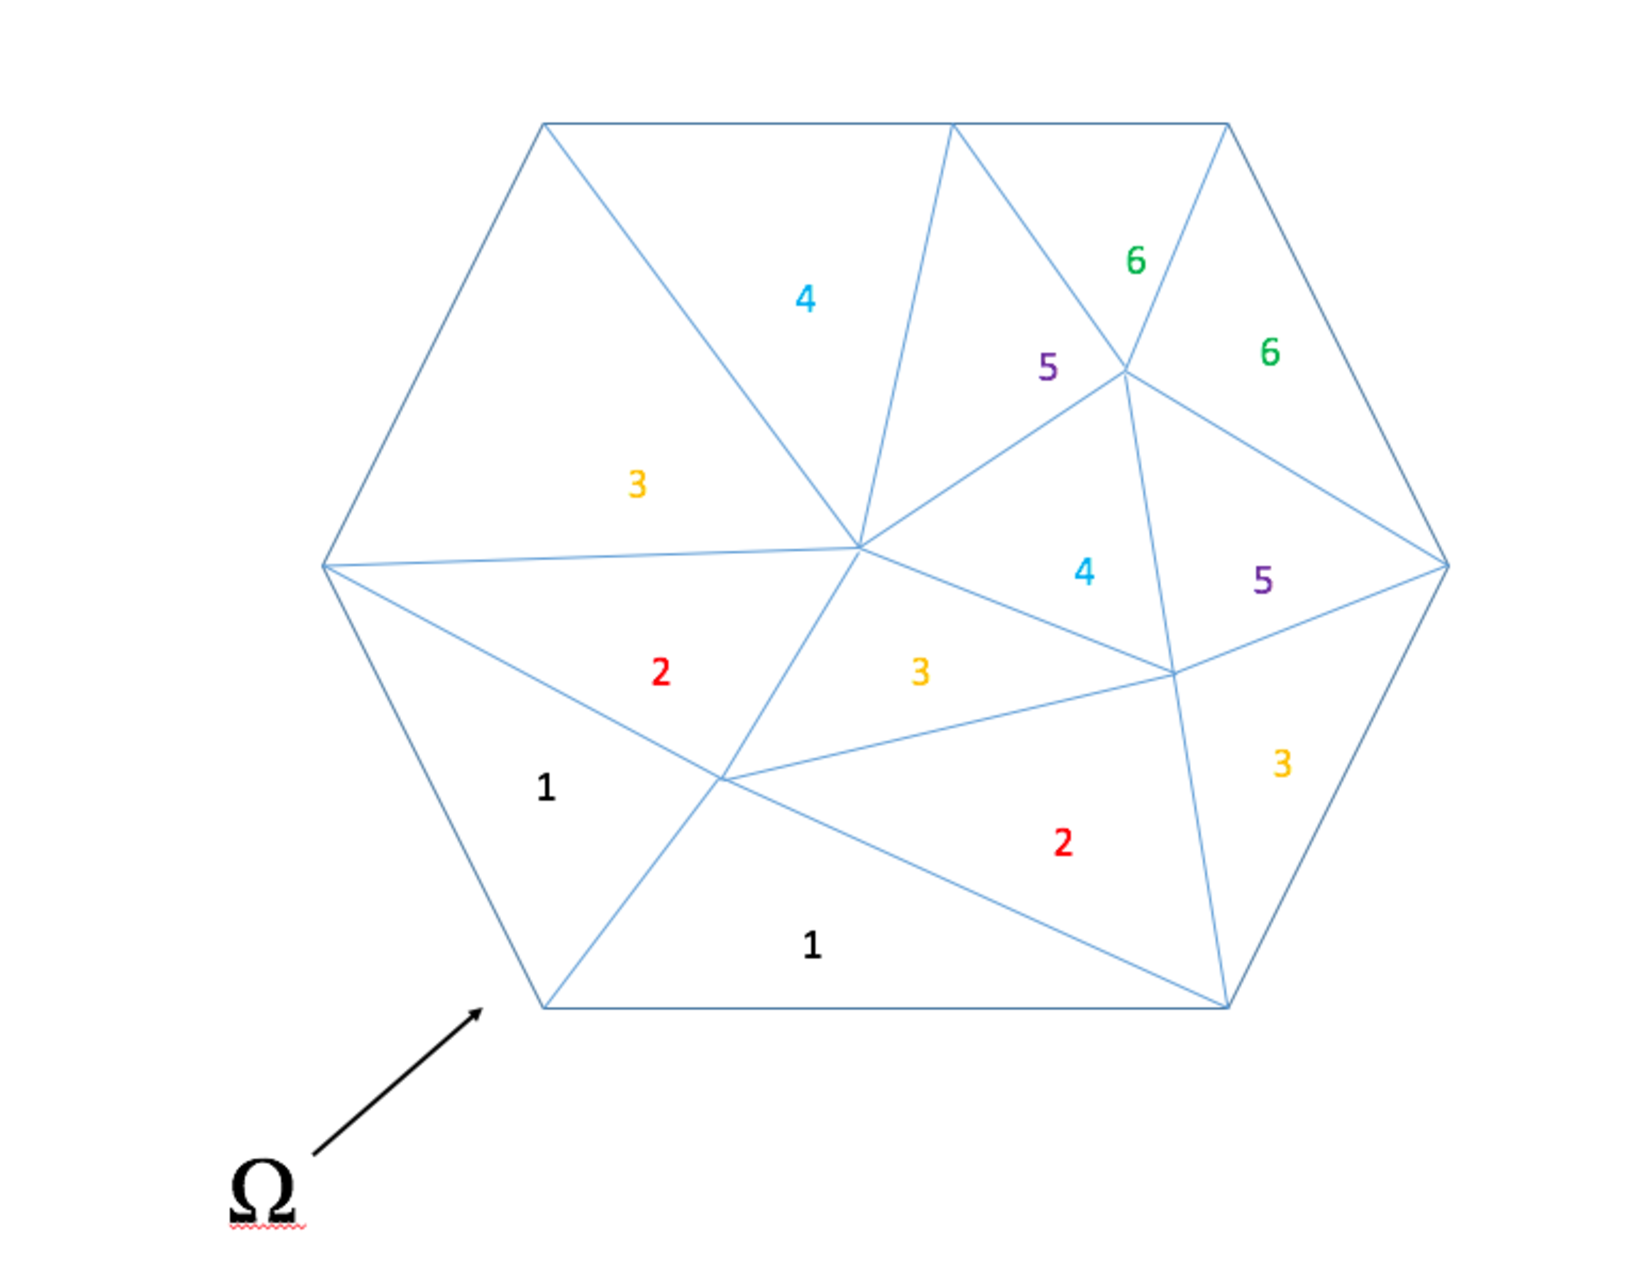
\includegraphics[scale = 0.27]{figures/UnstructureMesh.pdf}
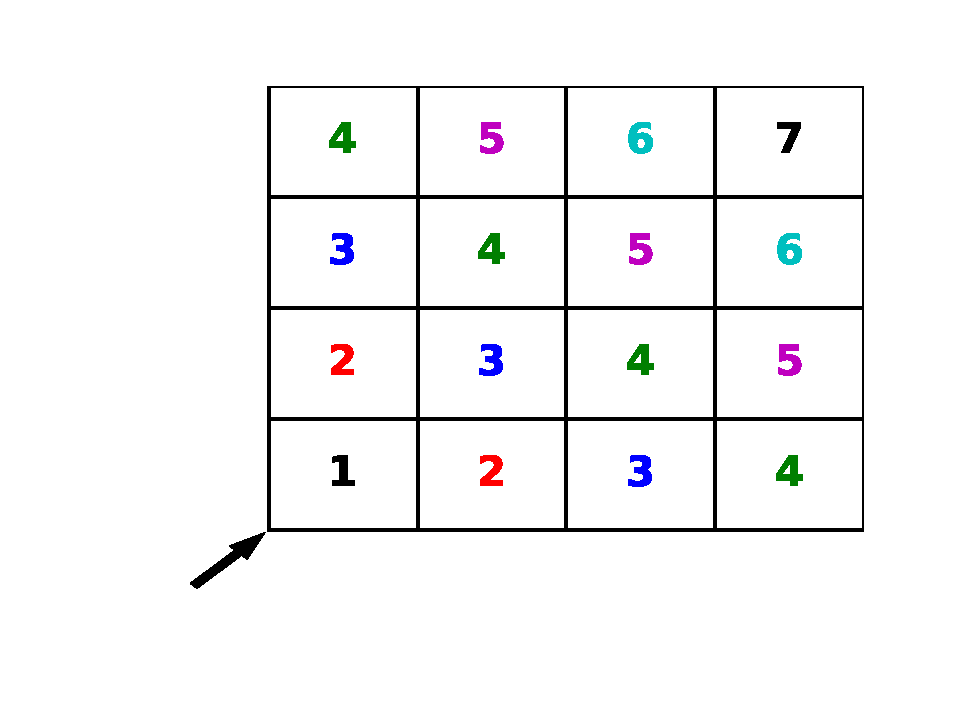
\includegraphics[scale = 0.27]{figures/StructuredMesh.pdf}
\captionof{figure}{A demonstration of a sweep on a structured and unstructured mesh. }
\label{sweeps}
\end{minipage}
\smallskip

The number in each cell represents the order in which the cells are solved. All cells must receive the solution downwind from them before solving for their own solution. This dependency can be represented and stored as a task dependence graph, shown in Fig. \ref{tdg}.

\noindent\begin{minipage}{\textwidth}
\centering
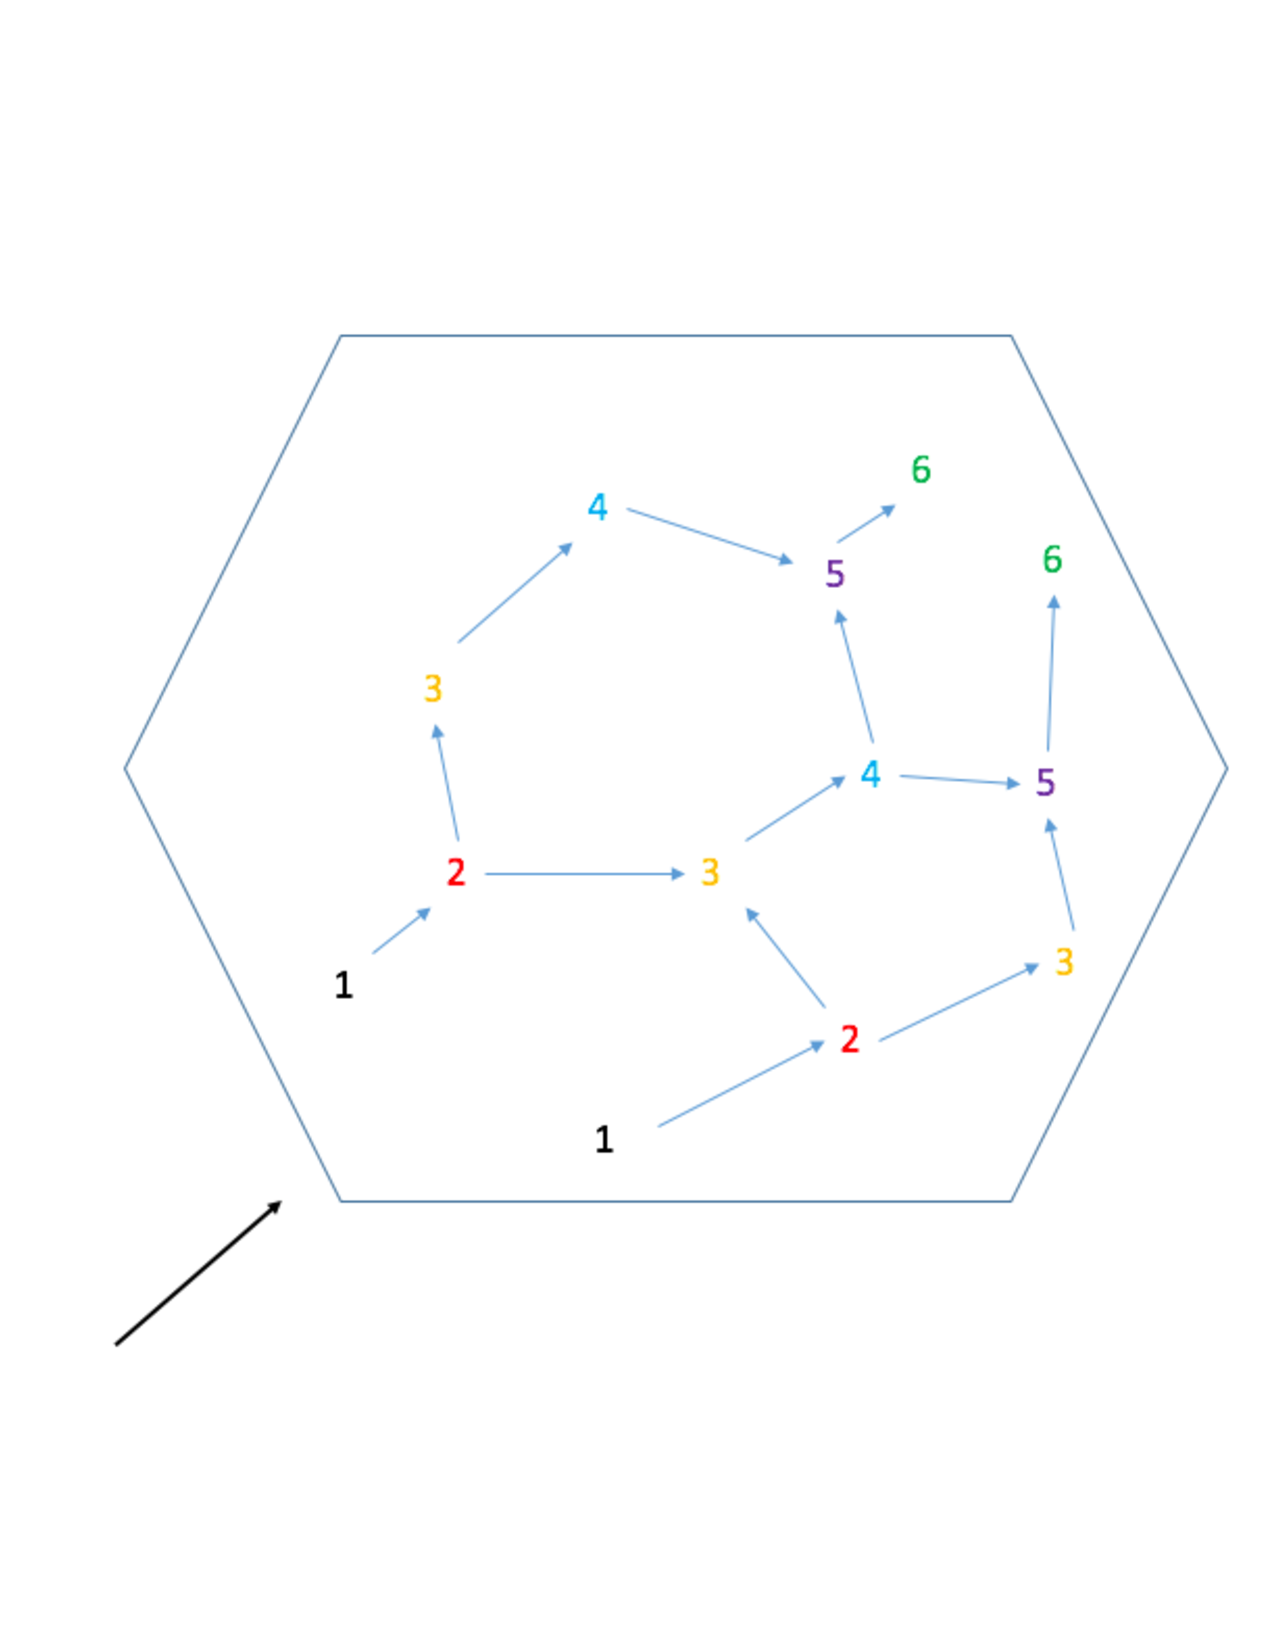
\includegraphics[scale = 0.5,trim = 0cm 3.5cm 0cm 3cm,clip]{figures/tdg.pdf}
\captionof{figure}{A task dependence graph of the unstructured mesh example in Fig. \ref{sweeps}.}
\label{tdg}
\end{minipage}
\smallskip

%%%%Parallel Transport Sweep


%\pagestyle{plain} % No headers, just page numbers
%\pagenumbering{arabic} % Arabic numerals
%\setcounter{page}{8}


\chapter{\uppercase {Parallelization of Transport Sweeps}}
\label{ch:transportsweeps}

As mentioned in the previous section, a transport sweep is set up by overlaying a domain with a finite element mesh. The sweep then solves the transport equation cell by cell using a discontinuous finite element approach. The order of which cell to solve first is given by a task dependence graph, as shown in Fig. \ref{tdg}. The transport sweep can be solved in parallel in order to obtain the solution faster, as well as distribute the memory to many processors for memory intensive cases. In PDT, a transport sweep can be performed on a structured Cartesian mesh, and the work proposed utilizes transport sweeps on an unstructured mesh. Performing a transport sweep on an unstructured mesh presents two big challenges: performing a transport sweep on a massively parallel scale in an efficient manner and keeping non-concave sub-domains due to the nature of the transport sweep itself. PDT has already proven the ability to perform massively parallel transport sweeps on structured meshes. As part of previous efforts in PDT, researchers have come to outline three important properties for parallel sweeps. 

A parallel sweep algorithm is defined by three properties\cite{mpadams2013} :
\begin{itemize}
\item partitioning: dividing the domain among available processors
\item aggregation: grouping cells, directions, and energy groups into tasks
\item scheduling: choosing which task to execute if more than one is available
\end{itemize}

The basic concepts of parallel transport sweeps, partitioning, aggregation, and scheduling, are most easily described in the context of a structured transport sweep. A structured transport sweep takes place on a Cartesian mesh. Furthermore, the work proposed utilizes aspects of the structured transport sweep.

If $M$ is the number of angular directions per octant, $G$ is the total number of energy groups, and $N$ is the total number of cells, then the total fine grain work units is $8MGN$. The factor of 8 is present as $M$ directions are swept for all 8 octants of the domain. The finest grain work unit is the calculation of a single direction and energy groups unknowns in a single cell, or $\psi_{m,g}$ for a single cell.

In a regular grid, we have the  number of cells in each Cartesian direction: $N_x, N_y, N_z$. These cells are aggregated into ``cellsets''. If $M$ is the total number of angular directions, $G$ is the total number of energy groups, and $N$ is the total number of cells, then the total fine grain work units is $8MGN$. The factor of 8 is present as $M$ directions are swept for all 8 octants of the domain. The finest grain work unit is the calculation of a single direction and energy groups unknowns in a single cell, or $\psi_{m,g}$ for a single cell.

Fine grain work units are aggregated into coarser-grained units called \textit{tasks}. A few terms are defined that describe how each variable is aggregated.
\begin{itemize}
\item $A_x = \frac{N_x}{P_x}$, where $N_x$ is the number of cells in $x$ and $P_x$ is the number of processors in $x$
\item $A_y = \frac{N_y}{P_y}$, where $N_y$ is the number of cells in $y$ and $P_y$ is the number of processors in $y$
\item $N_g = \frac{G}{A_g}$
\item $N_m = \frac{M}{A_m}$
\item $N_k = \frac{N_z}{P_z A_z}$
\item $N_k A_x A_y A_z = \frac{N_x N_y N_z}{P_x P_y P_z}$
\end{itemize}

It follows that each process owns $N_k$ cell-sets (each of which is $A_z$ planes of $A_x A_y$ cells), $8N_m$ direction-sets, and $N_g$ group-sets for a total of $8N_m N_g N_k$ tasks.

One task contains $A_x A_y A_z$ cells, $A_m$ directions, and $A_g$ groups. Equivalently, a task is the computation of one cellset, one groupset, and one angleset. One task takes a stage to complete.  This is particularly important when comparing sweeps to the performance models. 

Equation ~\eqref{paralleleff} approximately defines parallel sweep efficiency. This can be calculated for specific machinery and partitioning parameters by substituting in values calculated using Eqs.~\eqref{nfill},~\eqref{nidle}, and ~\eqref{ntasks}.
\begin{equation}\label{paralleleff}
\begin{split}
\epsilon &= \frac{T_{\text{task}} N_{\text{tasks}}}{[N_{\text{stages}}] [T_{\text{task}} + T_{\text{comm}}]} \\
            &=\frac{1}{[1+\frac{N_{\text{idle}}}{N_{\text{tasks}}}][1 + \frac{T_{\text{comm}}}{T_{\text{task}}}]}
\end{split}
\end{equation}

Equations ~\eqref{Tcomm} and \ref{Ttask} show how $T_{\text{comm}}$ and $T_{\text{task}}$ are calculated:
\begin{equation}
T_{\text{comm}} = M_L T_{\text{latency}} + T_{\text{byte}} N_{\text{bytes}}
\label{Tcomm}
\end{equation}
\begin{equation}
T_{\text{task}} = A_x A_y A_z A_m A_g T_{\text{grind}}
\label{Ttask}
\end{equation}
where $T_{\text{latency}}$ is the message latency time, $T_{\text{byte}}$ is the time required to send one byte of message, $N_{\text{bytes}}$ is the total number of bytes of information that a processor must communicate to its downstream neighbors at each stage, and $T_{\text{grind}}$ is the time it takes to compute a single cell, direction, and energy group. $M_L$ is a latency parameter that is used to explore performance as a function of increased or decreased latency. If a high value of $M_L$ is necessary for the performance model to match computational results, improvements should be made in code implementation.

\section{KBA Partitioning for Structured Grids}

Several parallel transport sweep codes use KBA partitioning in their sweeping, such as Denovo \cite{denovo} and PARTISN \cite{partisn}. The KBA partitioning scheme and algorithm was developed by Koch, Baker, and Alcouffe \cite{partisn}.

The KBA algorithm traditionally chooses $P_z = 1, A_m = 1, G = A_g = 1, A_x = N_x/P_x, A_y = N_y/P_y$, with $A_z$ being the selectable number of z-planes to be aggregated into each task. With $N_k = N_z/A_z$, each processor performs $N_{\text{tasks}} = 8MN_k$ tasks. With the KBA algorithm, $2MN_k$ tasks are pipelined from a given corner of the 2D processor layout. The far corner processor remains idle for the first $P_x + P_y - 2 $ stages, which means that an octant-pair (or quadrant) sweep completes in $2MN_k + P_x + P_y - 2$ stages. If an octant-pair sweep does not begin until the previous pair's finishes, the full sweep requires $8MN_k + 4(P_x+P_y-2)$ stages, which means the KBA parallel efficiency is:
\begin{equation}
\varepsilon_{KBA} = \frac{1}{[1+\frac{4(P_x+P_y-2)}{8MN_k}][1+\frac{T_{\text{comm}}}{T_{\text{task}}}]}
\label{eKBA}
\end{equation}

\tcr{in the next section, you talk about stages, minimum number of stages to reach
the center-most proc, ..., it would be good that to discuss KBA and PDT sweeps with as much as possible the same language. Add a few things here to allow for an easier comparison with the PDT text below}

%%%%%%%%%%%%%%%%%%%%%%%%%%%%%%%%%%%%%%%%%%%%%%%%%%%%%%%%%%%%%%%%%%%%%
\section{The Structured Transport Sweep in PDT}
%%%%%%%%%%%%%%%%%%%%%%%%%%%%%%%%%%%%%%%%%%%%%%%%%%%%%%%%%%%%%%%%%%%%%
The minimum possible number of stages for given partitioning parameters $P_i$ and $A_j$ is $2 N_{\text{fill}}+N_{\text{tasks}}$. $N_{\text{fill}}$ is both the minimum number of stages before a sweepfront can reach the center-most processors and the number needed to finish a direction's sweep after the center-most processors have finished. Equations~\eqref{nfill}, ~\eqref{nidle}, and~\eqref{ntasks} define $N_{\text{fill}}$, $N_{\text{idle}}$, and $N_{\text{tasks}}$:
\begin{equation}
N_{\text{fill}} = \frac{P_x + \delta_x}{2} - 1 + \frac{P_y + \delta_y}{2} - 1 + N_k (\frac{P_z + \delta_z}{2} - 1)
\label{nfill}
\end{equation}
\begin{equation}
N_{\text{idle}} = 2 N_{\text{fill}}
\label{nidle}
\end{equation}
\begin{equation}
N_{\text{tasks}} = 8 N_m N_g N_k
\label{ntasks}
\end{equation}
where $\delta_u$ is 1 for $P_u$ odd, and 0 for $P_u$ even.

\tcr{next, you start discussing volumetric overladed and non-overloaded but it feels that the discussion above doesn't naturally lead to this. Can you explain the logic a bit more. 
First, why do you call it volumetric? Are they not all volumetric? To me, volumetric also implies no long skinny columns ... so is this a got term? Also, you give an efficiency in eq. 3.8 but it may not be clear how you compare it to KBA. I feel there is a bit of a mix in between the MC2013 and MC2015 papers of Michael, but try to get the bottom line to be evident.} 
\tcr{Later, you say hybrid-KBA but explain how it is related to the SQO discussion below, I was under the impression hybrid was mainly Pz=2...}

Figure \ref{partitioning} shows three different partitioning schemes used in transport sweeps, KBA (which is defined in the previous section), volumetric non-overloaded, and volumetric overloaded. Volumetric non-overloaded requires that all cells owned by a processor are contiguous, where as volumetric non-overloaded partitioning does not have this restriction.  

\noindent\begin{minipage}{\textwidth}
\centering
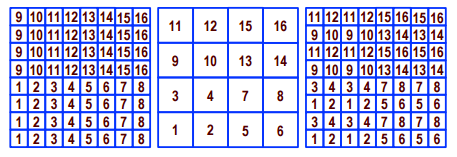
\includegraphics[scale = 1]{figures/Partitioning.png}
\captionof{figure}{Three different partitioning schemes in 2D, from left to right: KBA, volumetric non-overloaded, and volumetric overloaded.}
\label{partitioning}
\end{minipage}
\smallskip

The overloaded volumetric partitioning proceeds as follows:

\begin{enumerate}
\item In a 2D (3D) domain, cellsets are divided into 4 (8) spatial quadrants (octants), with an equal number of cellsets in each  SQO (SQO is defined as a spatial quadrant or octant).
\item Assign 1/4 of the processors (1/8) in 3D to each SQO. 
\item Choose the individual overload factors $\omega_x, \omega_y, \text{and } \omega_z$ and individual processor counts $P_x, P_y, \text{and }P_z$, such that $\omega_x \omega_y \omega_z = \omega_r$ and $P_x P_y P_z = P$, with all $P_u$ even. $\omega_u$ is defined as the number of cellsets assigned to each $P_u$.
\item An array of $\omega_x\cdot\omega_y\cdot\omega_z$ ``tiles'' in each SQO. Each tile is an array of $1/2 P_x \cdot 1/2 P_y \cdot 1/2 P_z$ cellsets. These cellsets are mapped one-to-one to the $1/2 P_x \cdot 1/2 P_y \cdot 1/2 P_z$ processors assigned to the SQO, using the same mapping in each tile.
\end{enumerate}
Each tile has a logically identical layout of cellsets, and each processor owns exactly one cellset in each tile in its SQO. This makes each processor responsible for $\omega_r$ cellsets.

In order to properly outline the optimal scheduling rules, the variables $X,Y, \text{and } Z$ are defined as $P_u/2$ for each respective direction $u = x,y,z$. This splits up the processor layout into octants, where each processor has an index $(i,j,k)$ determining where it is in the layout. Tiles are also indexed and referred to in the same way with the notation $T(i,j,k)$. 

The optimal scheduling algorithm rules are as follows:
\begin{enumerate}
\item If $i \leq X$, then tasks with $\Omega_x > 0$ have priority, while for $i > X$, tasks with $\Omega_x < 0$ have priority.
\item If multiple ready tasks have the same sign on $\Omega_x$, apply rule 1 to $j,Y,\Omega_y$.
\item If multiple ready tasks have the same sign on $\Omega_x$ and $\Omega_y$, apply rule 1 to $k,Z, \Omega_z$. 
\item If multiple tasks are ready in the same octant, then priority goes to the cellset for which the priority octant has greatest downstream depth.
\item If multiple ready tasks are in the same octant and have the same downstream depth of graph in $x$, then priority goes to the cellset for which the priority octant has greatest downstream depth of graph in $y$.
\item If multiple ready tasks are in the same octant and have the same downstream depth of graph in $x$ and $y$, then priority goes to the cellset for which priority octant has greatest depth of graph in $z$.
\end{enumerate}
This ensures that each SQO orders the octants: the one it can start right away ($A$), three that have one sign difference from $A (B,C,$ and $D)$, three that have two sign differences ($\bar D, \bar C, \bar B$), and one in opposition to its primary ($\bar A$). For example, if octant $A$ is octant $(+x, +y, +z)$, then it's secondary octants (only one sign change at a time) would be octants $(-x, +y, +z)$, $(+x,-y,+z)$ and $(+x,+y,-z)$.

There are three constraints in order to achieve the optimal stage count. In these constraints, $M = \omega_g \omega_m/8$, which is the number of tasks per octant per cellset.
\begin{enumerate}
\item $ M \geq 2(Z-1)$
\item $\omega_z M \geq 2(Y-1)$
\item If $\omega_x > 1$, then $\omega_y \omega_z M \geq X$
\end{enumerate}
Constraint 1 ensures that there is no idle time between a processor finishing an octant's work in one tile and beginning that octant's work on the next tile in the same tile-column; processor $P(1,Y,1)$ finishing its tile $T(1,\omega_y,1)$ octant $C$ work and beginning its octant $B$ work; processor $P(X,1,1)$ finishing its tile $T(\omega_x,1,1)$ octant $D$ work and beginning its octant $B$ work. Constraint 2 ensures that there is no idle time time between a processor finishing an octant's work for one $z$ column of tiles and beginning that octant's work on the next column; processor $P(X,1,1)$ finishing its tile $T(\omega_x,1,1)$ octant D work available to it and beginning its octant $C$ work. Constraint 3 ensures that there is no idle time between a processor finishing an octant's work for one $yz$ plane of tiles and beginning that octant's work in the next plane.

As a result of these constraints, there is no idle time for a variety of situtations. At large processor counts, the product $\omega_m \omega_g$ must be large, which requires $N_m N_g$ be large. This means that a weak scaling series refined only in space, but only coarsely refined in angle and energy, will eventually fail the constraints.

The optimal efficiency formula changes slightly from the KBA and hybrid KBA partitioning method in order to account for the overload factors. The only change is in the $\frac{N_{idle}}{N_{tasks}}$ term, as shown in Eq. ~\eqref{overloadpartitioning}. 
\begin{equation}
\varepsilon_{opt} = \frac{1}{[1+\frac{P_x+P_y+P_z-6}{\omega_g \omega_m \omega_r}][1+\frac{T_{\text{comm}}}{T_{\text{task}}}]}
\label{overloadpartitioning}
\end{equation}


%%%%%%%%%%%%%%%%%%%%%%%%%%%%%%%%%%%%%%%%%%
\section{The Unstructured Transport Sweep}
%%%%%%%%%%%%%%%%%%%%%%%%%%%%%%%%%%%%%%%%%%
In an unstructured mesh, the number of cells cannot be described in the same way as an unstructured mesh. In PDT specifically we initially subdivide the domain into subsets, which are just rectangular subdomains. Within each subset, an unstructured mesh is created. This creates a pseudo-regular grid. These subsets become the $N_x, N_y, N_z$ equivalent for an unstructured mesh. The spatial aggregation in a PDT unstructured mesh is done by aggregating subsets into cellsets. 

While the structured PDT transport sweep has scaled well out to 750,000 cores, similar levels of parallel scaling have not been achieved using unstructured sweeps yet. Pautz proposed a new list scheduling algorithm has been constructed for modest levels of parallelism (up to 126 processors)\cite{Pautz} .

There are three requirements for a sweep scheduling algorithm to have. First, the algorithm should have low complexity, since millions of individual tasks are swept over in a typical problem. Second, the algorithm should schedule on a set of processors that is small in comparison to the number of tasks in the sweep graph. Last, the algorithm should distribute work in the spatial dimension only, so that there is no need to communicate during the calculation of the scattering source. 

Here is the pseudocode for the algorithm:

\begin{verbatim}
Assign priorities to every cell-angle pair
Place all initially ready tasks in priority queue
While (uncompleted tasks)
    For i=1,maxCellsPerStep
       Perform task at top of priority queue
       Place new on-processor tasks in queue
    Send new partition boundary data
    Receive new partition boundary data
    Place new tasks in queue 
\end{verbatim}

An important part of the algorithm above is the assigning priorities to tasks. Specialized prioritization heuristics generate partition boundary data as rapidly as possible in order to minimize the processor idle time. 

Nearly linear speedups were obtained on up to 126 processors\cite{Pautz}. Further work is being done for scaling to thousands of processors. 

\subsection{Cycle Detection}

A cycle is a loop in a directed graph and they can occur commonly in unstructured meshes. However, they do not exist in 2D triangular extruded problems and, because our domain partitioning is convex, arbitrary degenerate polygons appearing on subdomain boundaries will not produce cycles. Even though they are not applicable to this application of unstructured transport sweeps, they are discussed here for completeness.

Cycles can cause hang time in the problem, as a processor will wait for a message that might will never come. This means that the computation for one or more elements will never be completed. The solution to this is to ``break'' any cycles that exist by removing an edge of the task dependence graph (TDG). Old flux information is used on a particular element face in the domain. Most of the time, the edge removed is oriented obliquely with respect to the radiation direction. 

Algorithms for finding cycles are called \textit{cycle detection} algorithms. This must be done efficiently in parallel, both because the task dependence graph is distributed and because the finite element grid may be deforming every timestep and changing the associated TDG.

Cycle detection utilizes two operations: trim and mark. Trimming identifies and discards elements which are not in cycles. At the beginning of cycle detection, graphs are trimmed in the downwind direction, then the remaining graphs are trimmed in the upwind direction. A pivot vertex is then selected in each graph. Graph vertices are then marked as upwind, downwind, or unmarked. Then, if any vertices are both upwind and downwind, the cycle is these vertices plus the pivot vertex. An edge is removed between 2 cycle vertices, and 4 new graphs are created: a new cycle, the upwind vertices without the cycle, the downwind vertices without the cycle, and a set of unmarked vertices. This recursively continues until all cycles are eliminated.
%\pagestyle{plain} % No headers, just page numbers
%\pagenumbering{arabic} % Arabic numerals
%\setcounter{page}{1}

\chapter{\uppercase {Motivation and Methods}}
\label{ch:motivation}

The capability for PDT to generate and run on an unstructured mesh is important because it allows us to run problems without having to conform our mesh to the problem as much. The idea is to have a logically Cartesian grid (creating orthogonal ``subsets") with an unstructured mesh inside each subset. These logically Cartesian subdomains are obtained using cut planes in 3D and cut lines in 2D. Figure \ref{grid} demonstrates this functionality, with the first two subsets meshed using the Triangle Mesh Generator\cite{triangle}, a 2D mesh generator. 

\noindent\begin{minipage}{\textwidth}
\centering
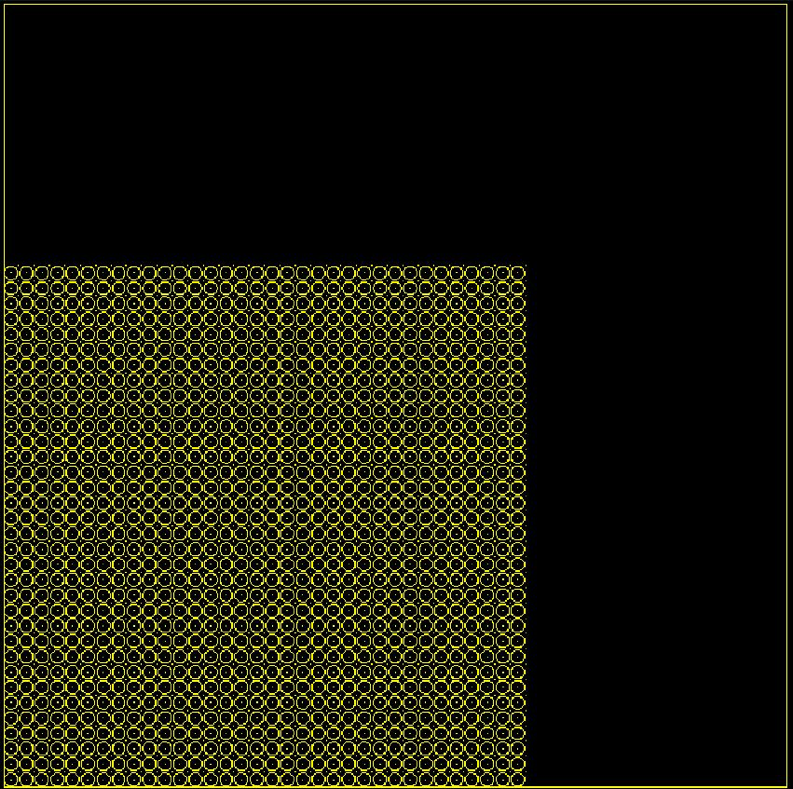
\includegraphics[scale = 0.5]{figures/lattice.png}
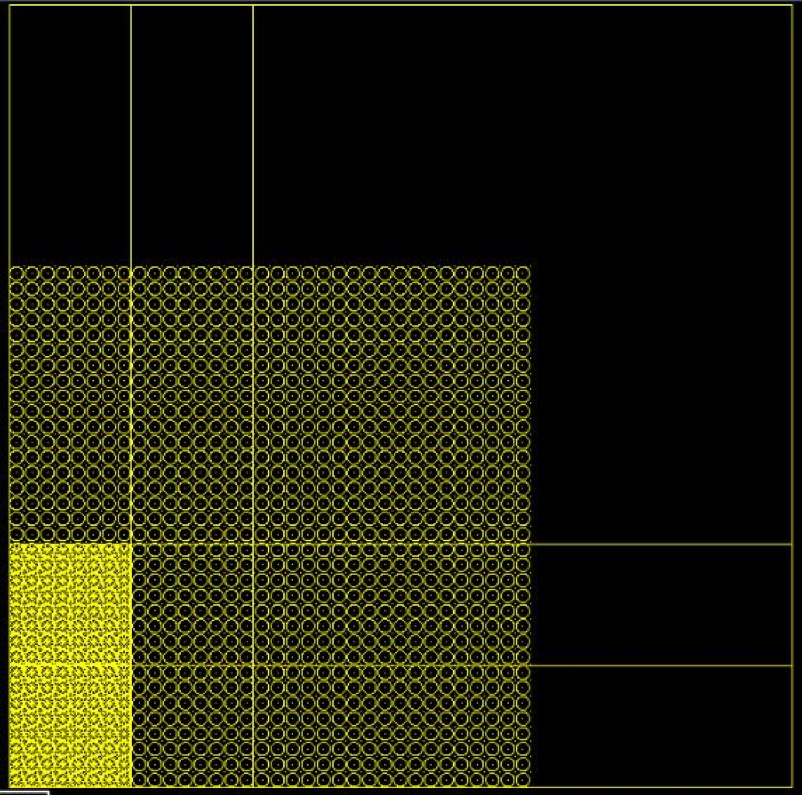
\includegraphics[scale = 0.5]{figures/subsetlattice.png}
\captionof{figure}{A PSLG describing a fuel lattice, and with a orthogonal ``subset" grid imposed on on the PSLG.}
\label{grid}
\end{minipage}
\smallskip

This orthogonal grid is superimposed and each subset is meshed in parallel.  Subsets are now the base structured unit when calculating our parallel efficiency. Discontinuities along the boundary are fixed by ``stitching'' hanging nodes, creating degenerate polygons along subset boundaries. Because PDT's spatial discretization employs Piece-Wise Linear Discontinuous (PWLD) finite element basis functions, there is no problem solving on degenerate polygons. 

When using the unstructured meshing capability in PDT, the input geometry is described by a Planar Straight Line Graph (PSLG). After superimposing the orthogonal grid, a PSLG is created for each subset, and meshed. Because the input's and each subset's PSLG must be described and meshed in 2D, the mesh can be extruded in the $z$ dimension in order to give us the capability to run on 3D problems. Obviously, this is not as good as a unstructured tetrahedral mesh, but for many problems, it is a great capability to have. 

When discussing the parallel scaling of transport sweeps, a load balanced problem is of great importance. A load balanced problem has an equal number of degrees of freedom per processor. Load balancing is important in order to minimize idle time for all processors by equally distributing (as much as possible) the work each processor has to do.  For the purposes of unstructured meshes in PDT, we are looking to ``balance'' the number of cells. Ideally, each processor will be responsible for an equal number of cells. 

If the number of cells in each subset can be reasonably balanced, then the problem is effectively load balanced. The Load Balance algorithm described below details how the subsets will be load balanced. In summary, the procedure of the algorithm involves moving the initially user specified $x$ and $y$ cut planes, re-meshing, and iterating until a reasonably load balanced problem is obtained.  Equation \ref{metric_def} shows the equation for calculating the load balancing metric, which dictates how balanced or unbalanced the problem is.
\begin{equation}
f =\underset{ij}{\text{max}}(N_{ij})/\frac{N_{tot}}{I\cdot J},
\label{metric_def}
\end{equation}
where $f$ is the load balance metric, $N_{ij}$ is the number of cells in subset $i,j$, $N_tot$ is the global number of cells in the problem, and $I$ and $J$ are the total number of in the x and y direction, respectively. The metric is a measure of the maximum number of cells per subset divided by the average number of cells per subset.

\noindent\begin{minipage}{\textwidth}
\textbf{Load Balance:} A load balancing algorithm that equalizes the number of triangles per subset. \\
\rule{\textwidth}{0.4pt}
\begin{algorithmic}
\STATE  $I,J$ subsets specified by user
\STATE Mesh all subsets
\STATE  $N_{tot} = $ total number of triangles
\STATE  $N_{ij} = $ number of triangles in subset $ij$
\STATE $f =\underset{ij}{\text{max}}(N_{ij})/\frac{N_{tot}}{I\cdot J}$
\COMMENT {//Check if all subsets meet the tolerance}
\IF {$f < \text{tol}_{\text{subset}}$}
	\STATE DONE with load balancing
\ELSE
	\STATE $f_I = \underset{i}{\text{max}}[\sum_{j} N_{ij}]/\frac{N_{tot}}{I}$
	\STATE $f_J = \underset{j}{\text{max}}[\sum_{i} N_{ij}]/\frac{N_{tot}}{J}$
	\IF {$f_I > \text{tol}_{\text{row}}$}
		\STATE \textbf{Redistribute}($X_i$)
	\ENDIF
	\IF{$f_J > \text{tol}_{\text{col}}$}
		\STATE \textbf{Redistribute}($Y_j$)
	\ENDIF 
	\IF {redistribution occured}
		\STATE REMESH and repeat algorithm
	\ENDIF
\ENDIF
\IF {There is still a discrepancy amongst subsets}
     \STATE Move cutplane segments on the subset level and remesh (may require changes to scheduling algorithm)
\ENDIF
\end{algorithmic}
\rule{\textwidth}{0.4pt}
\end{minipage}

\bigskip

\noindent\begin{minipage}{\textwidth}
\textbf{Redistribute:} A function that moves cut lines in either X or Y. \\
\rule{\textwidth}{0.4pt}
\begin{algorithmic}
\STATE \textbf{Input:}CutLines (X or Y vector that stores cut lines). 
\STATE \textbf{Input:} num\_tri\_row or num\_tri\_col, a pArray containing number of triangles in each row or column 
\STATE \textbf{Input:} The total number of triangles in the domain, $N_{tot}$
\STATE stapl::array\_view num\_tri\_view, over num\_tri\_row/column
\STATE stapl::array\_vew offset\_view
\STATE stapl::partial\_sum(num\_tri\_view) \COMMENT {Perform prefix sum}
\COMMENT {We now have a cumulative distribution stored in offset\_view}
\FOR {$i = 1$ :CutLines.size()-1}

	\STATE vector $<$double$>$ pt1 = [CutLines(i-1), offset\_view(i-1)]
	\STATE vector $<$double$>$ pt2 = [CutLines(i), offset\_view(i)]
	\STATE ideal\_value = $i\cdot \frac{N_{tot}}{\text{CutLines.size()}-1}$
	\STATE X-intersect(pt1,pt2,ideal\_value) \COMMENT{Calculates the X-intersect of the line formed by pt1 and pt2 and the line y = ideal\_value.}
	\STATE CutLines(i) = X-intersect
\ENDFOR
\end{algorithmic}
\rule{\textwidth}{0.4pt}
\end{minipage} 



\chapter{\uppercase {Results}}
\label{ch:results}

The following sections will showcase the metric behavior and convergence for three test cases, solution verification for pure absorber and pure scatterer 2D slab problems, and the new unstructured meshing capability both in 2D and 3D.

\section{Test Cases for Metric Behavior and Convergence}
\label{sec:convergence}
In order to showcase the behavior of the load balancing metric, calculated by Eq. \ref{metric_def} three test cases are presented. Figure \ref{opp} shows the first test case, a 20 cm by 20 cm domain with two pins in opposite corners of the domain. Figure \ref{same} shows the same size domain but with the pins on the same side.These are two theoretically very unbalanced cases, as geometrically there are two features located distantly from each other with an empty geometry throughout the rest of the domain. Figure \ref{lattice} shows a lattice and reflector, which due to it's denser and repeated geometry, theoretically is a more balanced problem. 

A series of 162 inputs was constructed for each case. These inputs are constructed by varying the maximum triangle area from the coarsest possible to 0.01 cm\textsuperscript{2} and the number of subsets, $N$ from 2$\times$2 to 10$\times$10. The tabulated data in Appendix A show the parameters that will change in each input. 

\noindent\begin{minipage}{\textwidth}
\centering
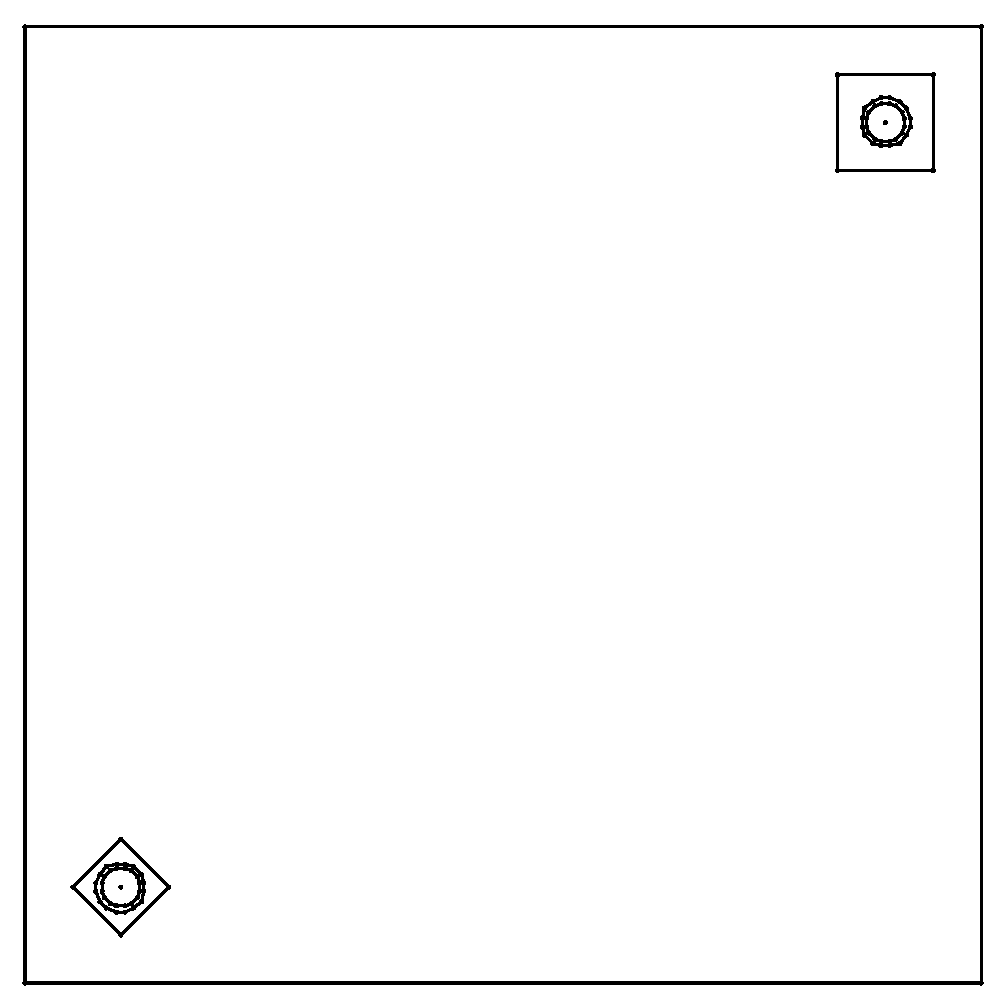
\includegraphics[scale = 0.5]{figures/unbalanced_lattice.eps}
\captionof{figure}{The first test case used in order to test effectiveness and convergence of the load balancing metric.}
\label{opp}
\end{minipage}

\noindent\begin{minipage}{\textwidth}
\centering
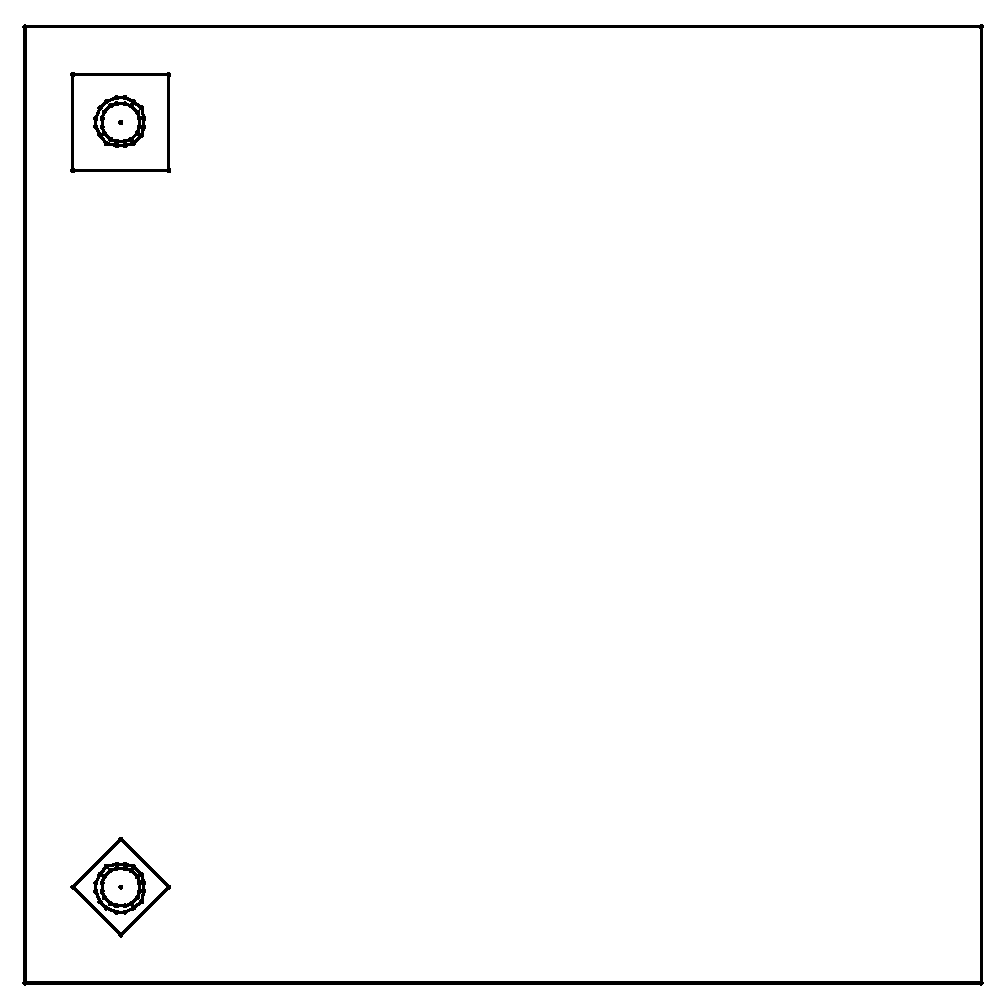
\includegraphics[scale = 0.5]{figures/unbalanced_pins_same_side.eps}
\captionof{figure}{The second test case used in order to test effectiveness and convergence of the load balancing metric.}
\label{same}
\end{minipage}


\noindent\begin{minipage}{\textwidth}
\centering
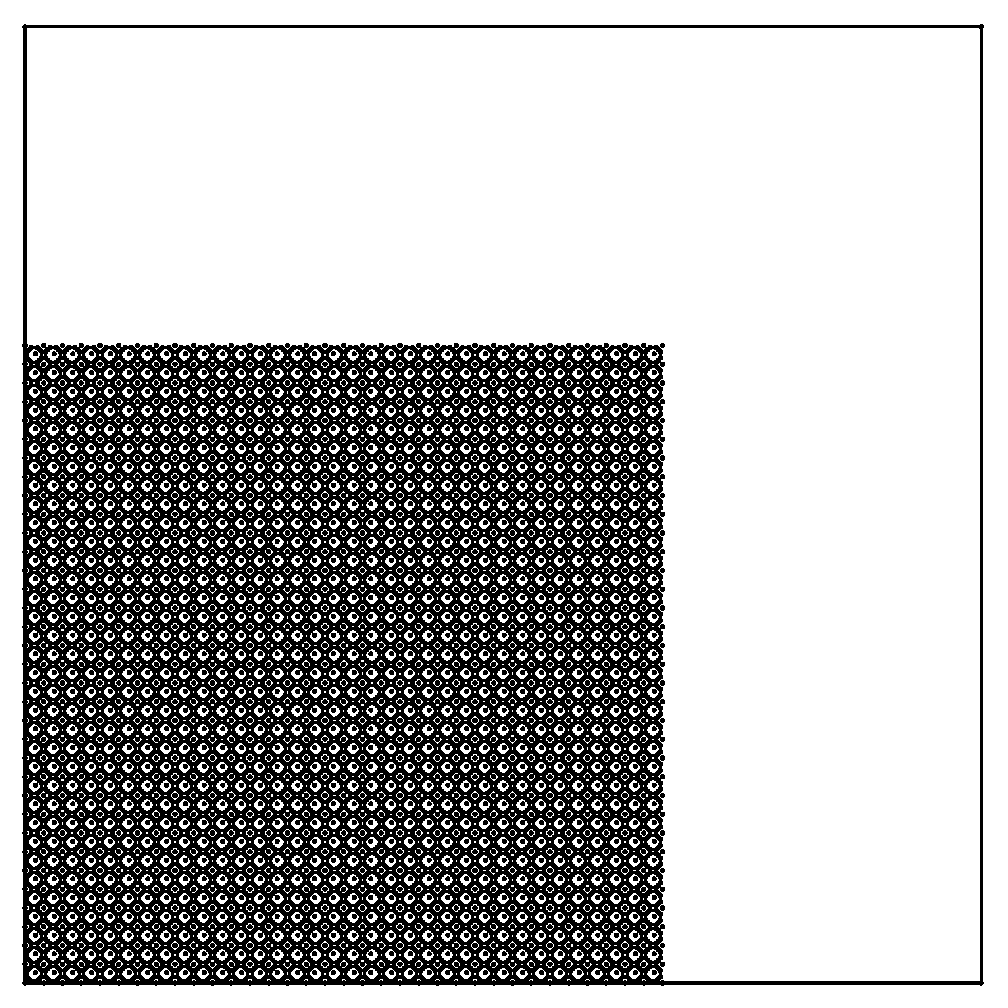
\includegraphics[scale = 0.5]{figures/lattice-12-shifted.eps}
\captionof{figure}{The third test case used in order to test effectiveness and convergence of the load balancing metric.}
\label{lattice}
\end{minipage}

\section{Metric Behavior and Convergence}

For each test case, the 162 input inputs are run twice, once with no load balancing iterations, and once with ten load balancing iterations. The best metric is reported and recorded. Three figures for each test cases are presented below: the first figure will show the metric behavior for no iterations, the second figure will show the metric behavior for each input run with ten load balancing iterations, and the third figure will show a ratio of the ten iteration runs over the no iteration runs.

Figure \ref{oppnoiter} shows the metric behavior for Fig. \ref{opp}. The maximum metric value is 24.7650, and occurs when Fig. \ref{opp} is run with 8x8 subsets and a maximum triangle area of 1.6 cm\textsuperscript{2}. The minimum metric value is 1.0016 and occurs when Fig. \ref{opp} is run with 4x4 subsets and a maximum triangle area of 0.04 cm\textsuperscript{2}. 

\noindent\begin{minipage}{\textwidth}
\centering
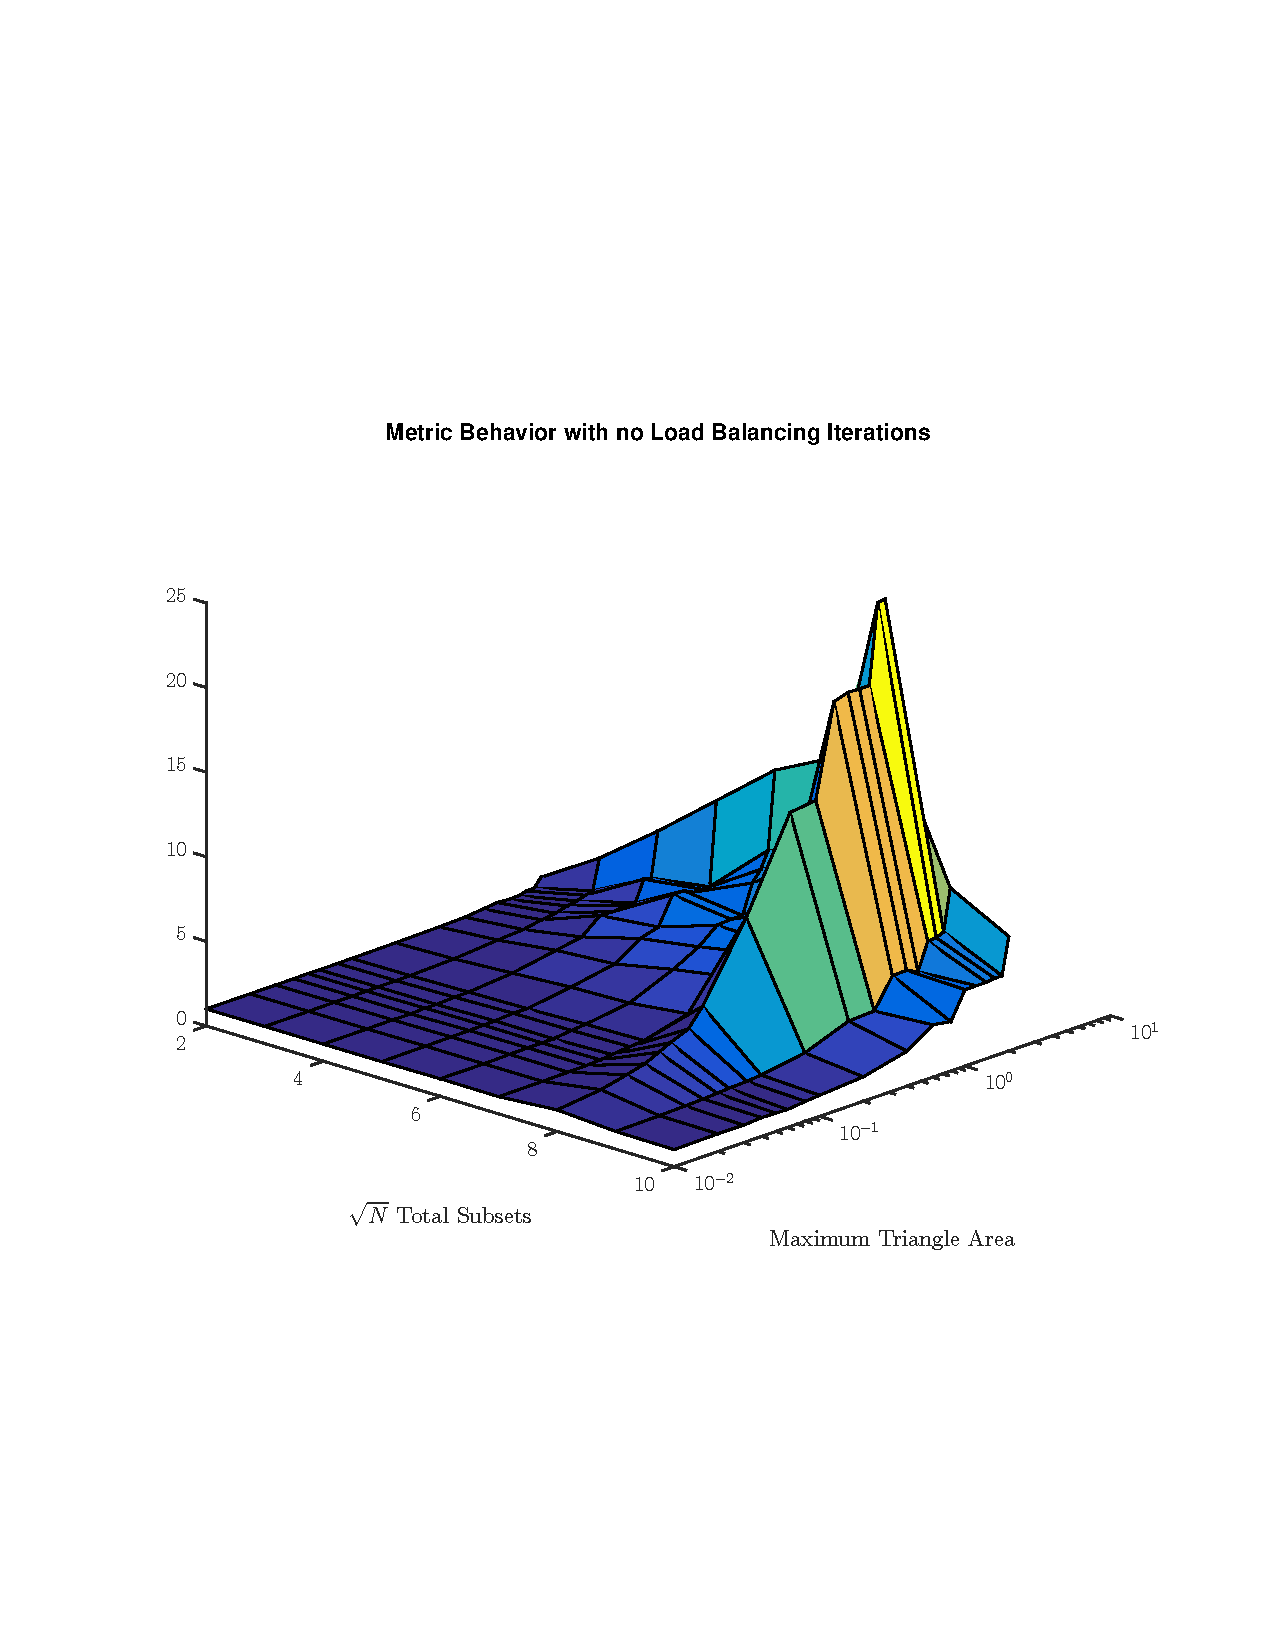
\includegraphics[scale=0.75, trim = 0cm 8cm 0cm 7cm,clip]{figures/OppNoIter.pdf}
\captionof{figure}{The metric behavior of the first test case run with no load balancing iterations.}
\label{oppnoiter}
\end{minipage}
\smallskip

Figure \ref{oppiter} shows the metric behavior for Fig. \ref{opp} after 10 load balancing iterations. The maximum metric value is 5.0538 and occurs when Fig. \ref{opp} is run with 10x10 subsets and a maximum triangle area of 1.2 cm\textsuperscript{2}. The minimum metric value is 1.0017 and occurs when Fig. \ref{opp} is run with 4x4 subsets and a maximum triangle area of 0.04 cm\textsuperscript{2}.

\noindent\begin{minipage}{\textwidth}
\centering
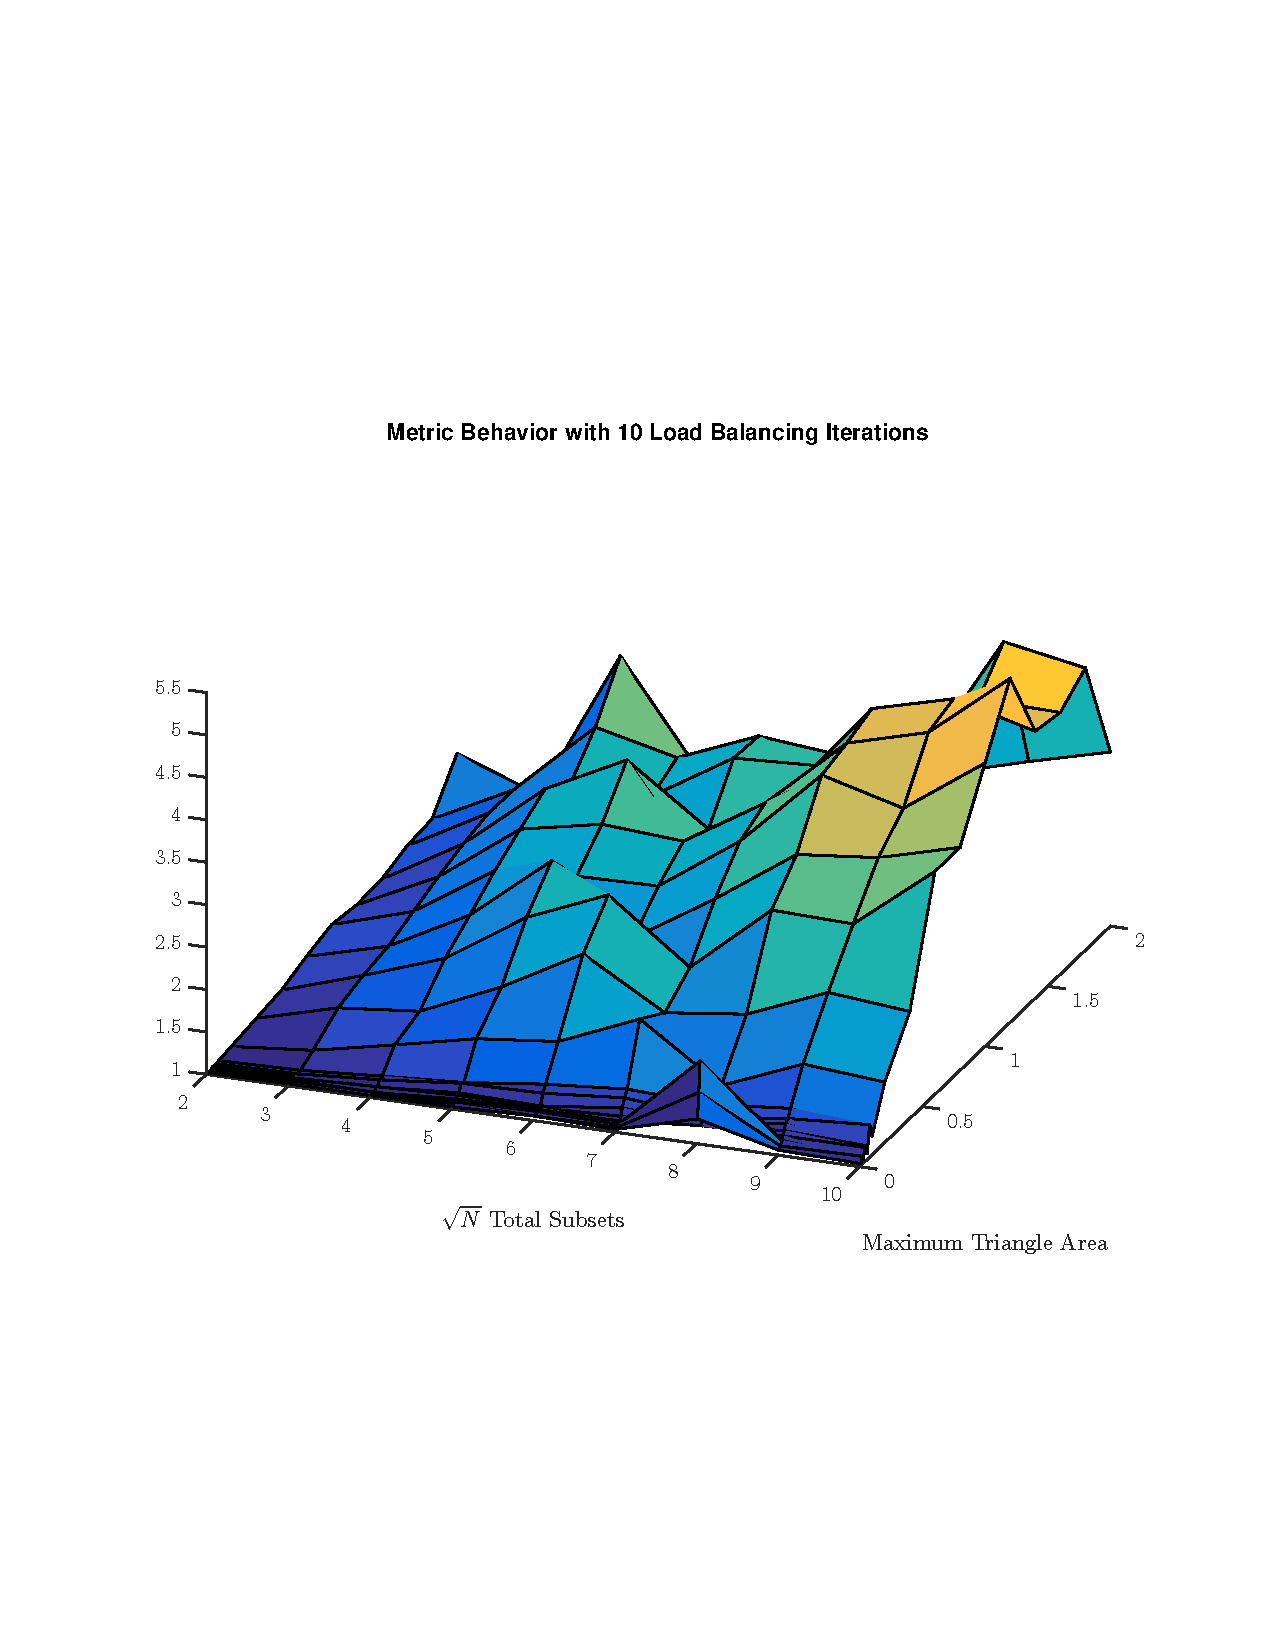
\includegraphics[scale=0.83, , trim = 2cm 6cm 2cm 7cm,clip]{figures/OppIter.pdf}
\captionof{figure}{The metric behavior of the first test case run with 10 load balancing iterations.}
\label{oppiter}
\end{minipage}
\smallskip

Figure \ref{oppdiff} shows the difference in metric behavior for Fig. \ref{opp}. This difference is calculated by dividing the metric with no iterations by the metric with 10 iterations. The maximum improvement has a value of 0.1097 and occurs for Fig. \ref{opp} is run with 8x8 subsets with a maximum triangle area of 1.6 cm\textsuperscript{2}. The minimum improvement has a value of very close to 1.0 and occurs for many of the inputs. 

\noindent\begin{minipage}{\textwidth}
\centering
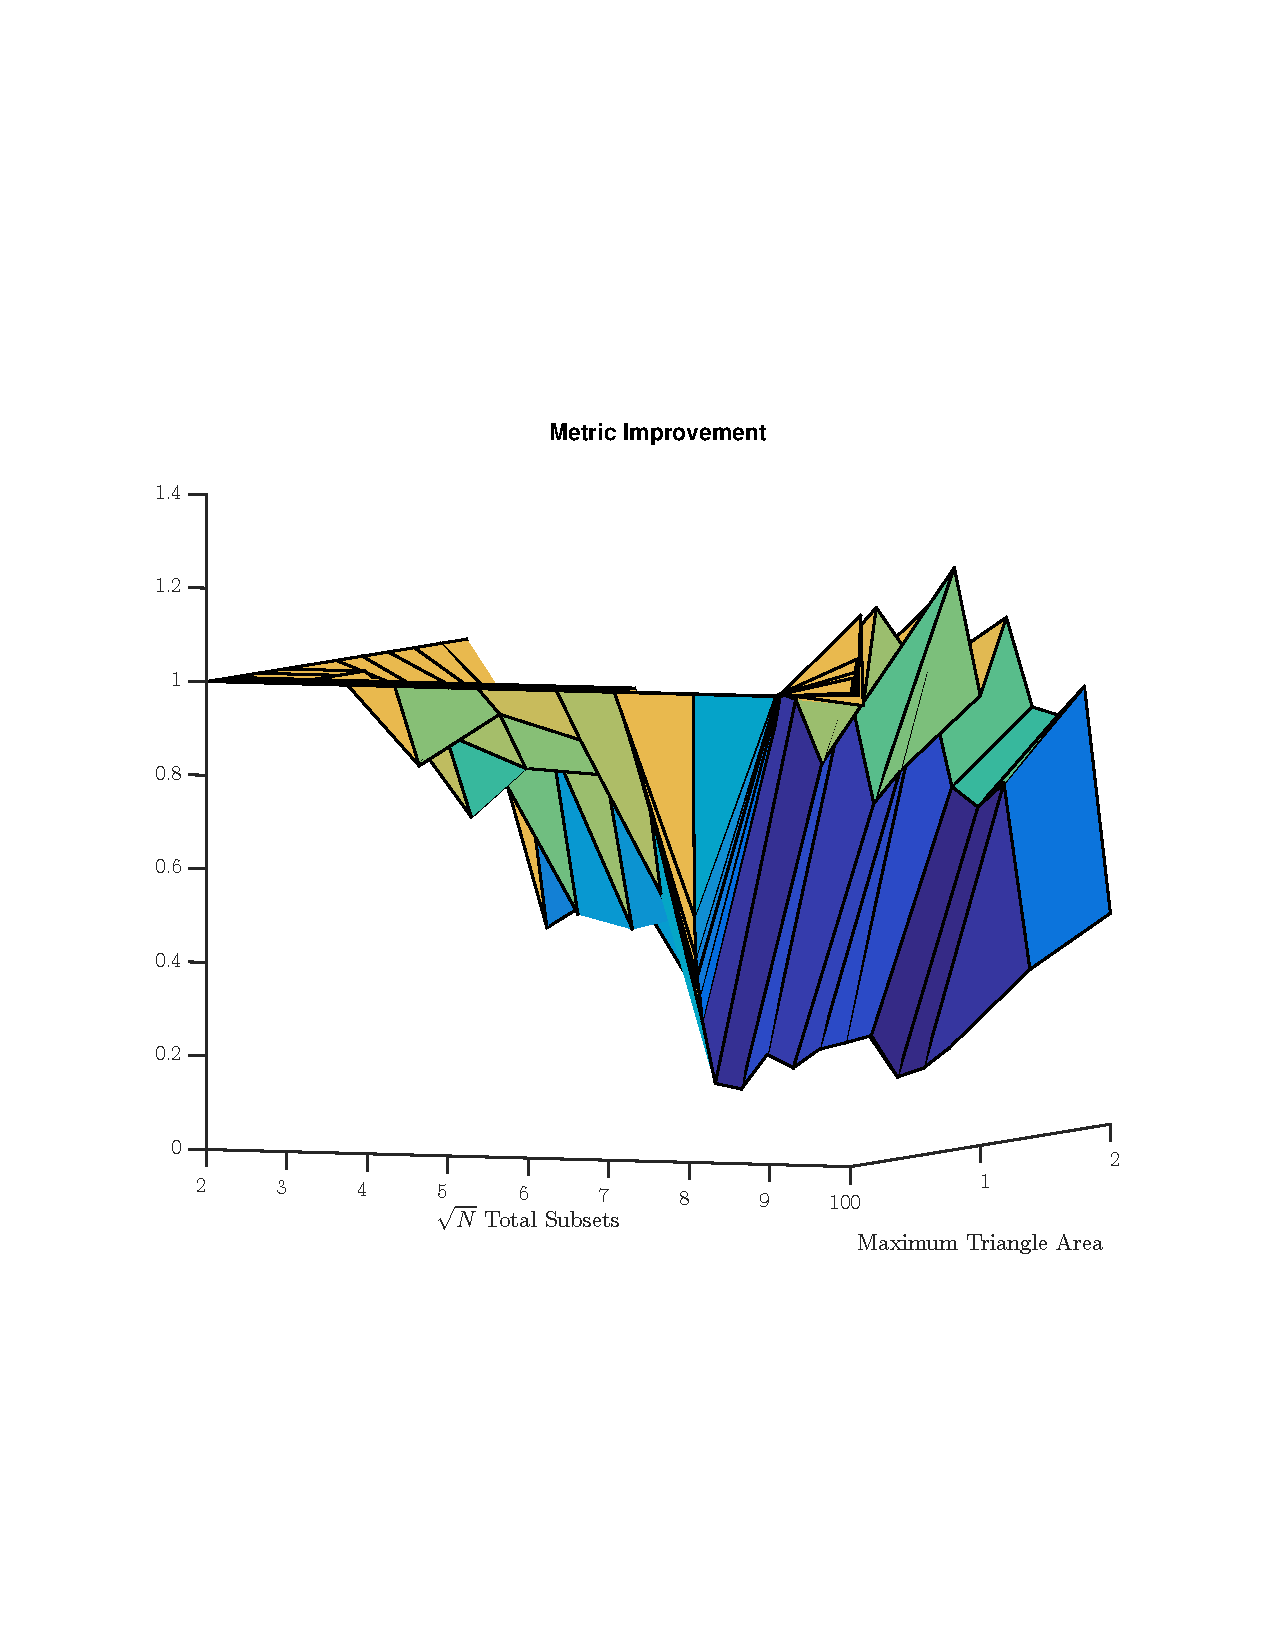
\includegraphics[scale=0.78, trim = 2cm 6cm 2cm 7cm,clip]{figures/OppDiff.pdf}
\captionof{figure}{The difference in metric behavior between no iteration and 10 iterations. The closer the z-value to zero, the better the improvement.}
\label{oppdiff}
\end{minipage}
\smallskip

Figure \ref{samenoiter} shows the metric behavior for Fig. \ref{same}. The maximum metric is 22.6654 and occurs when Fig. \ref{same} is run with 8x8 subsets with a maximum triangle area of 1.8 cm\textsuperscript{2}. The minimum metric is 1.0024 and occurs when Fig. \ref{same} is run with 2x2 subsets with a maximum triangle are of 0.01 cm\textsuperscript{2}.

\noindent\begin{minipage}{\textwidth}
\centering
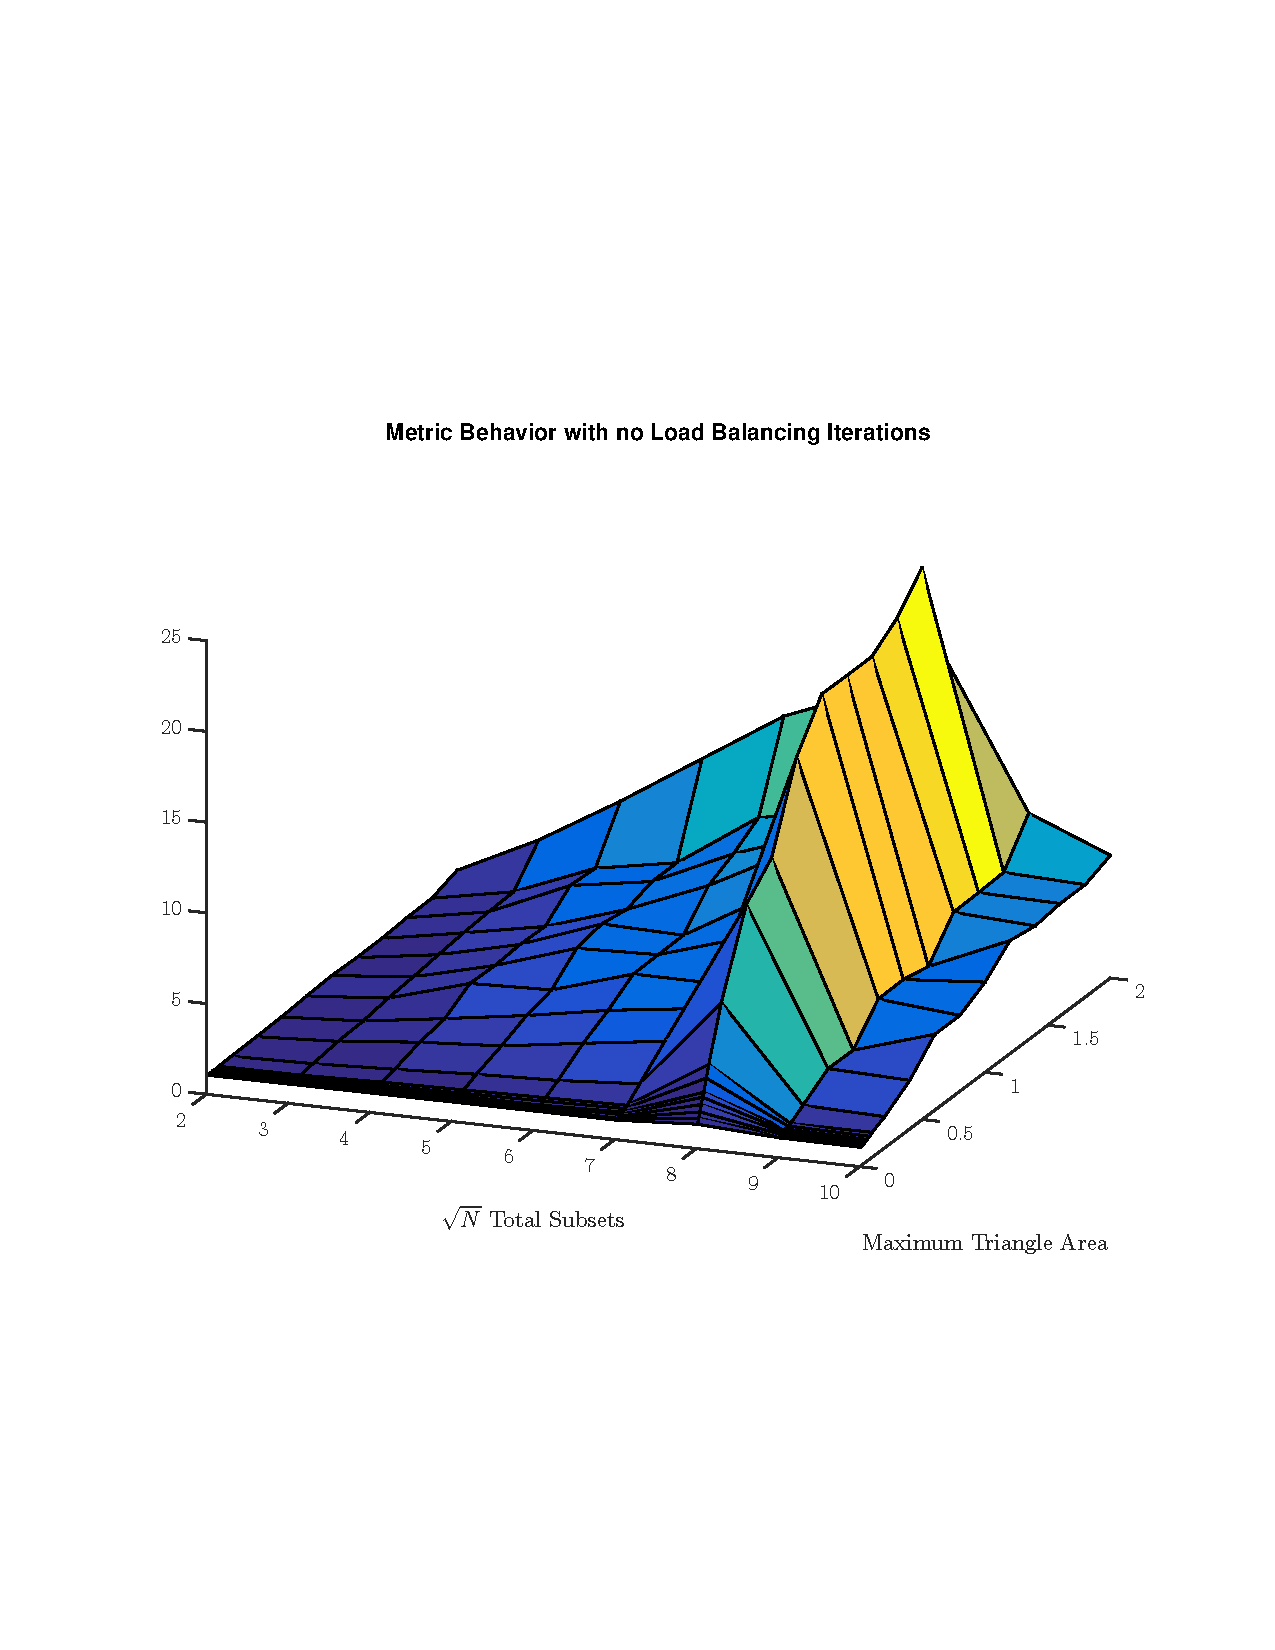
\includegraphics[scale=0.78, trim = 2cm 6cm 2cm 7cm,clip]{figures/SameNoIter.pdf}
\captionof{figure}{The metric behavior of the second test case run with no load balancing iterations.}
\label{samenoiter}
\end{minipage}
\smallskip

Figure \ref{sameiter} shows the metric behavior for Fig. \ref{same} after ten load balancing iterations. The maximum metric is 3.9929 and occurs when Fig. \ref{same} is run with 10x10 subsets with a maximum triangle area of 1.8 cm\textsuperscript{2}. The minimum metric is 1.0024 and occurs when Fig. \ref{same} is run with 2x2 subsets with a maximum triangle are of 0.01 cm\textsuperscript{2}.

\noindent\begin{minipage}{\textwidth}
\centering
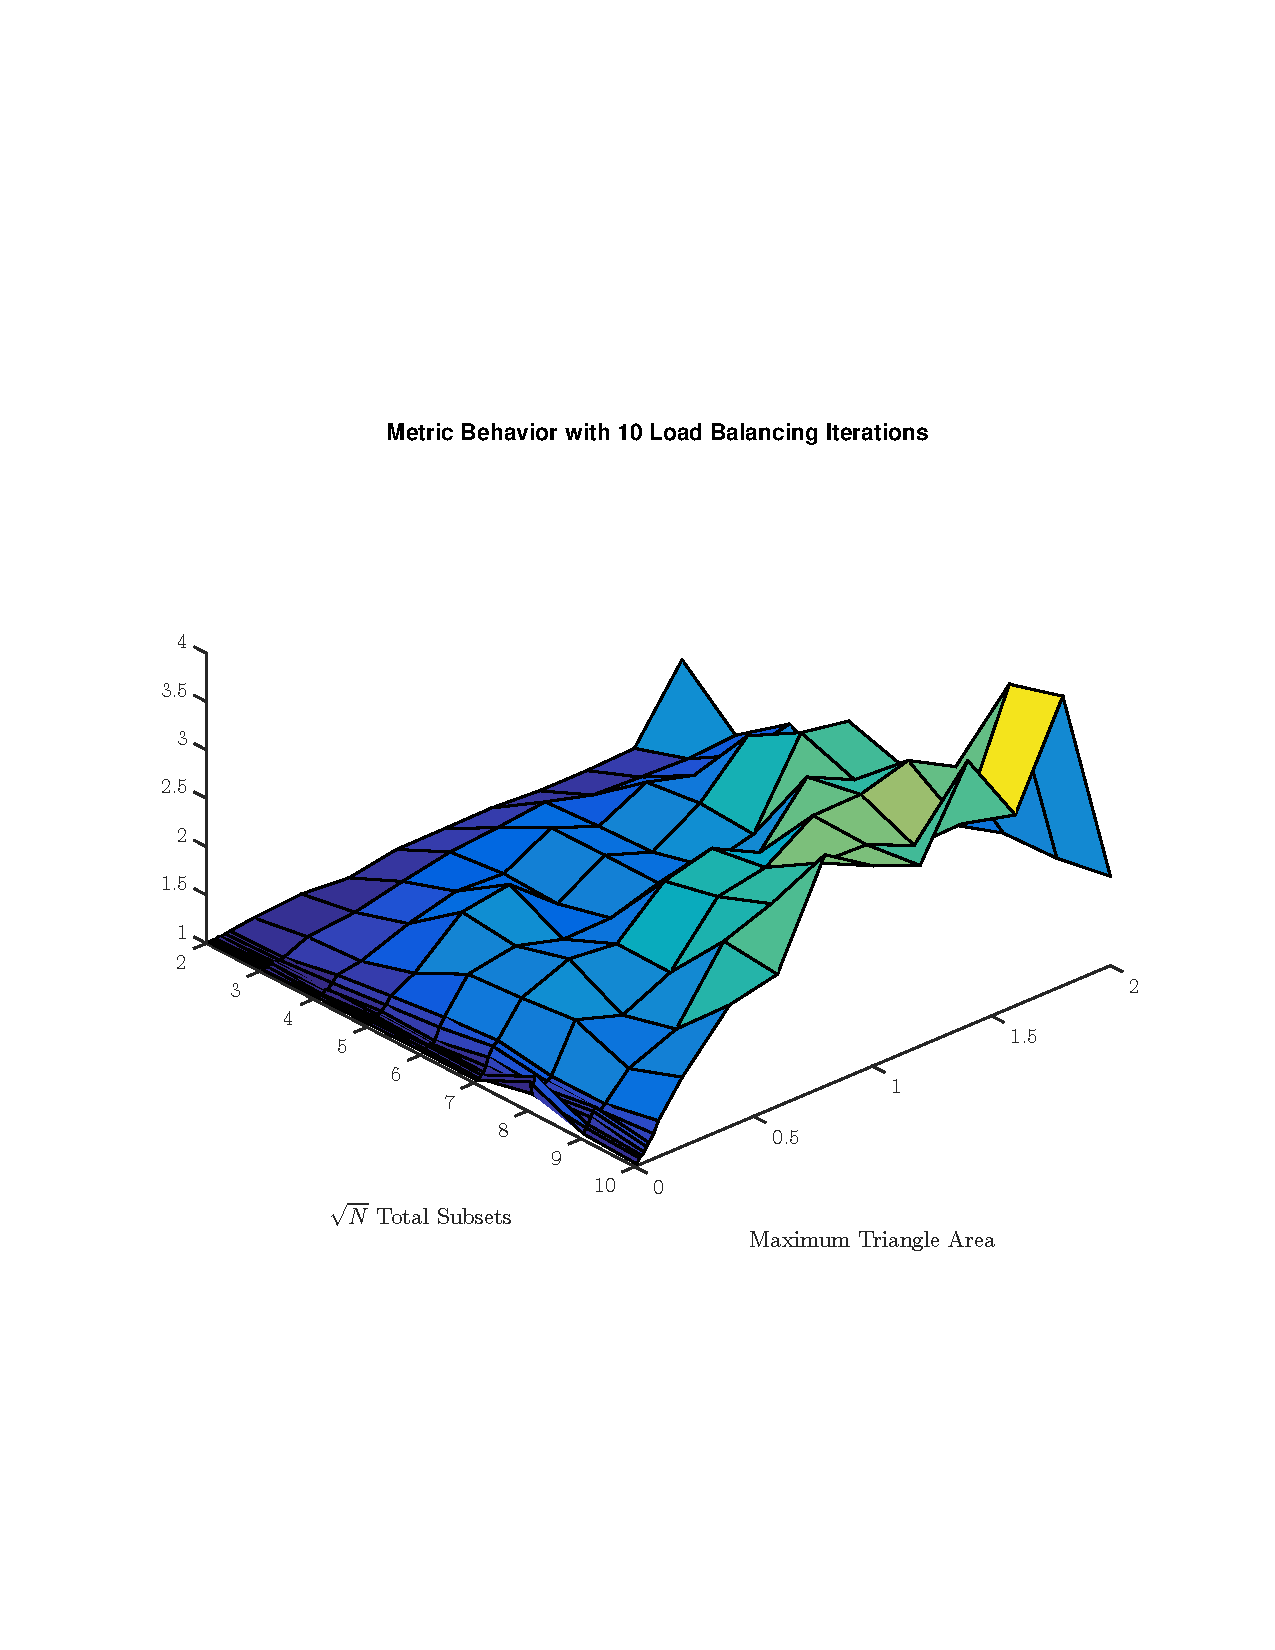
\includegraphics[scale=0.80, trim = 2cm 6cm 2cm 7cm,clip]{figures/SameIter.pdf}
\captionof{figure}{The metric behavior of the second test case run with 10 load balancing iterations.}
\label{sameiter}
\end{minipage}
\smallskip

Figure \ref{samediff} shows the difference in metric behavior for Fig. \ref{same}. The maximum improvement has a value of 0.1090 and occurs for Fig. \ref{same} is run with 8x8 subsets with Triangle's coarsest possible mesh generation settings. The minimum improvement has a value of very close to 1.0 and occurs for many of the inputs. 

\noindent\begin{minipage}{\textwidth}
\centering
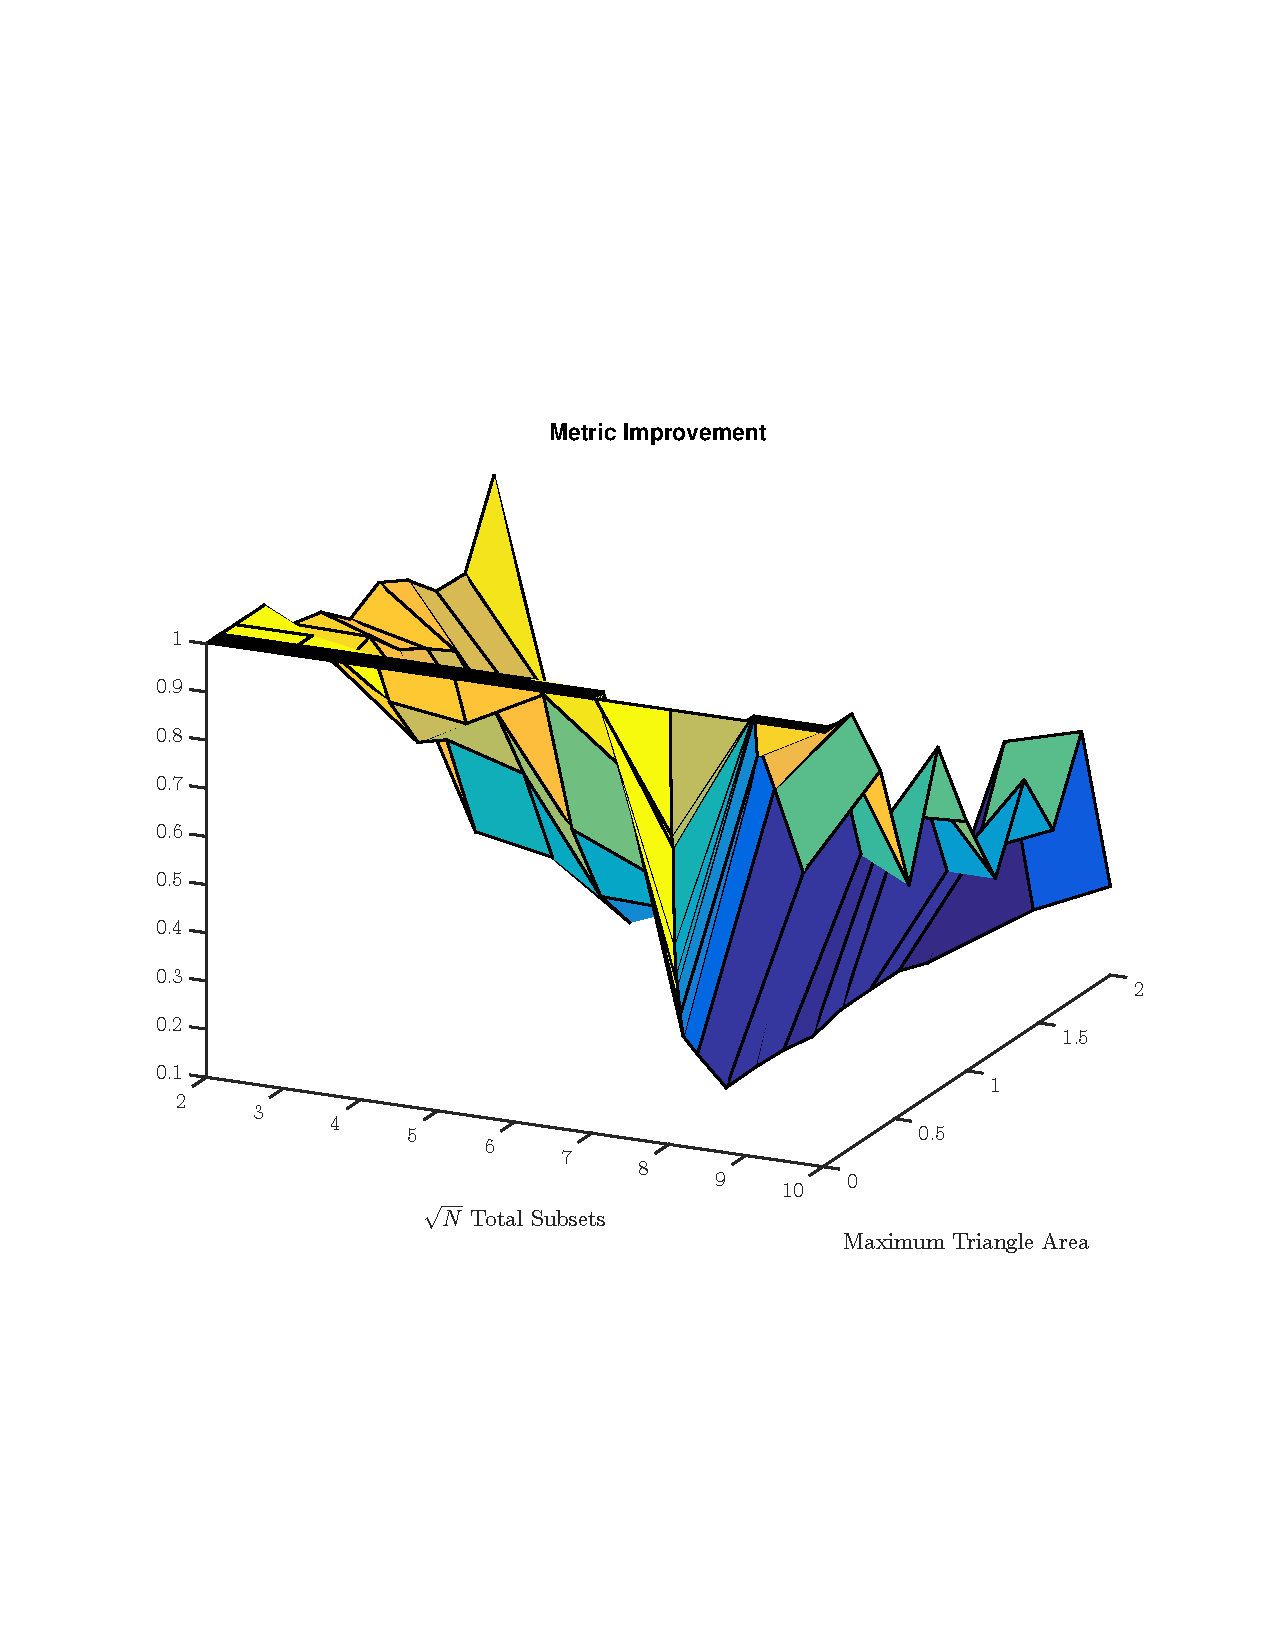
\includegraphics[scale=0.80, trim = 2cm 6cm 2cm 7cm,clip]{figures/SameDiff.pdf}
\captionof{figure}{The difference in metric behavior of the second test case with no iteration and 10 iterations. The closer the z-value to zero, the better the improvement.}
\label{samediff}
\end{minipage}
\smallskip

Figure \ref{latticenoiter} shows the metric behavior for Fig. \ref{lattice}. The maximum metric is 2.6489 and occurs when Fig. \ref{lattice} is run with 10x10 subsets with a maximum triangle area of 1.8 cm\textsuperscript{2}. The minimum metric is 1.0179 and occurs when Fig. \ref{lattice} is run with 2x2 subsets with a maximum triangle are of 0.08 cm\textsuperscript{2}.

\noindent\begin{minipage}{\textwidth}
\centering
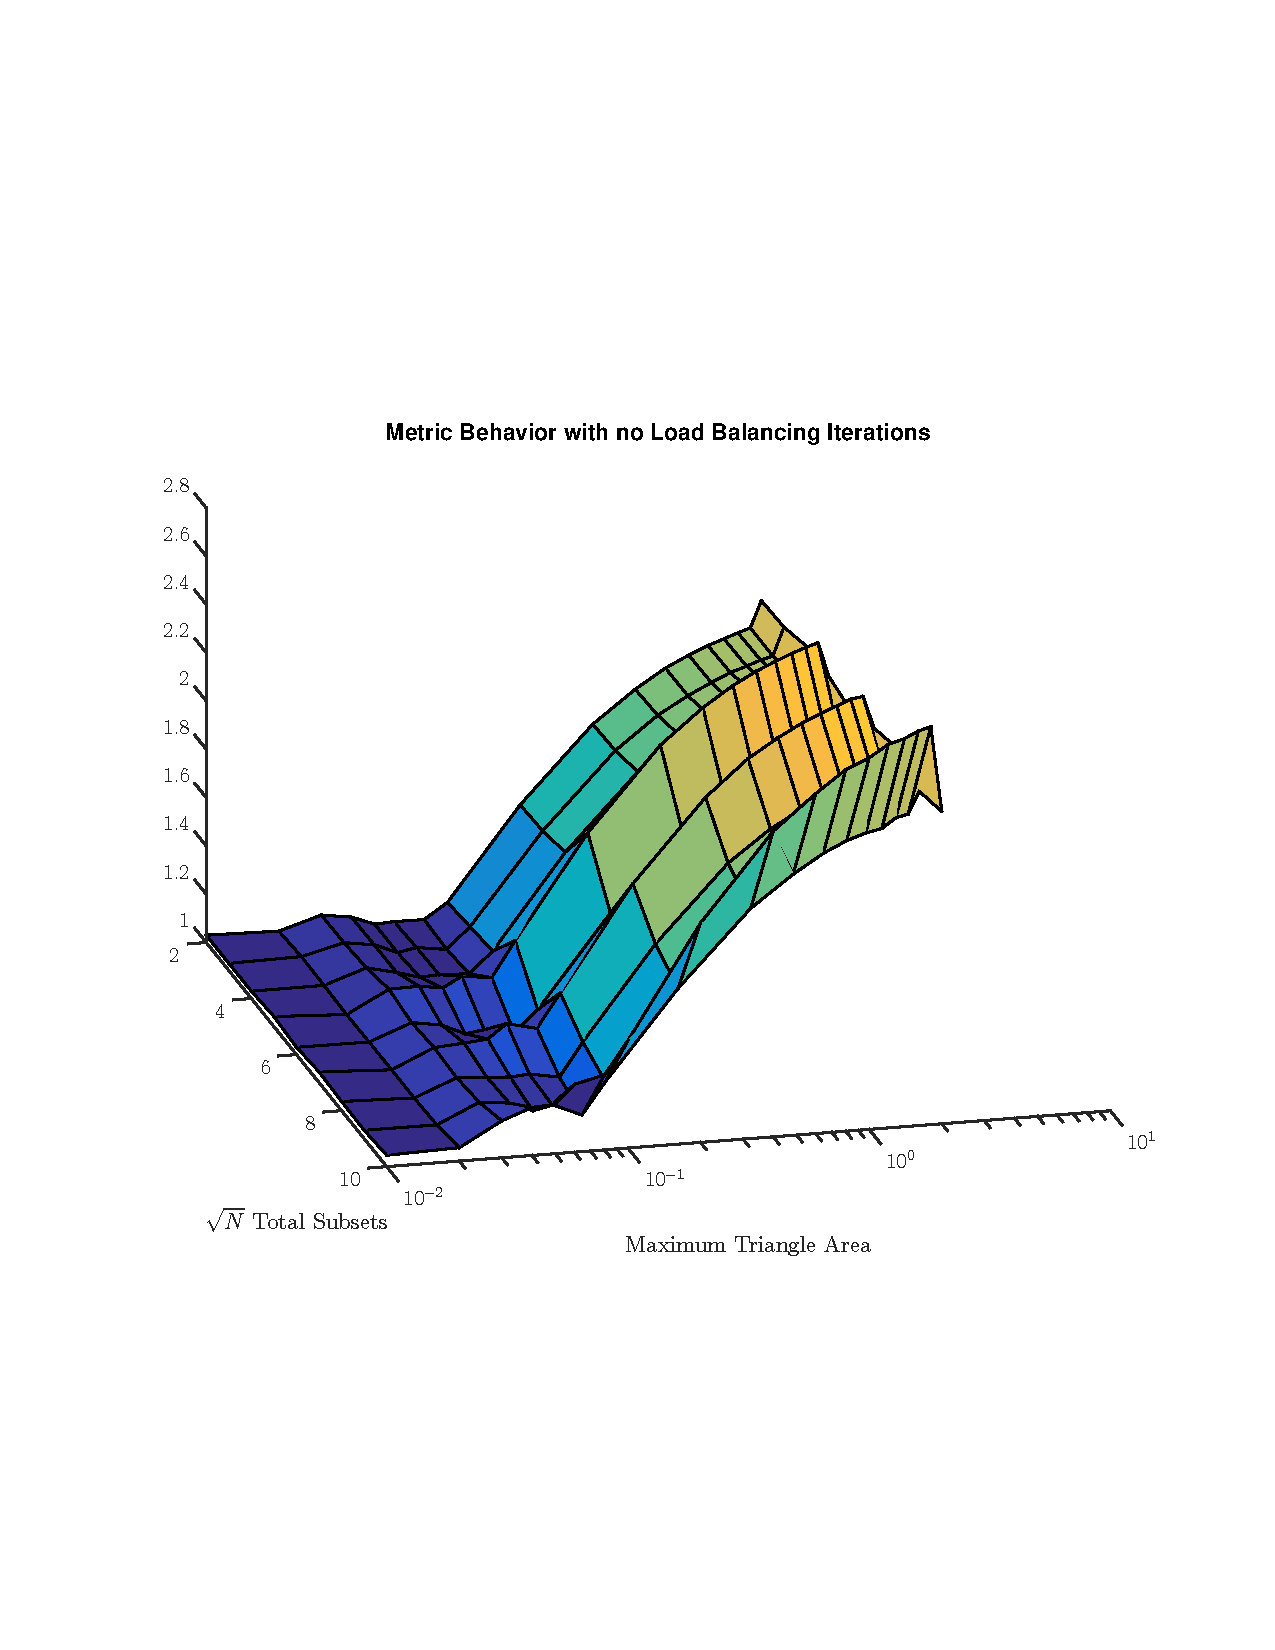
\includegraphics[scale=0.80, trim = 2cm 6cm 2cm 7cm,clip]{figures/lattice_no_iter.pdf}
\captionof{figure}{The difference in metric behavior of the third test case with no load balancing iterations.}
\label{latticenoiter}
\end{minipage}
\smallskip

Figure \ref{latticeiter} shows the metric behavior for Fig. \ref{lattice} after ten load balancing iterations. The maximum metric is 2.2660 and occurs when Fig. \ref{lattice} is run with 10x10 subsets with a maximum triangle area of 0.4 cm\textsuperscript{2}. The minimum metric is 1.0021 and occurs when Fig. \ref{lattice} is run with 2x2 subsets with the Triangle's coarsest possible mesh.

\noindent\begin{minipage}{\textwidth}
\centering
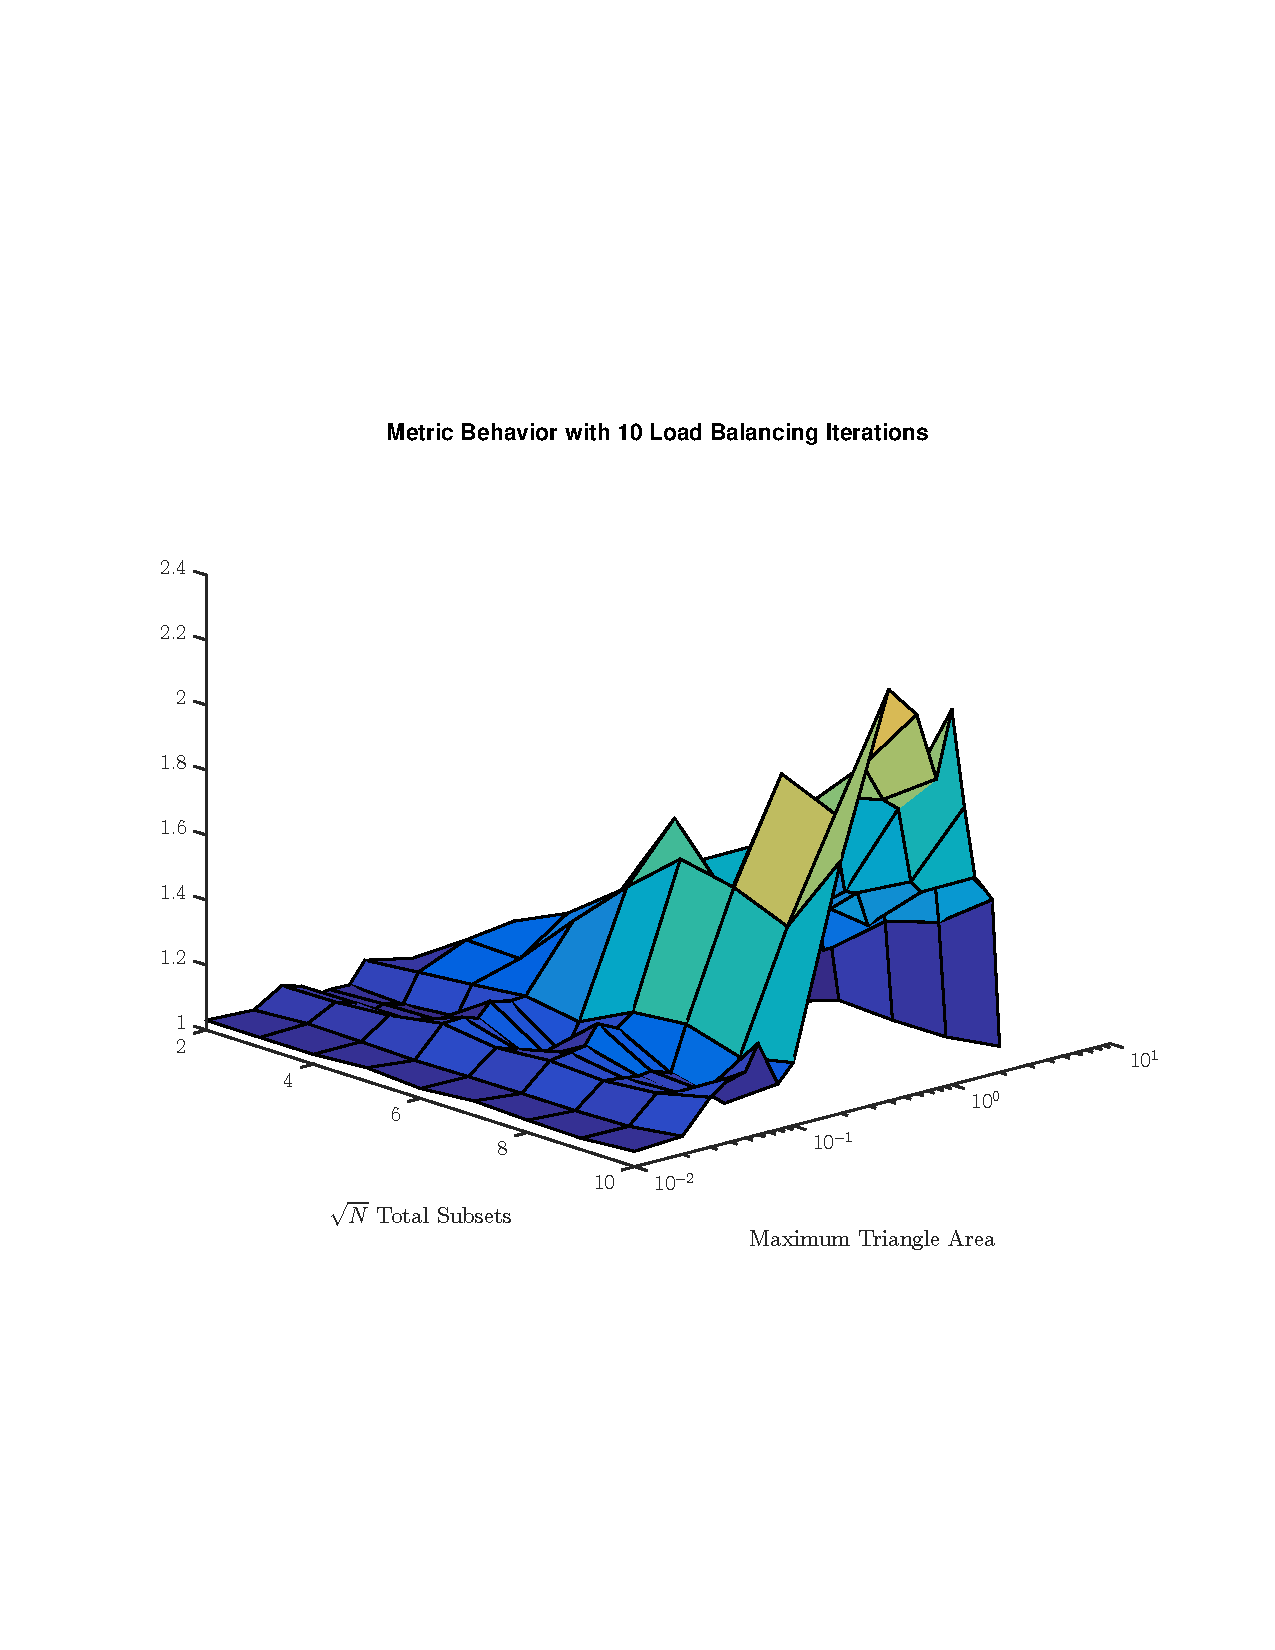
\includegraphics[scale=0.80, trim = 2cm 6cm 2cm 7cm,clip]{figures/lattice_iter.pdf}
\captionof{figure}{The difference in metric behavior of the third test case after ten load balancing iterations.}
\label{latticeiter}
\end{minipage}
\smallskip

Figure \ref{latticediff} shows the difference in metric behavior for Fig. \ref{lattice}. The maximum improvement has a value of 0.4476 and occurs for Fig. \ref{lattice} is run with 2x2 subsets with Triangle's coarsest possible mesh generation settings. The minimum improvement has a value of very close to 1.0 and occurs for many of the inputs. 

\noindent\begin{minipage}{\textwidth}
\centering
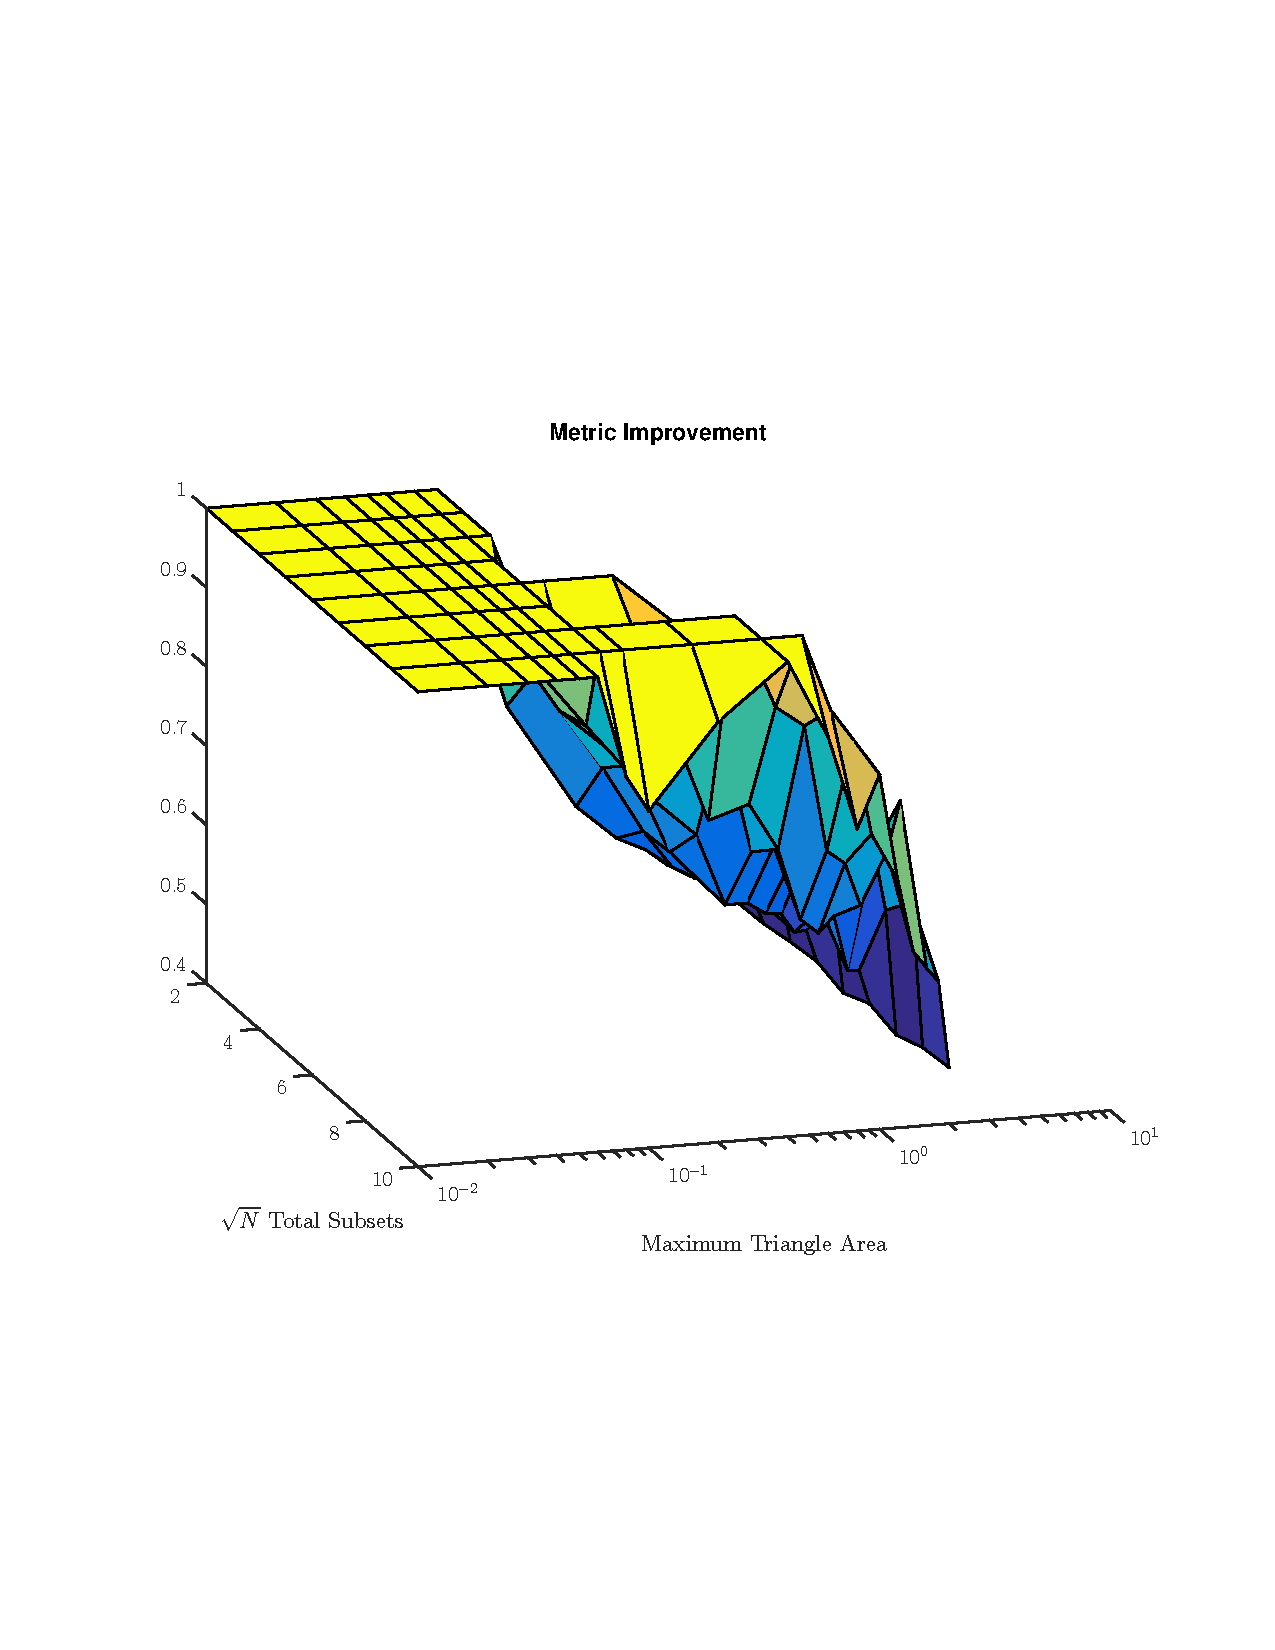
\includegraphics[scale=0.80, trim = 2cm 6cm 2cm 7cm,clip]{figures/lattice_diff.pdf}
\captionof{figure}{The difference in metric behavior of the third test case with no iteration and 10 iterations. The closer the z-value to zero, the better the improvement.}
\label{latticediff}
\end{minipage}
\smallskip

Because Fig. \ref{lattice} has more features and is more symmetric of a problem, the initial load balancing metric will not be as large as the load balancing metric of Figs. \ref{same} and \ref{opp}. As a result, the improvement in the load balancing metric after 10 iterations will not be as great in problems similar to Fig. \ref{lattice}. 

Good improvement is seen throughout all three test cases for all three inputs, particularly the first two test cases, which were initially very unbalanced. However, there were many inputs run that had problems with $f > 1.1$, which means many problems were unbalanced by more than 10\%. The user will not always have the luxury of choosing the number of subsets they want the problem run with, as this directly affects the number of processors the problem will be run with. Certain problems will require more processors and will require minimizing the total number of cells in the domain for the problem to complete running in a reasonable amount of time. As a result, improvements to the algorithm must be made. 

This can be done by changing how the cut lines are redistributed. Instead of changing entire row and column widths, the cut lines can be moved on the subset level. However, this can sacrifice the strict orthogonality that PDT currently utilizes to scale so well on a massively parallel scale. Changes to the performance model and the scheduler would have to be made.

Another option is to implement domain overloading, which is the logical extension of the work presented in this thesis. This would involve processors owning different numbers of subsets, with no restriction on these subsets being contiguous. This would be the most effective method at perfecting this algorithm, and would lead to less problems being unbalanced by more than 10\%.

\section{Solution Verification}

For solution verification, two simple problems were chosen: a 1D pure absorber slab and a 1D pure scatterer slab. These problems were chosen because their analytical solutions are easily obtained, thus making a comparison between PDT's solution and the analytical solution easy and informative. The same geometry and mesh were used for both problems, and are shown in Figure \ref{verificationgeometry}.

\noindent\begin{minipage}{\textwidth}
\centering
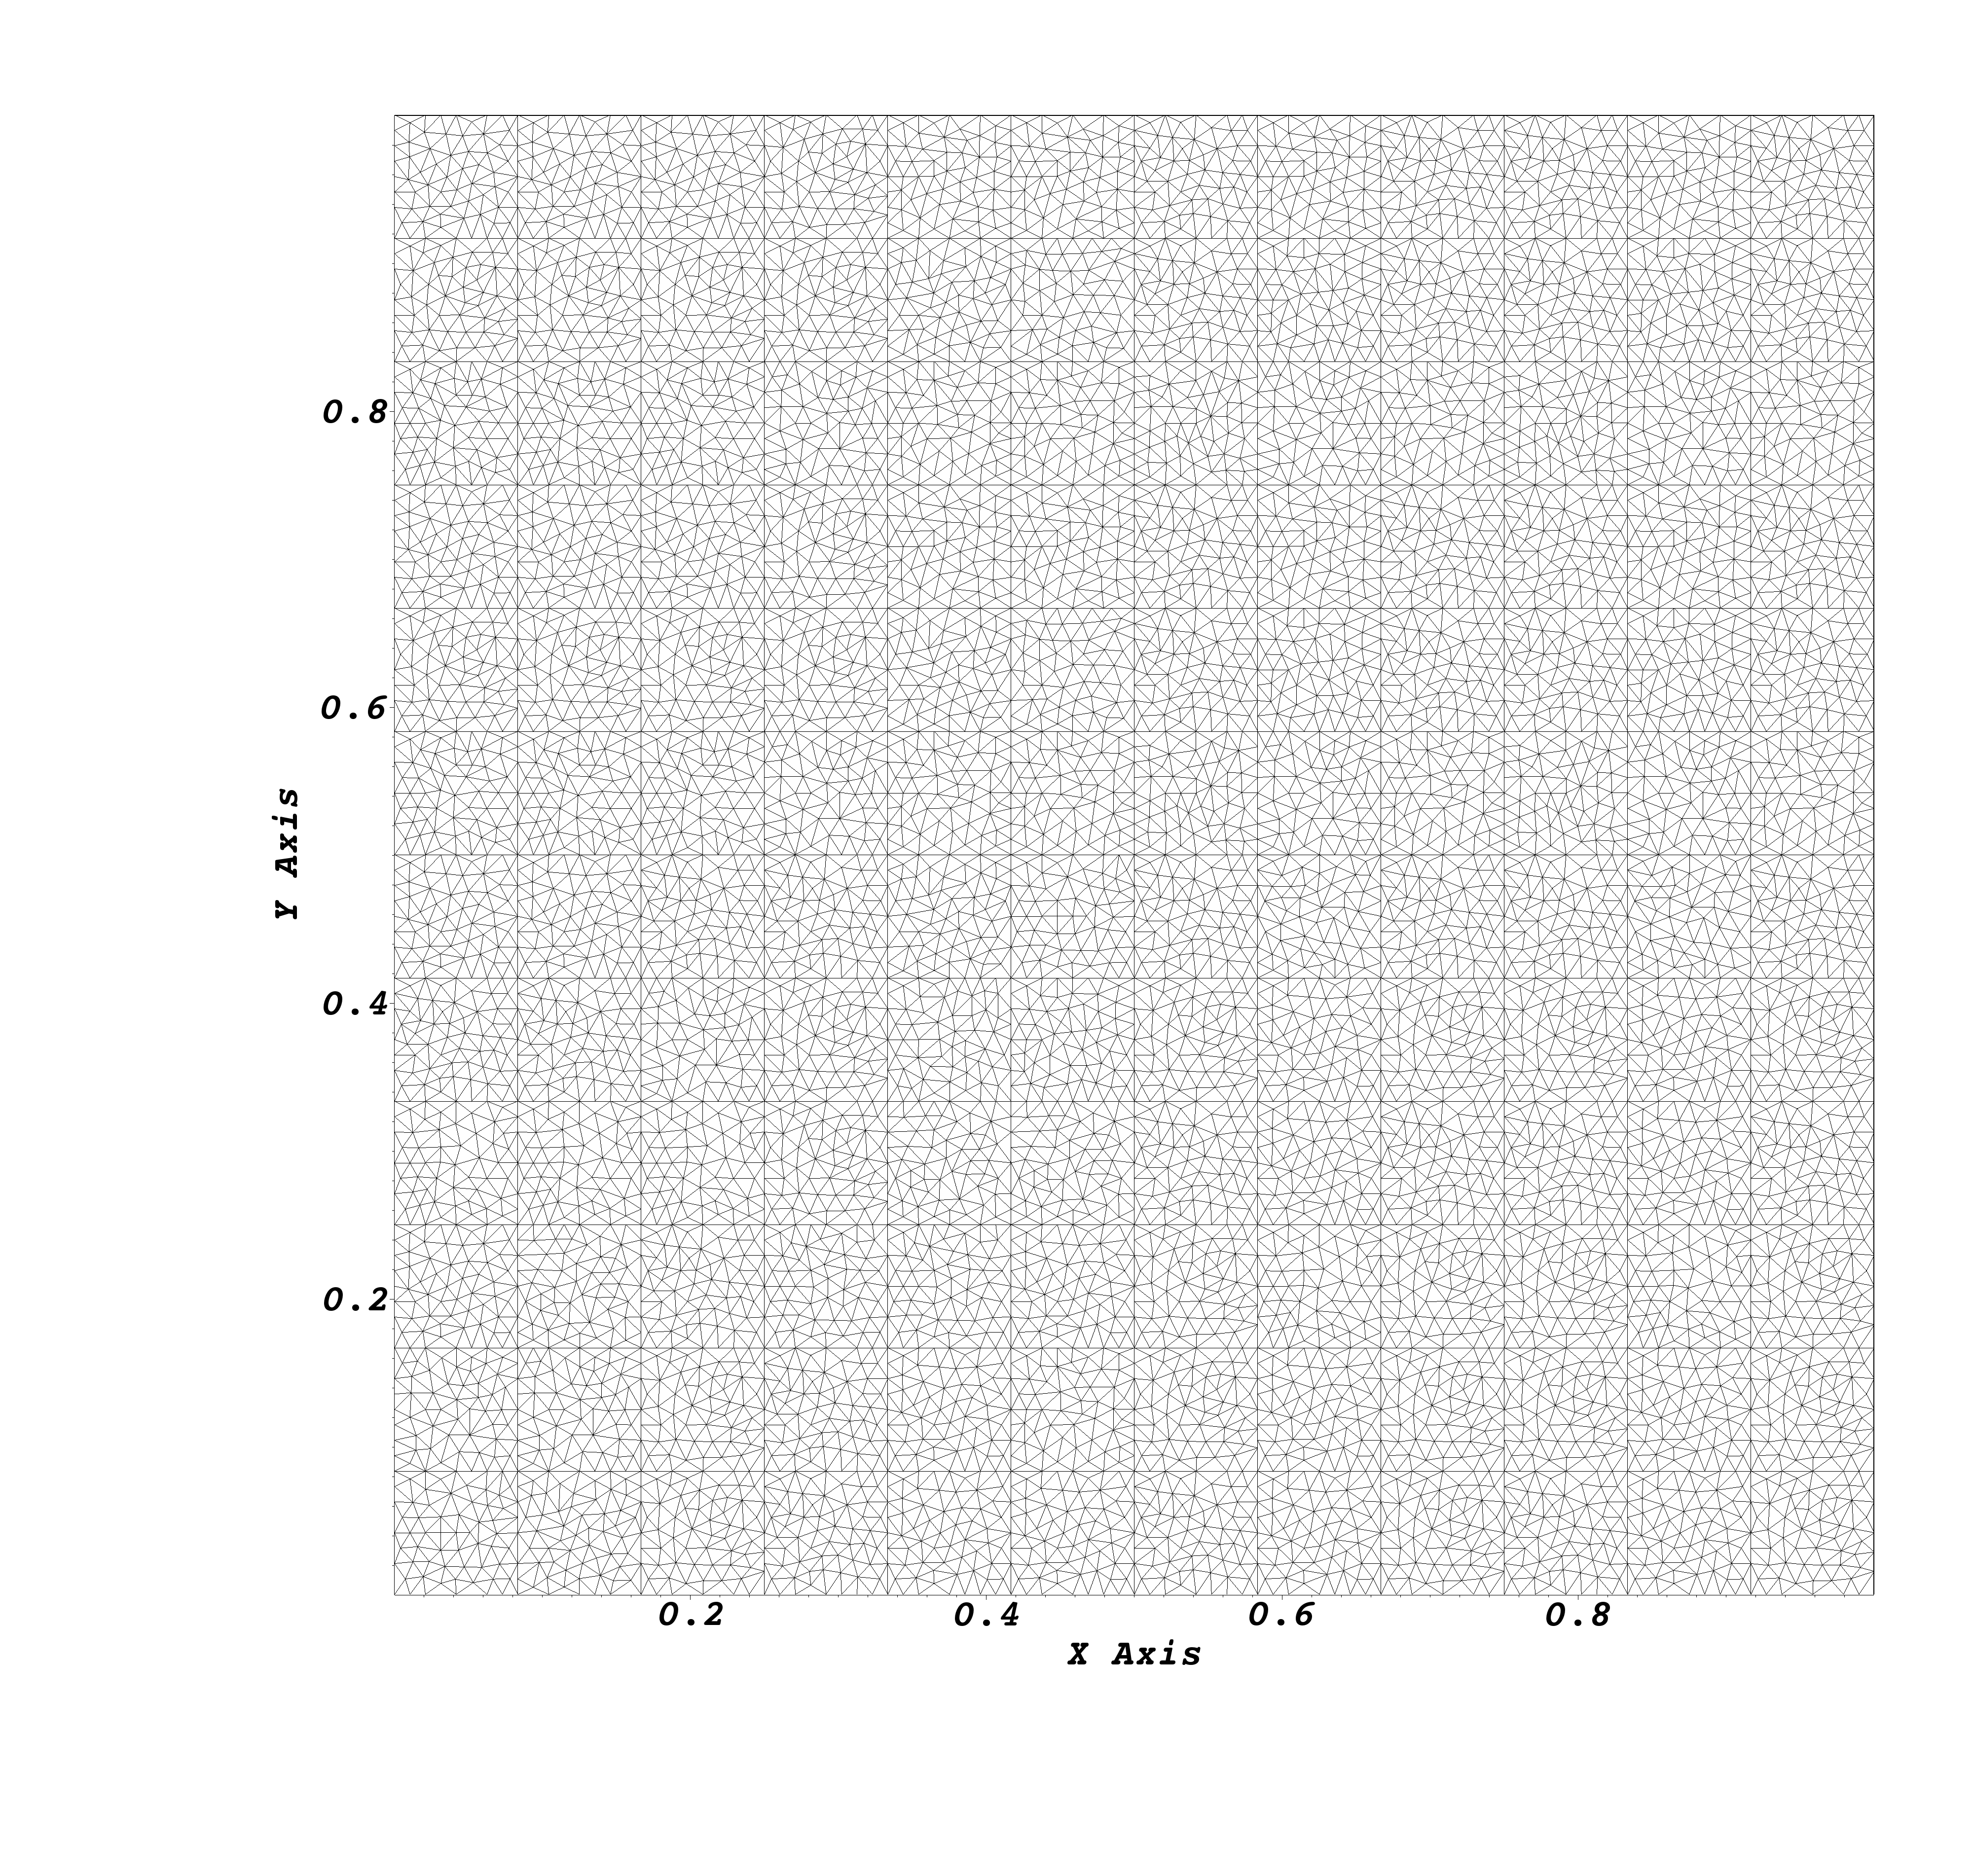
\includegraphics[scale = 0.12,trim = 10cm 10cm 0cm 0cm ]{figures/solutionmesh.png}
\captionof{figure}{The geometry and mesh used in solution verification problems.}
\label{verificationgeometry}
\end{minipage}
\smallskip

The problem geometry is a 1 cm by 1 cm square. In order to simulate a 1D slab, opposing reflecting boundaries were placed on the both y boundaries, effectively forcing the problem to be infinite in the y direction. At the x minimum boundary, an incident isotropic flux was used, and a vacuum boundary was enforced at the x max boundary. No source was used in either problem.

In order to measure how close the numerical and analytical solutions an error estimate, represented by, Eq. ~\eqref{error}, is used:
\begin{equation}
\epsilon = \frac{\norm{\text{Analytical} - \text{ Numerical}}_{l2}}{\norm{\text{Analytical}}_{l2}},
\label{error}
\end{equation}
where the $l2$ norm of the absolute error is divided by the $l2$ norm of the analytical solution.

\subsection{The 1D Pure Absorber Slab}

For monoenergetic neutrons, a source free, 1D pure absorber slab, the transport equation is represented by Eq. ~\eqref{absorbertransport}:
%Absorber transport
\begin{equation}
\mu \frac{d\psi (x,\mu>0)}{dx} + \Sigma_a \psi(x,\mu>0) = 0,
\label{absorbertransport}
\end{equation}
where $\psi$ is the angular flux, $\Sigma_a$ is the macroscopic absorption cross section, and $\mu$ is the cosine of the polar angle. The boundary conditions for this problem are expressed in Eq. ~\eqref{boundaryconditions}:
\begin{align}
\label{boundaryconditions}
\psi(0,\mu>0) &= \int_{0}^{2\pi}d\gamma \int_{0}^{1}\frac{\psi_{0}}{4\pi} d\mu = \frac{\psi_{0}}{2}  = \psi_{inc} \text{ (incident isotropic)} \notag \\
\psi(x_{\text{max}},\mu<0) &= 0 \text{ (vacuum)},
\end{align}
where $\psi_{0}$ is the user defined value of the incident isotropic angular flux, and $\psi_{inc}$ is the angular flux at $x = 0$. Equation ~\eqref{absorber_derivation} solves the transport equation via separation of variables to get the angular flux for this problem:
%absorber derivation
\begin{align}
\label{absorber_derivation}
\frac{d\psi(x,\mu>0)}{dx} &= -\frac{\Sigma_a}{\mu} x \notag \\
\frac{d\psi(x,\mu>0)}{\psi(x,\mu>0)} &= -\frac{\Sigma_a}{\mu} x dx \notag \\
\int_{\psi(0,\mu>0)}^{\psi(x,\mu>0)}\frac{d\psi(x,\mu>0)}{\psi(x,\mu>0)} &= \int_{0}^{x}-\frac{\Sigma_a}{\mu} x' dx' \notag \\
\ln[\frac{\psi(x,\mu>0)}{\psi(0,\mu>0)}] &= -\frac{\Sigma_a}{\mu} x \notag \\
\psi(x,\mu>0) & = \psi(0,\mu>0)\exp(-\frac{\Sigma_a}{\mu} x) \notag \\
\psi(x,\mu>0) & = \psi_{inc}\exp(-\frac{\Sigma_a}{\mu} x) 
\end{align}

Using the fact that the scalar flux in this pure absorber is simply the angular flux integrated for $\mu > 0$, the scalar flux with our boundary conditions is represented by Eq. ~\eqref{absorberflux}:
%Absorber flux
\begin{align}
\phi(x) &= \int_{0}^{1}\psi(x,\mu>0) d\mu \notag \\
&= \int_{0}^{1}\psi_{inc}\exp(-\frac{\Sigma_a}{\mu} x) d\mu = \psi_{inc} E_{2}(\Sigma_a x),
\label{absorberflux}
\end{align}
where $\phi$ is the scalar flux and $E_2$ is the exponential integral function with $n=2$. 

The pure absorber was run with $\psi_{inc} = 3.5 \frac{\text{n}}{\text{cm}^2\text{-s-ster}}$ and $\Sigma_a = 5 \text{ cm}^{-1}$. Figure \ref{pa_allangles} shows a comparison of the analytical solution with PDT's solution for four different angular refinements. All four PDT runs used only 1 azimuthal angle per quadrant, but varied the number of positive polar angles, because the problem is not azimuthally dependent. The number of positive polar angles used were 1,5,10, and 70. 

\noindent\begin{minipage}{\textwidth}
\centering
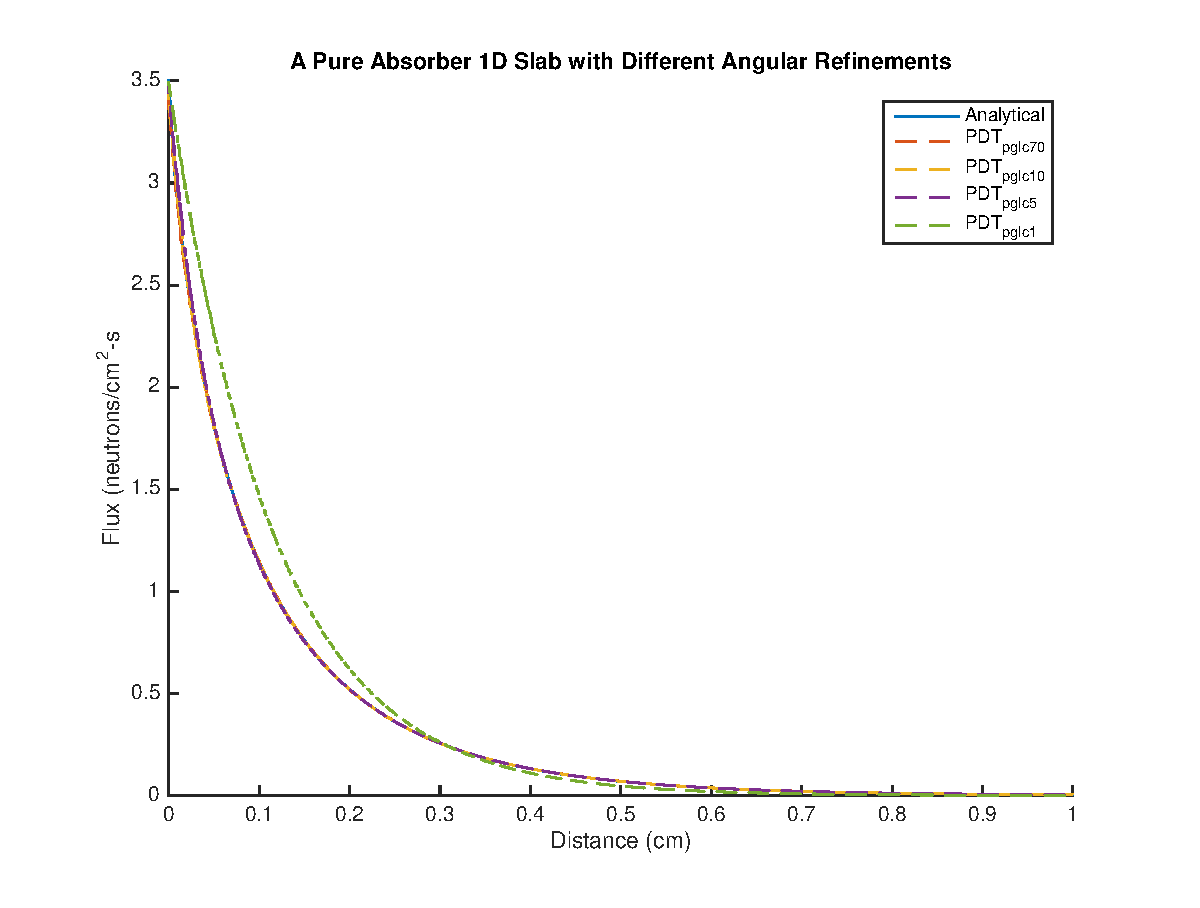
\includegraphics[scale = 0.8]{figures/PureAbsorberAllAngles.eps}
\captionof{figure}{The pure absorber solution with four different angular refinements.}
\label{pa_allangles}
\end{minipage}
\smallskip

It is immediately clear that not many polar angles are necessary for agreement with the analytical solution. Figure \ref{pa_bestangle} examines the 70 positive polar angle case exclusively in comparison with the analytical solution. It is immediately clear graphically that the solutions are in agreement, and the relative error of the numerical solution is 0.012, as defined by Eq. ~\eqref{error}.

\noindent\begin{minipage}{\textwidth}
\centering
\includegraphics[scale = 0.8]{figures/PureAbsorberBestangle.eps}
\captionof{figure}{The pure absorber solution run with 70 positive polar angles.}
\label{pa_bestangle}
\end{minipage}
\smallskip

\subsection{The 1D Pure Scatterer Slab}

For an optically thick, source free 1D pure absorber with monoenergetic neutrons, the transport solution will reach the diffusion limit. The diffusion equation for this problem is represented by Eq. ~\eqref{diffusion}:
%Scattering equation
\begin{equation}
\frac{d^2\phi}{dx^2} = 0,
\label{diffusion}
\end{equation}
where $\phi$ is the scalar flux. The boundary conditions for this problem are expressed in Eq. ~\eqref{scatterboundary}:
%Scatter bc's
\begin{align}
\phi(-2D) &= 4j_{inc} \notag \\
\phi(x_{\text{max}}+2D) &= 0, 
\label{scatterboundary}
\end{align}
where $j_{inc}$ is the incident partial current and $D$ is the diffusion coefficient, which is equivalent to $\frac{1}{3 \Sigma_t}$, where $\Sigma_t$ is the total macroscopic cross section. The first boundary condition is the extrapolated boundary condition, and the second is the extrapolated vacuum condition. The incident partial current is calculated from the incident angular flux, as shown in Eq. ~\eqref{partialcurrent}:
%Partial current
\begin{equation}
j_{inc} = \int_{0}^{2\pi}d\gamma \int_{0}^{1} \mu \frac{\psi_{inc}}{4\pi} d\mu = \frac{\psi_{inc}}{4}.
\label{partialcurrent}
\end{equation}

The integral over polar angles in Eq. ~\eqref{partialcurrent} is the result of computing the angular quadrature with an infinite number of polar angles. Table \ref{angleconvergence} shows the value of $j_{inc}$ converging to the integral value as the number of polar angles is increased. 
\begin{table}[H]
\centering
\caption{The convergence of $j_{inc}$ as the number of polar angles increase.}
\begin{tabular}{c c}
\hline
\textbf{Number of Positive Polar Angles} & \textbf{$j_{inc}$} \\
1 & 2.0207 \\
2 & 1.8244 \\
5 & 1.7632 \\
10 & 1.7534 \\
20 & 1.7509 \\
40 & 1.7502 \\
Infinite & 1.750 \\
\hline
\end{tabular}
\label{angleconvergence}
\end{table}

Equation ~\eqref{scalarflux} solves Eq. ~\eqref{diffusion}:
\begin{align}
\frac{d\phi(x)}{dx} &= A \notag \\
\phi(x) &= Ax + B,
\label{scalarflux}
\end{align}
where A and B are integration constants. Using our boundary conditions in Eq ~\eqref{scatterboundary} to solve for A and B:
\begin{align}
\phi(-2D) &= -2DA + B = 4j_{inc} \notag \\
\phi(x_{\text{max}} + 2D) &= A(x_{\text{max}} + 2D) + B = 0, \notag
\label{notimportant}
\end{align}
the scalar flux, represented by Eq. ~\eqref{scatterflux}, is:
%Scatter flux
\begin{equation}
\phi(x) = \frac{4j_{inc}}{1+4D}(-x + x_{\text{max}} + 2D).
\label{scatterflux}
\end{equation}

This problem was run with $\Sigma_t = 100 \text{ cm}^{-1}$ and $j_{inc} = \frac{7}{4} \frac{\text{n}}{\text{cm}^2\text{-s}}$. Figure \ref{scattersoln} shows the agreement between the analytical solution and PDT's solution. An angular refinement of 40 polar angles was used, with one azimuthal angle in each quadrant.

\noindent\begin{minipage}{\textwidth}
\centering
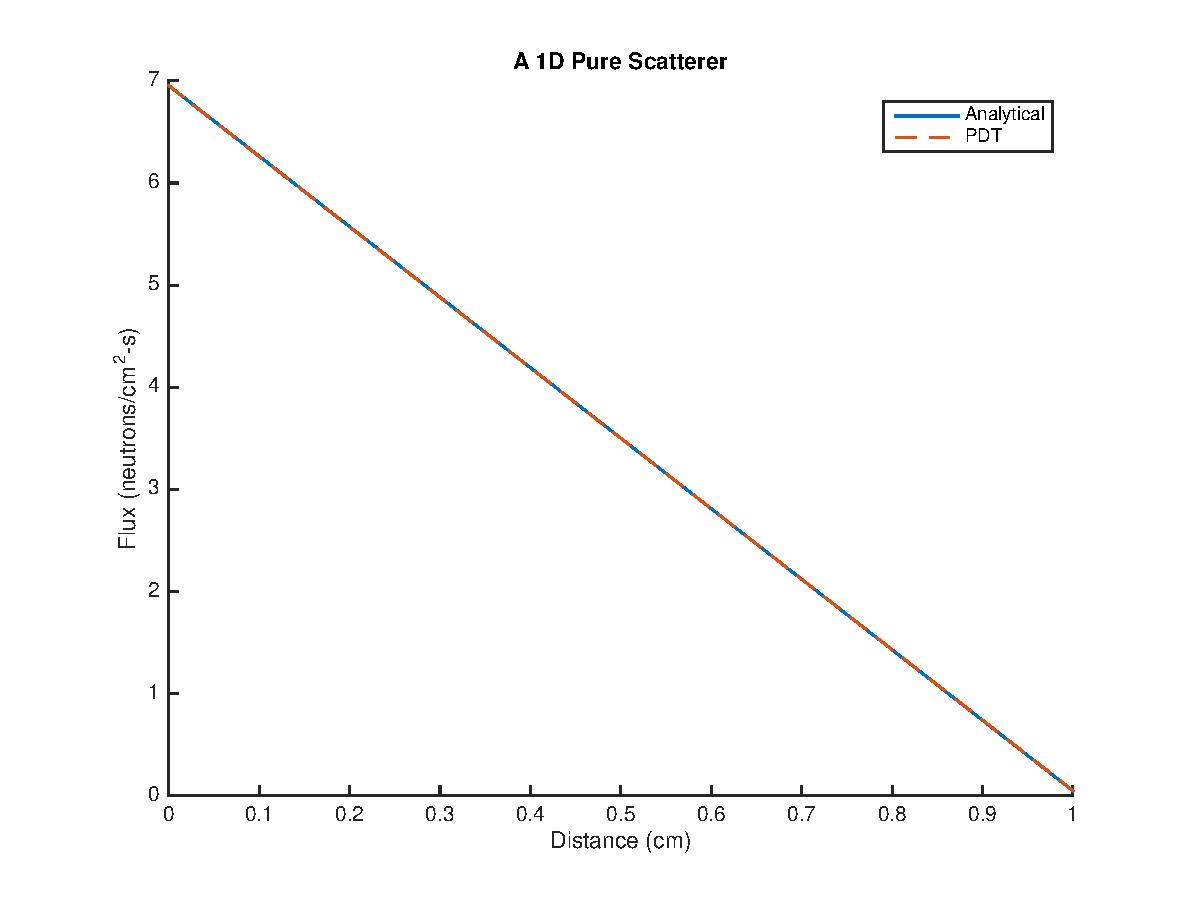
\includegraphics[scale = 0.8]{figures/PureScatterer.eps}
\captionof{figure}{The pure scatterer solution run with 40 positive polar angles.}
\label{scattersoln}
\end{minipage}
\smallskip

It is immediately clear graphically that the two solutions are in agreement, and the relative error of the numerical solution is 4.25E-04, as defined by Eq. ~\eqref{error}.

\section{2D and 2D Extruded Meshing Capability}

To showcase, the newly implemented unstructured meshing capability in PDT, Texas A\&M Nuclear Engineering's Impurity Model 1 (IM1) problem is used. Figure \ref{IM12D} showcases the 2D mesh of the IM1 problem,

\noindent\begin{minipage}{\textwidth}
\centering
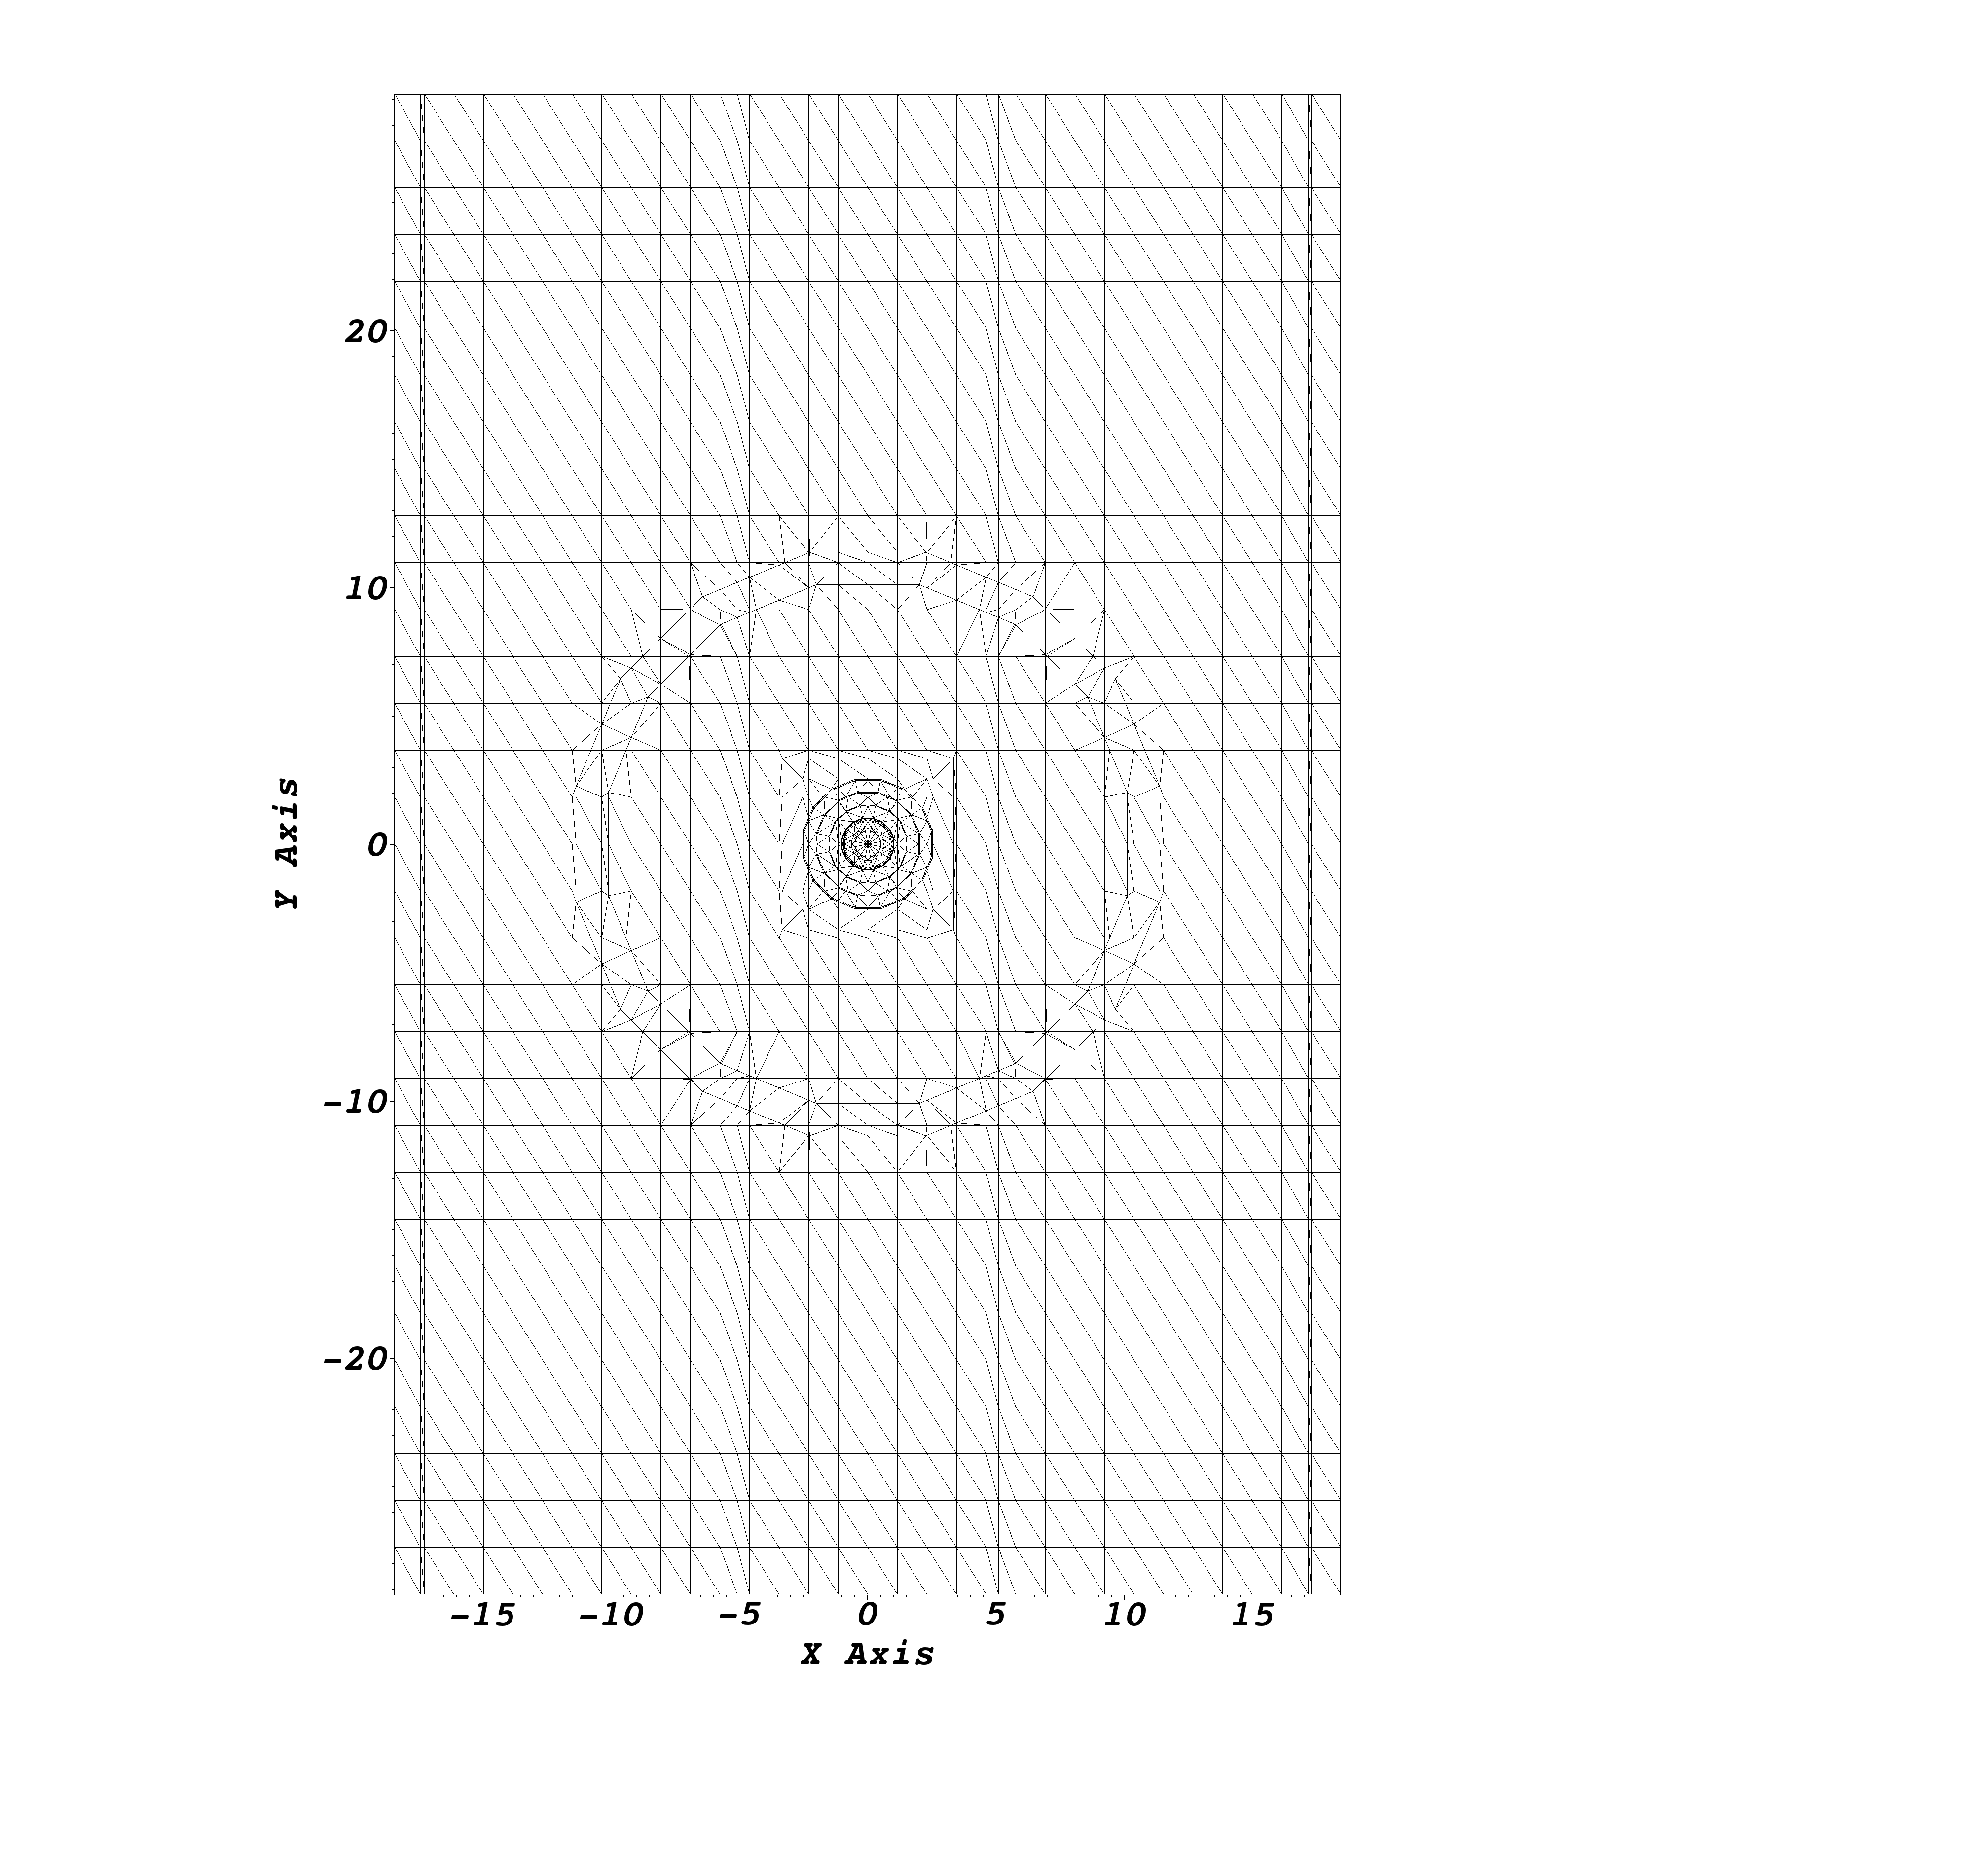
\includegraphics[scale = 0.13]{figures/im12d.png}
\captionof{figure}{The 2D mesh of the IM1 problem.}
\label{IM12D}
\end{minipage}
\smallskip

In order to get from the 2D mesh to the 2D extruded mesh, an extrusion file is supplied to PDT. This extrusion file supplies two critical pieces of information: the number of z layers and their locations, and how each region of the 2D mesh is mapped to these z layers. The combination of the 2D mesh and the extrusion file yield the full 3D problem, shown in Fig. \ref{IM13D}.

\noindent\begin{minipage}{\textwidth}
\centering
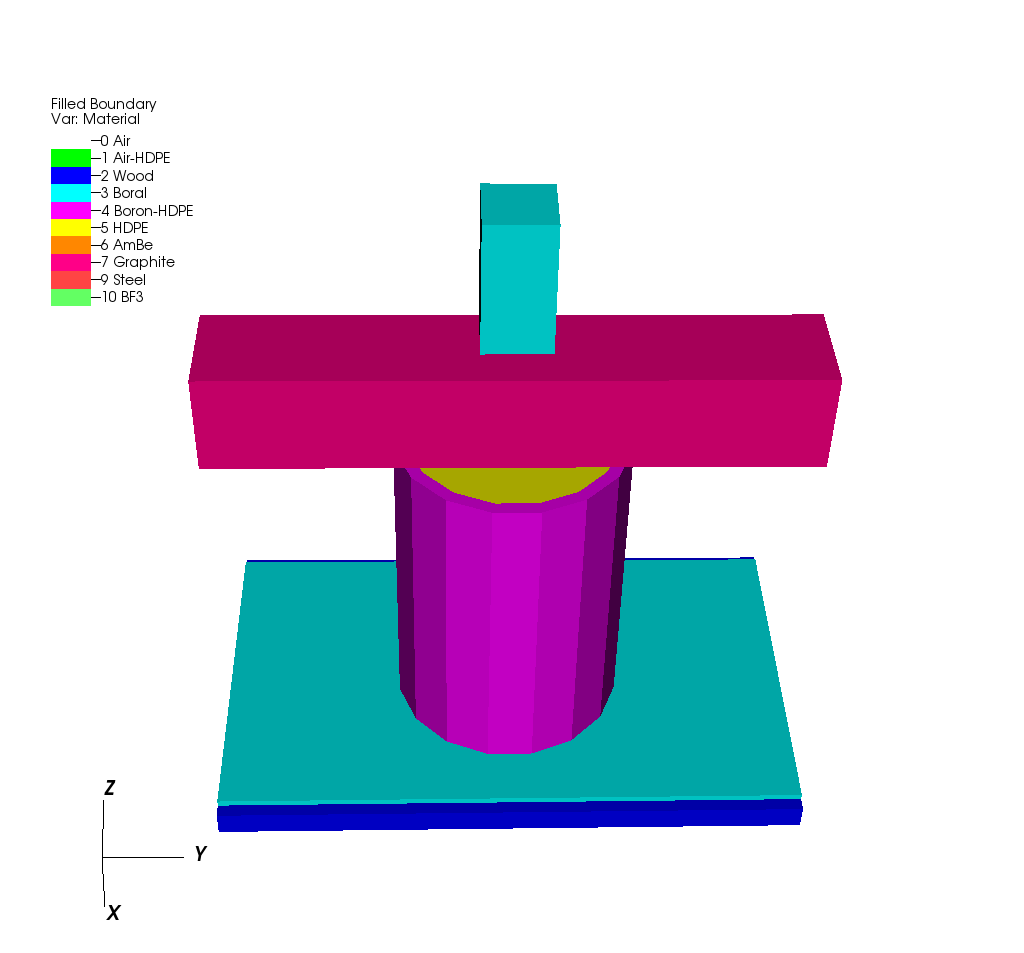
\includegraphics[scale = 0.5]{figures/IM1_3D.png}
\captionof{figure}{The 2D extruded view of the IM1 problem.}
\label{IM13D}
\end{minipage}
\smallskip

%\noindent\begin{minipage}{\textwidth}
%\centering
%\hspace*{-3 cm}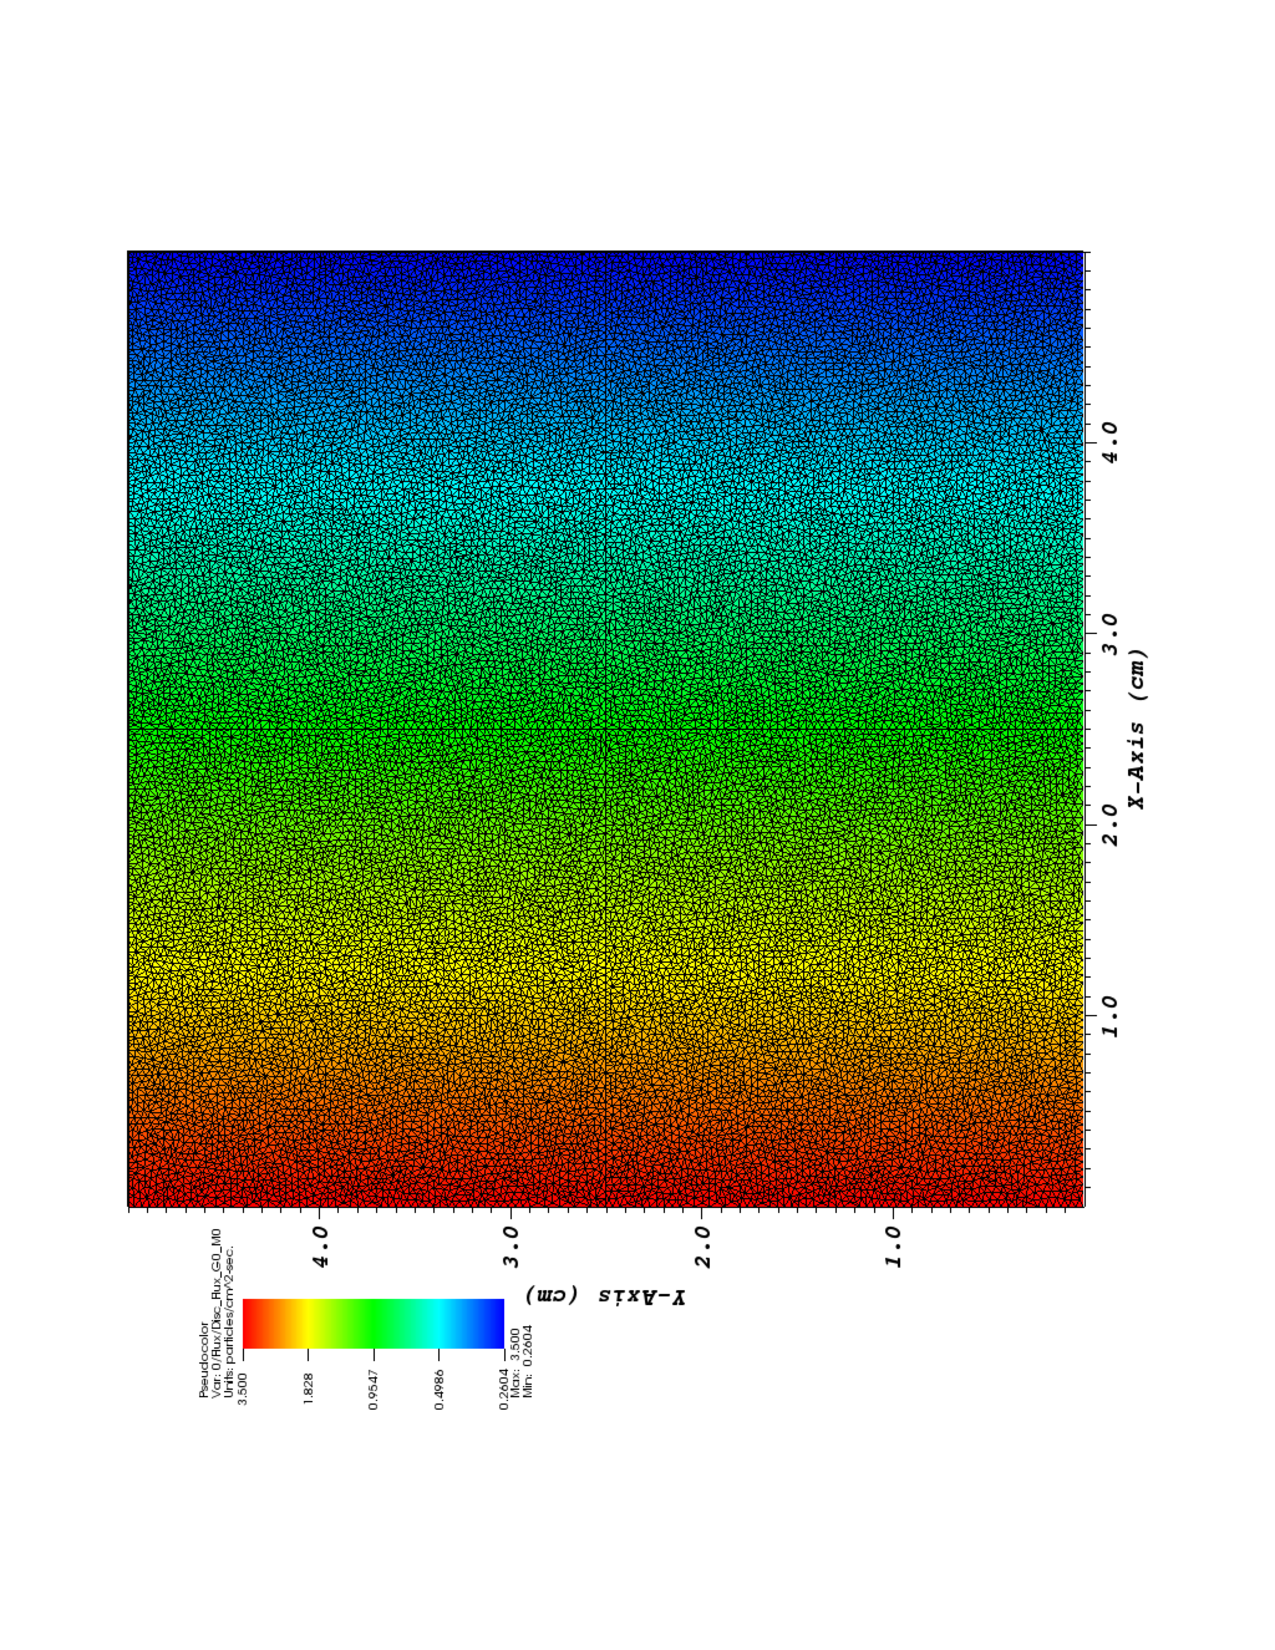
\includegraphics[scale=0.8,angle=-90]{figures/PureAbsorberSolution.pdf}
%\captionof{figure}{The solution of a pure absorbing slab.}
%\label{pureabsorber}
%\end{minipage}

%%%%%%%%%%%%%%%%%%%%%%%%%%%%%%%%%%%%%%%%%%%%%%%%%%%
%
%  New template code for TAMU Theses and Dissertations starting Fall 2016.
%
%
%  Author: Sean Zachary Roberson
%  Version 3.17.09
%  Last Updated: 9/21/2017
%
%%%%%%%%%%%%%%%%%%%%%%%%%%%%%%%%%%%%%%%%%%%%%%%%%%%
%%%%%%%%%%%%%%%%%%%%%%%%%%%%%%%%%%%%%%%%%%%%%%%%%%%%%%%%%%%%%%%%%%%%%%
%%                           SECTION IV
%%%%%%%%%%%%%%%%%%%%%%%%%%%%%%%%%%%%%%%%%%%%%%%%%%%%%%%%%%%%%%%%%%%%%



\chapter{SUMMARY AND CONCLUSIONS \label{cha:Summary}}

Transport sweep techniques obtain solutions to the Boltzmann transport equation efficiently by employing discretization techniques that allow for solving the transport equation one cell at a time.
Parallelizing the transport sweep offers the ability to solve memory-intensive problems, and with parallel sweep algorithms such as KBA and PDT's hybrid KBA, this can be done efficiently.

However, when unstructured meshes are used, these algorithms can lose effectiveness as unstructured meshes can introduce imbalanced partitions.
We combat these imbalanced partitions by load balancing the meshes before sweeping them, attempting to obtain an equivalent amount of work per processor.
In Chapter \ref{cha:lb}, we saw that our two load-balancing algorithms, the original load-balancing algorithm and the load-balancing-by-dimension algorithm, can obtain close to a 90\% improvement in the cell count in the heaviest subset for unstructured meshes.
However, we noticed that a balanced problem  does not signify that it will be swept faster, somewhat defeating the purpose of achieving load balance.

Chapter \ref{cha:tts} details the time-to-solution estimator, a tool that predicts the sweep time for a given set of partitioning parameters.
PDT has had a performance model that predicted the sweep time for structured, balanced meshes, but had no way to predict the sweep time for imbalanced and staggered (where cut lines don't go all the way through the mesh) partitions.
The time-to-solution estimator has no restriction on mesh type, and can be used to predict the sweep time for balanced or imbalanced (importantly, staggered) partitions.
The estimator was run through a benchmark suite that mirrored the PDT scaling suite from 1 to 16,384 cores.
The time-to-solution estimator was within 4\% of PDT's performance model estimator for the sweep time for all problems in the scaling suite, and within 12\% of PDT's sweep time for all cases in the scaling suite (shown in Table \ref{scaling_percent_diff}).
The time-to-solution estimator was also tested against unstructured meshes, with the majority of problems run within 10\% of PDT's sweep time.

Chapter \ref{cha:optimization} describes our method for optimizing partitions.
It quickly became apparent that black box tools were not suitable for our problem, due to the time-to-solution estimator not being a smooth enough function.
A secondary method, the CDF optimization method, relies on intuitively interpreting the geometric information in an attempt to find optimal cuts.
The detailed vertex CDF is analyzed in each dimension, and jumps in the CDF correspond to locations where natural boundaries (where partition boundaries are the same as mesh boundaries) occur.
The CDF optimization method will initially select cuts that balance the mesh, then ``snap'' those cuts to natural boundaries.
This method proved effective at finding optimal partitions for the majority of cases run.

\section{Future Work}

The time-to-solution estimator allowed us to study the sweep time as a function of partitioning parameters.
Although we saw good agreement with PDT, particularly for problems with larger numbers of unknowns, we saw some discrepancies.
We hypothesize that this is due to the following three reasons:
\begin{enumerate}
\item PDT's first-come-first-serve schedule is not consistent with the time-to-solution estimator's schedule,
\item The latency on Quartz is easy to mischaracterize,
\item The machine parameters that are fed to the time-to-solution estimator are generated using structured meshes.
\end{enumerate}

The first reason, the discrepancy between the two schedules, can be remedied by feeding the time-to-solution estimator's schedule directly into PDT and having PDT use it.
I believe this would be a worthwhile project for a master's thesis in the future in order to study the effect on the results between PDT and the time-to-solution estimator.

The second reason, the mischaracterization of Quartz's latency, has three potential paths forward.
The first is to obtain allocation on a Blue-Gene/Q machine and rerun all problems in this dissertation.
Blue-Gene/Q machines tend to have more stable latencies than x86 machines (such as Quartz), and as such can be more easily characterized.
Results obtained on a Blue-Gene/Q machine would confirm the x86 noise as a source of discrepancy.
The second path forward to this problem is to attempt to generate latency information for different core counts for x86 machines, rather than have a flat multiplier regardless of core count.
The last path forward is to recognize that there is an inherent randomness in the latency on x86 machines, and account for that in the latency term in the time-to-solution estimator.

The third and final reason, the generation of machine parameters, also lends itself to subsequent investigations.
Generating the empirical constants used in the time-to-solution estimator should be done with both structured and unstructured meshes to check if the constants' values change significantly.
If they do, this could be a significant source of error in the time-to-solution estimator and optimization process.

In addition to the agreement between PDT and the time-to-solution estimator being a significant source of future work, speeding up the time-to-solution estimator would allow for a much larger set of potential partitions to be run through the optimizer.
Three paths forward come to mind: rewriting the time-to-solution estimator in a precompiled language rather than an interpreted language, modestly parallelizing the time-to-solution estimator, and machine learning.

Although Python's ease of use and vast number of libraries made it an extremely attractive option for graph algorithms ({\tt networkx}) and mesh manipulation ({\tt shapely}), larger problems can take a long time to finish sweeping in the time-to-solution estimator.
This can severely hinder our ability to robustly optimize our problems.
Our optimization method chooses natural boundaries as the basis for optimizing our partitions, but with a time-to-solution estimator that finishes sweeping in milliseconds rather than tens of seconds, we would be able to run thousands of sets of partitions rather than under 20.
If possible, rewriting the time-to-solution estimator in C++ would inherently speed up the code, with the Boost library containing graph and mesh manipulation libraries.
Rewriting the time-to-solution estimator in C++ also potentially opens the door to a new set of black box tools that may be effective for functions that are not smooth like the time-to-solution estimator.

Modest levels of parallelism implemented in the time-to-solution estimator could speed up the code enough to drive the time-to-solution estimator's time down significantly.
This is not my personal preferred path forward, as only small portions of the code are embarrassingly parallel, and the Python's parallel overhead could mitigate the advantages.

The field of machine learning lends itself to speeding up the time-to-solution estimation and partitioning optimization processes.
With a robust training set, the time-to-solution estimator could be used to construct a model that can quickly predict the time-to-solution for a given set of partitioning parameters.
By speeding up the estimation process, we can speed up the optimization process. 

%%%%%%%%%%%%%%%%%%%%%%%%%%%%%%%%%%%%%%%%%%%%%%%%%%%%
%
%  New template code for TAMU Theses and Dissertations starting Fall 2012.  
%  For more info about this template or the 
%  TAMU LaTeX User's Group, see http://www.howdy.me/.
%
%  Author: Wendy Lynn Turner 
%	 Version 1.0 
%  Last updated 8/5/2012
%
%%%%%%%%%%%%%%%%%%%%%%%%%%%%%%%%%%%%%%%%%%%%%%%%%%%

\begin{appendices}
\titleformat{\chapter}{\centering\normalsize}{APPENDIX \thechapter}{0em}{\vskip .5\baselineskip\centering}
\renewcommand{\appendixname}{APPENDIX}

%%%%%%%%%%%%%%%%%%%%%%%%%%%%%%%%%%%%%%%%%%%%%%%%%%%
%
%  New template code for TAMU Theses and Dissertations starting Fall 2016.
%
%
%  Author: Sean Zachary Roberson 
%	 Version 3.16.09
%  Last updated 9/12/2016
%
%%%%%%%%%%%%%%%%%%%%%%%%%%%%%%%%%%%%%%%%%%%%%%%%%%%

%%%%%%%%%%%%%%%%%%%%%%%%%%%%%%%%%%%%%%%%%%%%%%%%%%%%%%%%%%%%%%%%%%%%%%
%%                           APPENDIX A 
%%%%%%%%%%%%%%%%%%%%%%%%%%%%%%%%%%%%%%%%%%%%%%%%%%%%%%%%%%%%%%%%%%%%%

\phantomsection

\chapter{\uppercase{First Appendix}}

Text for the Appendix follows.

\begin{figure}[H]
\centering
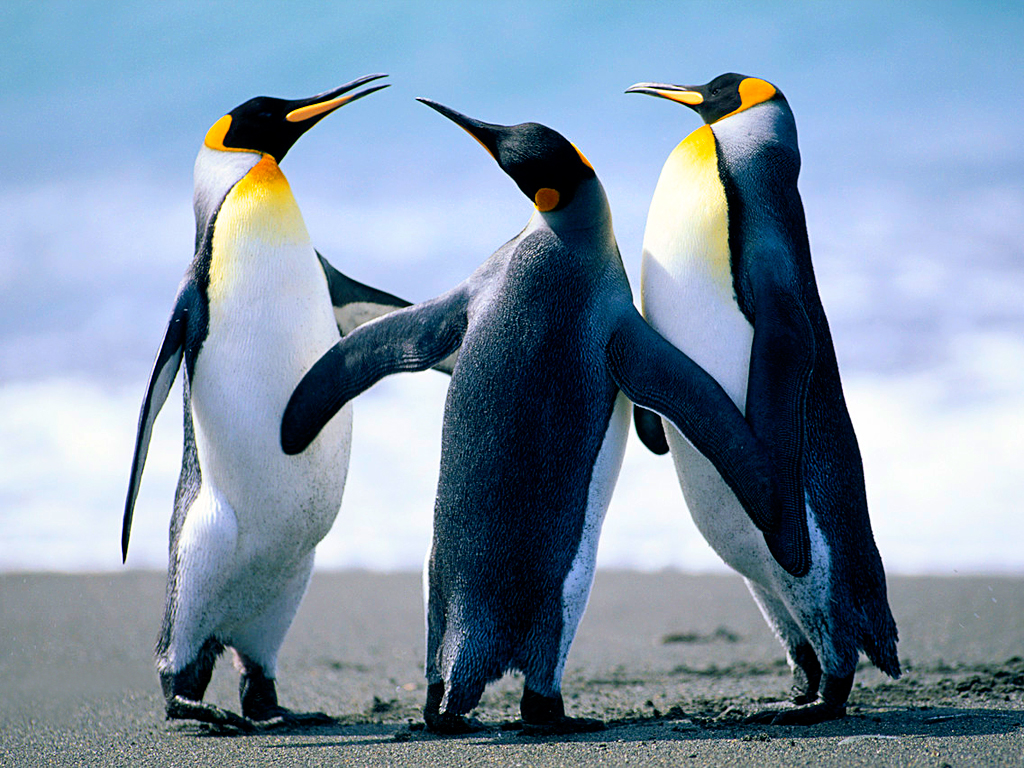
\includegraphics[scale=.50]{figures/Penguins.jpg}
\caption{TAMU figure}
\label{fig:tamu-fig5}
\end{figure}

%%%%%%%%%%%%%%%%%%%%%%%%%%%%%%%%%%%%%%%%%%%%%%%%%%%
%
%  New template code for TAMU Theses and Dissertations starting Fall 2016.
%
%
%  Author: Sean Zachary Roberson 
%	 Version 3.16.09 
%  Last updated 9/12/2016
%
%%%%%%%%%%%%%%%%%%%%%%%%%%%%%%%%%%%%%%%%%%%%%%%%%%%

%%%%%%%%%%%%%%%%%%%%%%%%%%%%%%%%%%%%%%%%%%%%%%%%%%%%%%%%%%%%%%%%%%%%%%
%%                           APPENDIX B
%%%%%%%%%%%%%%%%%%%%%%%%%%%%%%%%%%%%%%%%%%%%%%%%%%%%%%%%%%%%%%%%%%%%%

\chapter{\uppercase {A Second Appendix Whose Title Is Much Longer Than The First}}

Text for the Appendix follows.

\begin{figure}[H]
\centering
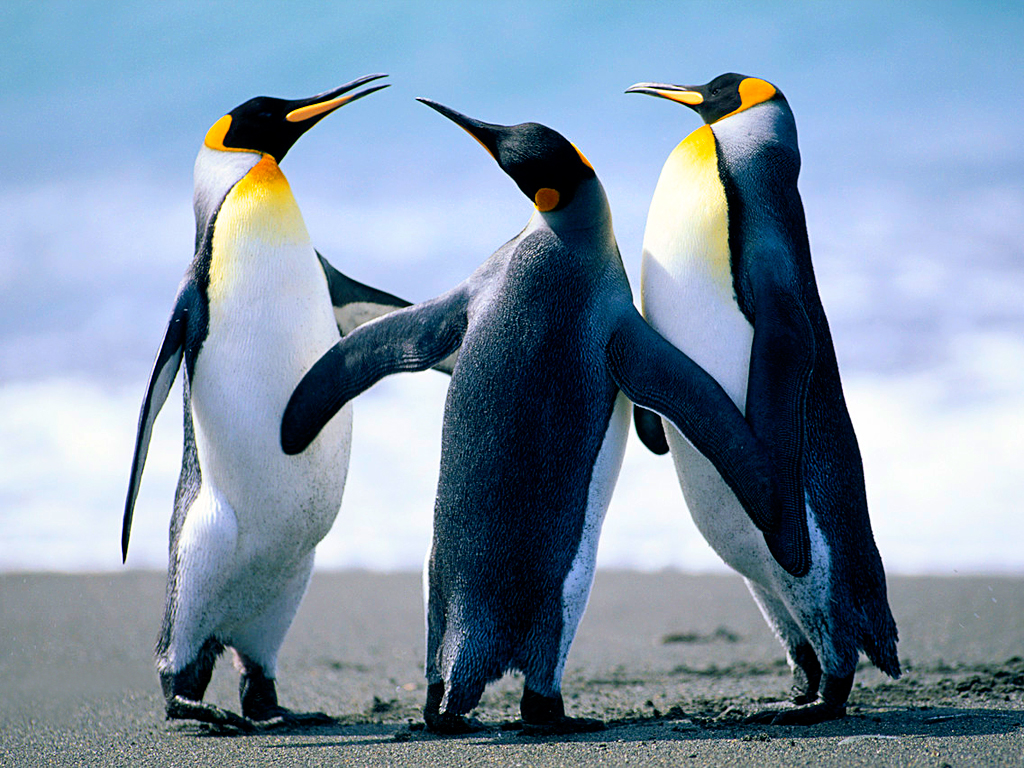
\includegraphics[scale=.50]{figures/Penguins.jpg}
\caption{Another TAMU figure.}
\label{fig:tamu-fig6}
\end{figure}

\section{Appendix Section}

\section{Second Appendix Section}


\pagebreak{}

\end{appendices}

%%%%%%%%%%%%%%%%%%%%%%%%%%%%%%%%%%%%%%%%%%%%%%%%%%%%%%%%%%%%%
\let\oldbibitem\bibitem
\renewcommand{\bibitem}{\setlength{\itemsep}{0pt}\oldbibitem}
%%%%%%%%%%%%%%%%%%%%%%%%%%%%%%%%%%%%%%%%%%%%%%%%%%%%%%%%%%%%%%%
%%%%%%%%%%%%%%%%%%%%%%%%%%%%%%%%%%%%%%%%%%%%%%%%%%%
%
%  New template code for TAMU Theses and Dissertations starting Fall 2012.  
%  For more info about this template or the 
%  TAMU LaTeX User's Group, see http://www.howdy.me/.
%
%  Author: Wendy Lynn Turner 
%	 Version 1.0 
%  Last updated 8/5/2012
%
%%%%%%%%%%%%%%%%%%%%%%%%%%%%%%%%%%%%%%%%%%%%%%%%%%%


%%%%%%%%%%%%%%%%%%%%%%%%%%%%%%%%%%%%%%%%%%%%%%%%%%%%%%%%%%%%%%%%%%%%%%
%%                           REFERENCES 
%%%%%%%%%%%%%%%%%%%%%%%%%%%%%%%%%%%%%%%%%%%%%%%%%%%%%%%%%%%%%%%%%%%%%

\phantomsection
\addcontentsline{toc}{chapter}{REFERENCES}

\renewcommand{\bibname}{{\normalsize\rm REFERENCES}}

\bibliographystyle{plain}
\bibliography{references}
%%%%%%%%%%%%%%%%%%%%%%%%%%%%%%%%%%%%%%%%%%%%%%%%%%%
%
%  New template code for TAMU Theses and Dissertations starting Fall 2012.  
%  For more info about this template or the 
%  TAMU LaTeX User's Group, see http://www.howdy.me/.
%
%  Author: Wendy Lynn Turner 
%	 Version 1.0 
%  Last updated 8/5/2012
%
%%%%%%%%%%%%%%%%%%%%%%%%%%%%%%%%%%%%%%%%%%%%%%%%%%%

\begin{appendices}
\titleformat{\chapter}{\centering\normalsize}{APPENDIX \thechapter}{0em}{\vskip .5\baselineskip\centering}
\renewcommand{\appendixname}{APPENDIX}

%%%%%%%%%%%%%%%%%%%%%%%%%%%%%%%%%%%%%%%%%%%%%%%%%%%
%
%  New template code for TAMU Theses and Dissertations starting Fall 2016.
%
%
%  Author: Sean Zachary Roberson 
%	 Version 3.16.09
%  Last updated 9/12/2016
%
%%%%%%%%%%%%%%%%%%%%%%%%%%%%%%%%%%%%%%%%%%%%%%%%%%%

%%%%%%%%%%%%%%%%%%%%%%%%%%%%%%%%%%%%%%%%%%%%%%%%%%%%%%%%%%%%%%%%%%%%%%
%%                           APPENDIX A 
%%%%%%%%%%%%%%%%%%%%%%%%%%%%%%%%%%%%%%%%%%%%%%%%%%%%%%%%%%%%%%%%%%%%%

\phantomsection

\chapter{\uppercase{First Appendix}}

Text for the Appendix follows.

\begin{figure}[H]
\centering
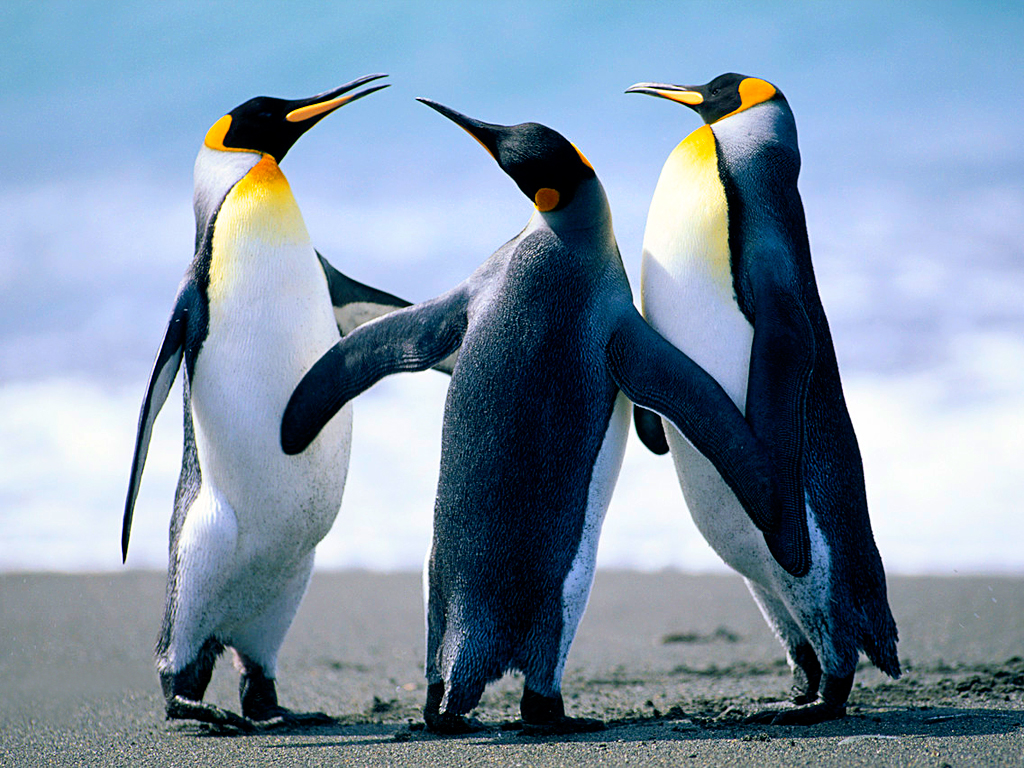
\includegraphics[scale=.50]{figures/Penguins.jpg}
\caption{TAMU figure}
\label{fig:tamu-fig5}
\end{figure}

%%%%%%%%%%%%%%%%%%%%%%%%%%%%%%%%%%%%%%%%%%%%%%%%%%%
%
%  New template code for TAMU Theses and Dissertations starting Fall 2016.
%
%
%  Author: Sean Zachary Roberson 
%	 Version 3.16.09 
%  Last updated 9/12/2016
%
%%%%%%%%%%%%%%%%%%%%%%%%%%%%%%%%%%%%%%%%%%%%%%%%%%%

%%%%%%%%%%%%%%%%%%%%%%%%%%%%%%%%%%%%%%%%%%%%%%%%%%%%%%%%%%%%%%%%%%%%%%
%%                           APPENDIX B
%%%%%%%%%%%%%%%%%%%%%%%%%%%%%%%%%%%%%%%%%%%%%%%%%%%%%%%%%%%%%%%%%%%%%

\chapter{\uppercase {A Second Appendix Whose Title Is Much Longer Than The First}}

Text for the Appendix follows.

\begin{figure}[H]
\centering
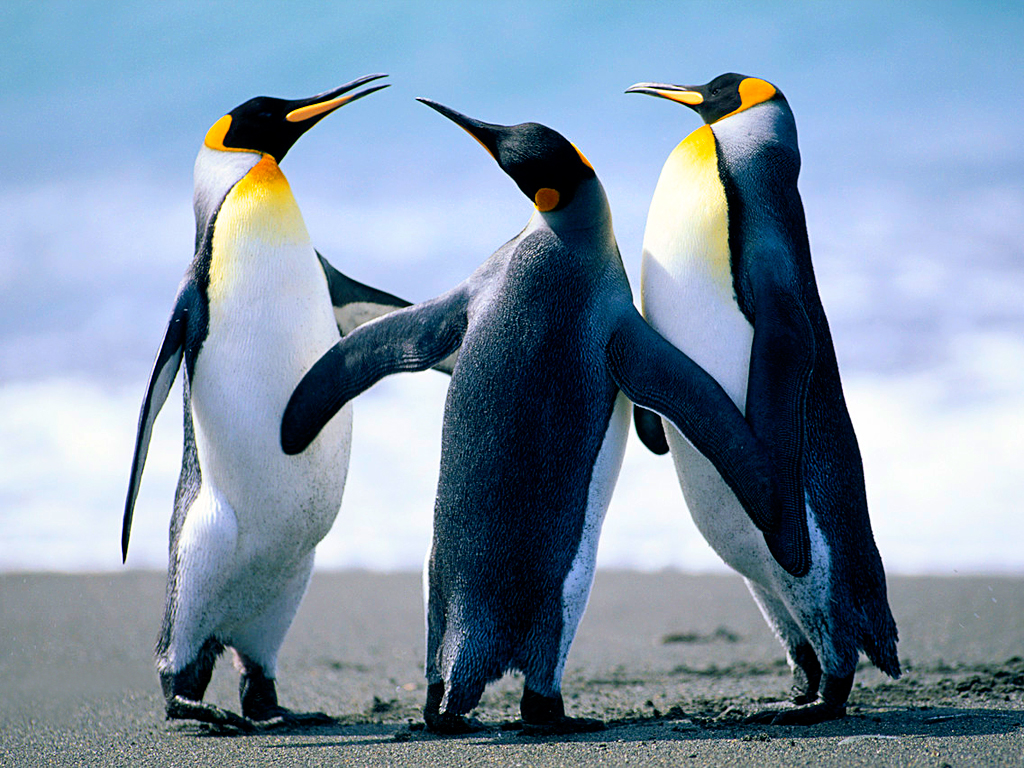
\includegraphics[scale=.50]{figures/Penguins.jpg}
\caption{Another TAMU figure.}
\label{fig:tamu-fig6}
\end{figure}

\section{Appendix Section}

\section{Second Appendix Section}


\pagebreak{}

\end{appendices}


\end{document}
